\part{Programming Techniques}\label{programming-techniques.part}


\chapter{Model Building as Software Development}

\noindent
Developing a Stan model is a software development process.  Developing
software is hard.  Very hard.  So many things can go wrong because
there are so many moving parts and combinations of parts.  

Software development practices are designed to mitigate the problems
caused by the inherent complexity of software development.
Unfortunately, many methodologies veer off into dogma, bean counting,
or both.  A couple we can recommend that provide solid, practical
advice for developers are \citep{HuntThomas:99} and
\citep{McConnell:2004}.  This section tries to summarize some of their
advice.

\section{Use Version Control}

Version control software, such as Subversion or Git, should be in
place before starting to code.%
%
\footnote{Stan started using Subversion (SVN), then switched to the
  much more feature-rich Git package.  Git does everything SVN does
  and a whole lot more.  The price is a steeper learning curve.  For
  individual or very-small-team development, SVN is just fine.}
%
It may seem like a big investment to learn version control, but it's
well worth it to be able to type a single command to revert to a
previously working version or to get the difference between the
current version and an old version.  It's even better when you need
to share work with others, even on a paper.


\section{Make it Reproducible}

Rather than entering commands on the command-line when running models
(or entering commands directly into an interactive programming
language like R or Python), try writing scripts to run the data
through the models and produce whatever posterior analysis you need.
Scripts can be written for the shell, R, or Python.  Whatever language
a script is in, it should be self contained and not depend on global
variables having been set, other data being read in, etc.  

See \refchapter{reproducibility} for complete information on
reproducibility in Stan and its interfaces.

\subsection{Scripts are Good Documentation}

It may seem like overkill if running the project is only a single line
of code, but the script provides not only a way to run the code, but
also a form of concrete documentation for what is run. 


\subsection{Randomization and Saving Seeds}

Randomness defeats reproducibility.  MCMC methods are conceptually
randomized.  Stan's samplers involve random initializations as well as
randomization during each iteration (e.g., Hamiltonian Monte Carlo
generates a random momentum in each iteration).

Computers are deterministic.  There is no real randomness, just
pseudo-random number generators.  These operate by generating a
sequence of random numbers based on a ``seed.''  Stan (and other
languages like R) can use time-based methods to generate a seed based
on the time and date, or seeds can be provided to Stan (or R) in the
form of long integers.  Stan writes out the seed used to generate the
data as well as the version number of the Stan software so that
results can be reproduced at a later date.%
%
\footnote{This also requires fixing compilers and hardware, because
  floating-point arithmetic does not have an absolutely fixed behavior
  across platforms or compilers, just operating parameters.}



\section{Make it Readable}

Treating programs and scripts like other forms of writing for an
audience provides an important perspective on how the code will be
used.  Not only might others want to read a program or model, the
developer will want to read it later.  One of the motivations of
Stan's design was to make models self-documenting in terms of variable
usage (e.g., data versus parameter), types (e.g., covariance matrix
vs. unconstrained matrix) and sizes.  

A large part of readability is consistency.  Particularly in naming
and layout.  Not only of programs themselves, but the directories and
files in which they're stored.

Readability of code is not just about comments (see
Section~\refsection{comments-programming} for commenting
recommendations and syntax in Stan).

It is surprising how often the solution to a debugging or design
problem occurs when trying to explain enough about the problem to
someone else to get help.  This can be on a mailing list, but it works
best person-to-person.  Finding the solution to your own problem when
explaining it to someone else happens so frequently in software
development that the listener is called a ``rubber ducky,'' because
they only have to nod along.%
%
\footnote{Research has shown an actual rubber ducky won't work.  For
  some reason, the rubber ducky must actually be capable of
  understanding the explanation.}


\section{Explore the Data}

Although this should go without saying, don't just fit data blindly.
Look at the data you actually have to understand its properties.  If
you're doing a logistic regression, is it separable?  If you're
building a multilevel model, do the basic outcomes vary by level?  If
you're fitting a linear regression, see whether such a model makes
sense by scatterplotting $x$ vs. $y$.

\section{Design Top-Down, Code Bottom-Up}

Software projects are almost always designed top-down from one or more
intended use cases.  Good software coding, on the other hand, is
typically done bottom-up.  

The motivation for top-down design is obvious.  The motivation for
bottom-up development is that it is much easier to develop software
using components that have been thoroughly tested.  Although Stan has
no built-in support for either modularity or testing, many of the same
principles apply.  

The way the developers of Stan themselves build models is to start as
simply as possibly, then build up. This is true even if we have a
complicated model in mind as the end goal, and even if we have a very
good idea of the model we eventually want to fit.  Rather than
building a hierarchical model with multiple interactions, covariance
priors, or other complicated structure, start simple.  Build just a
simple regression with fixed (and fairly tight) priors.  Then add
interactions or additional levels.  One at a time.  Make sure that
these do the right thing.  Then expand.

\section{Fit Simulated Data}

One of the best ways to make sure your model is doing the right thing
computationally is to generate simulated (i.e., ``fake'') data with
known parameter values, then see if the model can recover these
parameters from the data.  If not, there is very little hope that it
will do the right thing with data from the wild.  

There are fancier ways to do this, where you can do things like run
$\chi^2$ tests on marginal statistics or follow the paradigm
introduced in \citep{CookGelmanRubin:2006}, which involves interval
tests.  

\section{Debug by Print}

Although Stan does not have a stepwise debugger or any unit testing
framework in place, it does support the time-honored tradition of
debug-by-printf.
%
\footnote{The ``f'' is not a typo --- it's a historical artifact of
  the name of the \code{printf} function used for formatted printing
  in C.} 

Stan supports print statements with one or more string or expression
arguments.  Because Stan is an imperative language, variables can have
different values at different points in the execution of a program.
Print statements can be invaluable for debugging, especially for a
language like Stan with no stepwise debugger.

For instance, to print the value of variables \code{y} and
\code{z}, use the following statement.
%
\begin{quote}
\begin{Verbatim}[fontsize=\small]
print("y=", y, " z=", z);
\end{Verbatim}
\end{quote}
%
This print statement prints the string ``y='' followed by the value of
\code{y}, followed by the string `` z=''
(with the leading space), followed by the value of the variable
\code{z}.

Each print statement is followed by a new line.  The specific ASCII
character(s) generated to create a new line are platform specific.

Arbitrary expressions can be used.  For example, the statement
\begin{quote}
\begin{Verbatim}[fontsize=\small]
print("1+1=", 1+1);
\end{Verbatim}
\end{quote}
%
will print ``1 + 1 = 2'' followed by a new line.

Print statements may be used anywhere other statements may be used,
but their behavior in terms of frequency depends on how often the
block they are in is evaluated.  See \refsection{print-statements} for
more information on the syntax and evaluation of print statements.



\section{Comments}\label{comments-programming.section}

\subsection{Code Never Lies}

The machine does what the code says, not what the documentation says.
Documentation, on the other hand, might not match the code.  Code
documentation easily rots as the code evolves if the documentation is
not well maintained.  

Thus it is always preferable to write readable code as opposed to
documenting unreadable code.  Every time you write a piece of
documentation, ask yourself if there's a way to write the code in such
a way as to make the documentation unnecessary.


\subsection{Comment Styles in Stan}

Stan supports \Cpp-style comments; see \refsection{comments} for full
details.  The recommended style is to use line-based comments for
short comments on the code or to comment out one or more
lines of code.  Bracketed comments are then reserved for long
documentation comments.  The reason for this convention is that
bracketed comments cannot be wrapped inside of bracketed comments.

\subsection{What Not to Comment}

When commenting code, it is usually safe to assume that you are 
writing the comments for other programmers who understand the basics 
of the programming language in use.  In other words, don't comment the
obvious.  For instance, there is no need to have comments
such as the following, which add nothing to the code.
%
\begin{quote}
\begin{Verbatim}[fontsize=\small]
y ~ normal(0,1);  // y has a unit normal distribution
\end{Verbatim}
\end{quote}
%
A Jacobian adjustment for a hand-coded transform might be worth
commenting, as in the following example.
%
\begin{quote}
\begin{Verbatim}[fontsize=\small]
exp(y) ~ normal(0,1);
// adjust for change of vars: y = log | d/dy exp(y) |
increment_log_prob(y);
\end{Verbatim}
\end{quote}
%
It's an art form to empathize with a future code reader and decide
what they will or won't know (or remember) about statistics and Stan.

\subsection{What to Comment}

It can help to document variable declarations if variables are given
generic names like \code{N}, \code{mu}, and \code{sigma}.  For
example, some data variable declarations in an item-response model
might be usefully commented as follows.
%
\begin{quote}
\begin{Verbatim}[fontsize=\small]
int<lower=1> N;   // number of observations
int<lower=1> I;   // number of students
int<lower=1> J;   // number of test questions
\end{Verbatim}
\end{quote}
%
The alternative is to use longer names that do not require comments.
%
\begin{quote}
\begin{Verbatim}[fontsize=\small]
int<lower=1> n_obs;
int<lower=1> n_students;
int<lower=1> n_questions;
\end{Verbatim}
\end{quote}
%
Both styles are reasonable and which one to adopt is mostly a matter of
taste (mostly because sometimes models come with their own naming
conventions which should be followed so as not to confuse readers of
the code familiar with the statistical conventions).

Some code authors like big blocks of comments at the top explaining
the purpose of the model, who wrote it, copyright and licensing
information, and so on.  The following bracketed comment is an
example of a conventional style for large comment blocks.
%
\begin{quote}
\begin{Verbatim}[fontsize=\small]
/*
 * Item-Response Theory PL3 Model
 * -----------------------------------------------------
 * Copyright: Joe Schmoe  <joe@schmoe.com>
 * Date:  19 September 2012
 * License: GPLv3
 */

data {
  ...
\end{Verbatim}
\end{quote}
%
The use of leading asterisks helps readers understand the scope of the
comment.  The problem with including dates or other volatile
information in comments is that they can easily get out of synch with
the reality of the code.  A misleading comment or one that is wrong is
worse than no comment at all!


\chapter{Data Types}

\noindent
This chapter discusses the data types available for variable
declarations and expression values in Stan.  Variable types are
important for declaring parameters, checking data consistency, calling
functions, and assigning values to variables.

In Stan, every expression and variable declaration has an associated
type that is determined statically (i.e., when the program is
compiled).  Sizes of vectors, matrices, and arrays, on the other hand,
are determined dynamically (i.e., when the program is run).  This is
very different than a language like R, which lets you assign a string
to a variable and then later assign a matrix to it.

Expressions may be primitive, such as variables or constants, or they
may be composed of other components, such as a function or operator
applied to arguments.  

This chapter concentrates on the basic data types and how they are
declared, assigned, and used.  The following chapter provides a
detailed comparison of the differences among the container types:
arrays, vectors, and matrices.

\section{Basic Data Types}

Arguments for built-in and user-defined functions and local variables
are required to be basic data types, meaning an unconstrained
primitive, vector, or matrix type or an array of such.

\subsection{Primitive Types}

Stan provides two primitive data types, \code{real} for continuous
values and \code{int} for integer values.

\subsection{Vector and Matrix Types}
Stan provides three matrix-based data types, \code{vector} for column
vectors, \code{row\_vector} for row vectors, and \code{matrix} for
matrices.

\subsection{Array Types}

Any type (including the constrained types discussed in the next
section) can be made into an array type by declaring array arguments.
For example,
%
\begin{quote}
\begin{Verbatim}
real x[10];
matrix[3,3] m[6,7];
\end{Verbatim}
\end{quote}
%
declares \code{x} to be a one-dimensional array of size 10 containing
real values, and declares \code{m} to be a two-dimensional array of
size $6 \times 7$ containing values that are $3 \times 3$ matrices.


\section{Constrained Data Types}

Declarations of variables other than local variables may be provided
with constraints.  Each constrained data type corresponds to a basic
data type with constraints.

Constraints provide error checking for variables defined in the \code{data},
\code{transformed data}, \code{transformed parameters}, and 
\code{generated quantities} blocks.

Constraints are critical for variables declared in the
\code{parameters} block, where they determine the transformation from
constrained variables (those satisfying the declared constraint) to
unconstrained variables (those ranging over all of $\mathbb{R}^n$).

It is worth calling out the most important aspect of constrained data
types: 
%
\begin{quote}
\it
The model must have support (non-zero density) at every value of the
parameters that meets their declared constraints.
\end{quote}
%
If the declared parameter constraints are less strict than the
support, the samplers and optimizers may be have any of a number of
pathologies including just getting stuck, failure to initialize,
excessive Metropolis rejection, or biased samples due to inability to
explore the tails of the distribution.

\subsection{Upper and Lower Bounds}

Variables may be declared with constraints
All of the basic data types may be given lower and upper bounds using
syntax such as
%
\begin{quote}
\begin{Verbatim}
int<lower=1> N;
real<upper=0> log_p;
vector<lower=-1,upper=1>[3,3] corr;
\end{Verbatim}
\end{quote}

\subsection{Structured Vectors}

There are also special data types for structured vectors.  These are
\code{ordered} for a vector of values ordered in increasing order, and
\code{positive\_ordered} for a vector of positive values ordered in
increasing order.  

There is also a type \code{simplex} for vectors of non-negative values
that sum to one, and \code{unit\_vector} for vectors of values whose
squares sum to one.

\subsection{Structured Matrices}

Symmetric, positive-definite matrices have the type
\code{cov\_matrix}.  Correlation matrices, which are symmetric
positive-definite matrices with unit diagonals, have the type
\code{corr\_matrix}.

There is also a pair of Cholesky factor types.  The first,
\code{cholesky\_factor\_cov}, is for Cholesky factors of symmetric,
positive definite matrices, which amounts to being a lower-triangular
matrix with positive diagonal elements.  The second, and
\code{cholesky\_factor\_corr}, is for Cholesky factors of correlation
matrices, which amounts to being a lower-triangular matrix with
positive diagonal elements, where additionally the length of each row
is 1.  Using Cholesky factor types can be much more efficient than the
full correlation or covariance matrices because they are easier to
factor and scale.



\section{Assignment and Argument Passing}

\subsection{Assignment}

Constrained data values may be assigned to unconstrained variables of
matching basic type and vice-versa.   Matching is interpreted strictly
as having the same basic type and number of array dimensions.
Constraints are not considered, but basic data types are.  

Arrays cannot be assigned to vectors and vice-versa.  Similarly,
vectors cannot be assigned to matrices and vice-versa, even if their
dimensions conform.  \refchapter{containers} provides more information
on the distinctions between vectors and arrays and when each is
appropriate.

\subsection{Function Invocation}

Passing arguments to functions in Stan works just like assignment to
basic types.  Stan functions are only specified for the basic data
types of their arguments, including array dimensionality, but not for
sizes or constraints.  Of course, functions often check constraints as
part of their behavior.  



\chapter{Containers: Arrays, Vectors, and Matrices}\label{containers.chapter}

\noindent
Stan provides three types of container objects: arrays, vectors, and
matrices.  The three types are not interchangeable.  Vectors, matrices,
and arrays are not assignable to one another, even if their dimensions
are identical.  A $3 \times 4$ matrix is a different kind of object in
Stan than a $3 \times 4$ array. 

\section{Vectors and Matrices}

Vectors and matrices are more limited kinds of data structures than
arrays.  Vectors are intrinsically one-dimensional collections of
reals, whereas matrices are intrinsically two dimensional. 

The intention of using matrix types is to call out their usage in the
code.  There are three situations in Stan where {\it only} vectors and
matrices may be used,
%
\begin{itemize}
\item matrix arithmetic operations (e.g., matrix multiplication)
\item linear algebra functions (e.g., eigenvalues and determinants),
  and
\item multivariate function parameters and outcomes (e.g.,
  multivariate normal distribution arguments).
\end{itemize}
%

Vectors and matrices cannot be typed to return integer values.  They
are restricted to \code{real} values.%
%
\footnote{This may change if Stan is called upon to do complicated
  integer matrix operations or boolean matrix operations.  Integers
  are not appropriate inputs for linear algebra functions.}

\section{Arrays}

Arrays, on the other hand, are intrinsically one-dimensional
collections of other kinds of objects.  The values in an array can be
any type, so that arrays may contain values that are simple reals or
integers, vectors, matrices, or other arrays.  Arrays are the only way
to store sequences of integers, and some functions in Stan, such as
discrete distributions, require integer arguments. 


A two-dimensional array is just an array of arrays, both conceptually
and in terms of current implementation.  When an index is supplied to
an array, it returns the value at that index.  When more than one
index is supplied, this idexing operation is chained.  For example, if
\code{a} is a two-dimensional array, then \code{a[m,n]} is just
a convenient shorthand for \code{a[m][n]}.


\section{Efficiency Considerations}

One of the motivations for Stan's underlying design is efficiency.

The underlying matrix and linear algebra operations are implemented in
terms of data types from the Eigen \Cpp library.  By having vectors
and matrices as basic types, no conversion is necessary when invoking
matrix operations or calling linear algebra functions.  

Arrays, on the other hand, are implemented as instances of the \Cpp \ 
\code{std::vector} class (not to be confused with Eigen's
\code{Eigen::Vector} class or Stan vectors).  By implementing arrays
this way, indexing is very efficient because values can be returned by
reference rather than copied by value.

\subsection{Matrices vs.\ Two-Dimensional Arrays}

In Stan models, there are a few minor efficiency considerations in
deciding between a two-dimensional array and a matrix, which may seem
interchangeable at first glance.  

First, matrices use a bit less memory than two-dimensional arrays.
This is because they don't store a sequence of arrays, but just the
data and the two dimensions.  

Second, matrices store their data in column-major order.  Furthermore,
all of the data in a matrix is guaranteed to be contiguous in memory.
This is an important consideration for optimized code because bringing
in data from memory to cache is much more expensive than performing
arithmetic operations with contemporary CPUs.  Arrays, on the other
hand, only guarantee that the values of primitive types are contiguous
in memory; otherwise, they hold copies of their values (which are
returned by reference wherever possible).

Third, both data structures are best traversed in the order in which
they are stored.  This also helps with memory locality.  This is
column-major for matrices, so the following order is appropriate.
%
\begin{quote}
\begin{Verbatim}
matrix[M,N] a;
...
for (n in 1:N)
  for (m in 1:M)
    ... do something with a[m,n] ...
\end{Verbatim}
\end{quote}
%
Arrays, on the other hand, should be traversed in row-major (or
first-index fastest) order.%
%
\begin{quote}
\begin{Verbatim}
real a[M,N];
...
for (m in 1:M)
  for (n in 1:N)
    ... do something with a[m,n] ...
\end{Verbatim}
\end{quote}
%
The first use of \code{a[m,n]} should bring \code{a[m]} into memory.
Overall, traversing matrices is more efficient than traversing arrays.

This is true even for arrays of matrices.  For example, the ideal
order in which to traverse a two-dimensional array of matrices is
%
\begin{quote}
\begin{Verbatim}
matrix[M,N] b[I,J];
...
for (i in 1:I)
  for (j in 1:J)
    for (n in 1:N)
      for (m in 1:M)
        ... do something with b[i,j,m,n] ...
\end{Verbatim}
\end{quote}

If \code{a} is a matrix, the notation \code{a[m]} picks out row
\code{m} of that matrix.  This is a rather inefficient operation for
matrices.  If indexing of vectors is needed, it is much better to
declare an array of vectors.  That is, this
%
\begin{quote}
\begin{Verbatim}
row_vector[N] b[M];
...
for (m in 1:M)
   ... do something with row vector b[m] ...
\end{Verbatim}
\end{quote}
%
is much more efficient than the pure matrix version
%
\begin{quote}
\begin{Verbatim}
matrix b[M,N];
...
for (m in 1:M)
   ... do something with row vector b[m] ...
\end{Verbatim}
\end{quote}
%
Similarly, indexing an array of column vectors is more efficient than
using the \code{col} function to pick out a column of a matrix.

In contrast, whatever can be done as pure matrix algebra will be the
fastest.  So if I want to create a row of predictor-coefficient
dot-products, it's more efficient to do this
%
\begin{quote}
\begin{Verbatim}
matrix[N,K] x;    // predictors (aka covariates)
...
vector[K] beta;   // coeffs
...
vector[N] y_hat;  // linear prediction
...
y_hat <- x * beta;
\end{Verbatim}
\end{quote}
%
than it is to do this
%
\begin{quote}
\begin{Verbatim}
row_vector[K] x[N];    // predictors (aka covariates)
...
vector[K] beta;   // coeffs
...
vector[N] y_hat;  // linear prediction
...
for (n in 1:N)
  y_hat[n] <- x[n] * beta;
\end{Verbatim}
\end{quote}

\subsection{(Row) Vectors vs. One-Dimensional Arrays}

For use purely as a container, there is really nothing to decide among
vectors, row vectors and one-dimensional arrays.  The
\code{Eigen::Vector} template specialization and the
\code{std::vector} template class are implemented very similarly as
containers of \code{double} values (the type \code{real} in Stan).
Only arrays in Stan are allowed to store integer values.



\chapter{Regression Models}

\noindent
\Stan supports regression models from simple linear regressions to
multilevel generalized linear models.  

\section{Linear Regression}

The simplest linear regression model is the following, with a single
predictor and a slope and intercept coefficient, and normally
distributed noise.  This model can be written using standard
regression notation as
%
\[
y_n = \alpha + \beta x_n + \epsilon_n
\ \ \ \mbox{where} \ \ \ 
\epsilon_n \sim \distro{Normal}(0,\sigma).
\]
This is equivalent to the following sampling involving the
residual,
\[
y_n - (\alpha + \beta X_n) \sim \distro{Normal}(0,\sigma),
\]
and reducing still further, to
\[
y_n \sim \distro{Normal}(\alpha + \beta X_n, \, \sigma).
\]
%
This latter form of the model is coded in \Stan as follows.
%
\begin{quote}
\begin{Verbatim}[fontsize=\small]
data {
  int<lower=0> N;
  vector[N] x;
  vector[N] y;
}
parameters {
  real alpha;
  real beta;
  real<lower=0> sigma;
}
model {
  for (n in 1:N)
    y[n] ~ normal(alpha + beta * x[n], sigma);
}
\end{Verbatim}
\end{quote}
%
There are \code{N} observations, each with predictor \code{x[n]} and
outcome \code{y[n]}.  The intercept and slope parameters are
\code{alpha} and \code{beta}.  The model assumes a normally
distributed noise term with scale \code{sigma}.  This model has
improper priors for the two regression coefficients.

\subsection{Matrix Notation and Vectorization}

The sampling statement in the previous model can be vectorized and
written equivalently as follows:
%
\begin{quote}
\begin{Verbatim}
model {
  y ~ normal(alpha + beta * x, sigma);
}
\end{Verbatim}
\end{quote}
%
The main difference is that the vectorized form is much faster.%
%
\footnote{Unlike in Python and R, which are interpreted, Stan is
  translated to \Cpp and compiled, so loops and assignment statements
  are fast.  Vectorized code is faster in Stan because (a) the
  expression tree used to compute derivatives can be simplified,
  leading to fewer virtual function calls, and (b) computations that
  would be repeated in the looping version, such as \code{log(sigma)}
  in the above model, will be computed once and reused.}

In general, Stan allows the arguments to distributions such as
\code{normal} to be vectors.  If any of the other arguments are
vectors or arrays, they have to be the same size.  If any of the other
arguments is a scalar, it is reused for each vector entry.  See
\refchapter{vectorization} for more information on vectorization.

The other reason this works is that Stan's arithmetic operators are
overloaded to perform matrix arithmetic on matrices.  In this case,
because \code{x} is of type \code{vector} and \code{beta} of type
\code{real}, the expression \code{beta * x} is of type \code{vector}.
Because Stan supports vectorization, a regression model with more than
one predictor can be written directly using matrix notation.
%
\begin{quote}
\begin{Verbatim}
data {
  int<lower=0> N;   // number of data items
  int<lower=0> K;   // number of predictors
  matrix[N,K] x;    // predictor matrix
  vector[N] y;      // outcome vector
}
parameters {
  real alpha;           // intercept
  vector[K] beta;       // coefficients for predictors
  real<lower=0> sigma;  // error scale
}
model {
  y ~ normal(x * beta, sigma);  // likelihood
}
\end{Verbatim}
\end{quote}
%
The constraint \code{lower=0} in the declaration of \code{sigma}
constrains the value to be greater than or equal to 0.  With no prior
in the model block, the effect is an improper prior on non-negative
real numbers.  Althogh a more informative prior may be added, improper
priors are acceptable as long as they lead to proper posteriors.

In the model above, \code{x} is an $N \times K$ matrix of predictors
and \code{beta} a $K$-vector of coefficients, so \code{x * beta} is an
$N$-vector of predictions, one for each of the $N$ data items.  These
predictions line up with the outcomes in the $N$-vector \code{y}, so
the entire model may be written using matrix arithmetic as shown.

The sampling statement in the model above is just a more efficient,
vector-based approach to coding the model with a loop, as in the
following statistically equivalent model.
%
\begin{quote}
\begin{Verbatim}
model {
  for (n in 1:N)
    y[n] ~ normal(x[n] * beta, sigma);
}
\end{Verbatim}
\end{quote}
%
With Stan's matrix indexing scheme, \code{x[n]} picks out row \code{n}
of the matrix \code{x};  because \code{beta} is a column vector, 
the product \code{x[n] * beta} is a scalar of type \code{real}.

\subsubsection{Intercepts as Inputs}

In the model formulation
%
\begin{quote}
\begin{Verbatim}
  y ~ normal(x * beta, sigma);
\end{Verbatim}
\end{quote}
%
there is no longer an intercept coefficient \code{alpha}.  Instead, we
have assumed that the first column of the input matrix \code{x} is a
column of 1 values.  This way, \code{beta[1]} plays the role of the
intercept.  If the intercept gets a different prior than the the slope
terms, then it would be clearer to break it out.  It is also slightly
more efficient in its explicit form with the intercept variable
singled out because there's one fewer multiplications; it should not
make that much of a difference to speed, though, so the choice should
be based on clarity.


\section{Priors for Coefficients and Scales}\label{regression-priors.section}

This section describes the choices available for modeling priors for
regression coefficients and scales.  Priors for univariate parameters
in hierarchical models are discussed in
\refsection{hierarchical-priors} and multivariate parameters in
\refsection{multivariate-hierarchical-priors}. There is also a
discussion of priors used to identify models in
\refsection{priors-for-identification}.

\subsection{Background Reading}

See \citep{Gelman:2006} for more an overview of choices for priors for
scale parameters, \citep{ChungEtAl:2013} for an overview of choices
for scale priors in penalized maximum likelihood estimates, and
\cite{GelmanJakulinPittauEtAl:2008} for a discussion of prior choice
for regression coefficients.

\subsection{Improper Uniform Priors}

The default in Stan is to provide uniform (or ``flat'') priors on
parameters over their legal values as determined by their declared
constraints.  A parameter declared without constraints is thus given a
uniform prior on $(-\infty,\infty)$ by default, whereas a scale
parameter declared with a lower bound of zero gets an improper uniform
prior on $(0,\infty)$.  Both of these priors are improper in the sense
that there is no way formulate a density function for them that
integrates to 1 over its support.

Stan allows models to be formulated with improper priors, but in order
for sampling or optimization to work, the data provided must ensure a
proper posterior.  This usually requires a minimum quantity of data,
but can be useful as a starting point for inference and as a baseline
for sensitivity analysis (i.e., considering the effect the prior
has on the posterior).

\subsection{Uniform Priors and Transforms}

Uniform priors are specific to the scale on which they are formulated.
For instance, we could give a scale parameter $\sigma > 0$ a uniform
prior on $(0,\infty)$, $q(\sigma) = c$ (we use $q$ because the
``density'' is not only unnormalized, but unnormalizable), or we could
work on the log scale and provide $\log \sigma$ a uniform prior on
$(-\infty,\infty)$, $q(\log \sigma) = c$.  These work out to be
different priors on $\sigma$ due to the Jacobian adjustment necessary
for the log transform; see \refsection{change-of-variables} for more
information on changes of variables and their requisite Jacobian
adjustments.

Stan automatically applies the necessary Jacobian adjustment for
variables declared with constraints to ensure a uniform density on the
legal constrained values.  This Jacobian adjustment is turned off when
optimization is being applied in order to produce appropriate maximum
likelihood estimates.

\subsection{``Uninformative'' Proper Priors}

It is not uncommon to see models with priors on regression
coefficients such as $\distro{Normal}(0,1000)$.%
%
\footnote{The practice was common in BUGS and can be seen in most of
  their examples \cite{LunnEtAl:2012}.}
%
If the prior scale, such as 1000, is several orders of magnitude
larger than the estimated coefficients, then such a prior is
effectively providing no effect whatsoever.  

We actively discourage users from using the default scale priors
suggested through the BUGS examples \citep{LunnEtAl:2012}, such as
\[
\sigma^2 \sim \distro{InvGamma}(0.001, 0.001).
\]
%
Such priors concentrate too much probability mass outside of
reasonable posterior values, and unlike the symmetric wide normal
priors, can have the profound effect of skewing posteriors; see
\citep{Gelman:2006} for examples and discussion.

\subsection{Truncated Priors}

If a variable is declared with a lower bound of zero, then assigning
it a normal prior in a Stan model produces the same effect as
providing a properly truncated half-normal prior.  The truncation at
zero need not be specified as Stan only requires the density up to a
proportion.  So a variable declared with
%
\begin{quote}
\begin{Verbatim}
real<lower=0> sigma;
\end{Verbatim}
\end{quote}
%
and given a prior
\begin{quote}
\begin{Verbatim}
sigma ~ normal(0,1000);
\end{Verbatim}
\end{quote}
%
gives \code{sigma} a half-normal prior, technically
%
\[
p(\sigma) 
\ = \
\frac{\distro{Normal}(\sigma|0,1000)}
     {1 - \distro{NormalCDF}(0|0,1000)}
\ \propto \
\distro{Normal}(\sigma|0,1000),
\]
%
but Stan is able to avoid the calculation of the normal cumulative
distribution (CDF) function required to normalize the half-normal density.
If either the prior location or scale is a parameter or if the
truncation point is a parameter, the truncation cannot be dropped,
because the normal CDF term will not be a constant.


\subsection{Weakly Informative Priors}

Typically a researcher will have some knowledge of the scale of the
variables being estimated.  For instance, if we're estimating an
intercept-only model for the mean population height for adult women,
then we know the answer is going to be somewhere in the one to three
meter range.  That gives us information around which to form a weakly
informative prior.

Similarly, logistic regression with predictors on the standard scale
(roughly zero mean, unit variance), then it is unlikely to have a
coefficient that's larger than five in absolute value.  In these
cases, it makes sense to provide a weakly informative prior such as
$\distro{Normal}(0,5)$ for such a coefficient.

Weakly informative priors help control inference computationally and
statistically.  Computationally, a prior increases the curvature
around the volume where the solution is expected to lie, which in turn
guides both gradient-based like L-BFGS and Hamiltonian Monte Carlo
sampling by not allowing them to stray too far from the location of a
surface.  Statistically, a weakly informative prior is more sensible
for a problem like women's mean height, because a very diffuse prior
like $\distro{Normal}(0,1000)$ will ensure that the vast majority of
the prior probability mass is outside the range of the expected
answer, which can overwhelm the inferences available from a small data
set.

\subsection{Bounded Priors}

Consider the women's height example again.  One way to formulate a
proper prior is to impose a uniform prior on a bounded scale.  For
example, we could declare the parameter for mean women's height to
have a lower bound of one meter and an upper bound of three meters.
Surely the answer has to lie in that range.  

Similarly, it is not uncommon to see priors for scale parameters that
impose lower bounds of zero and upper bounds of very large numbers,
such as 10,000.%
%
\footnote{This was also a popular strategy in the BUGS example models
  \citep{LunnEtAl:2012}, which often went one step further and set the
  lower bounds to a small number like 0.001 to discourage numerical
  underflow to zero.}
%
This provides roughly the same problem for estimation as a very
diffuse inverse gamma prior on variance.  We prefer to leave
parameters which are not absolutely physically constrained to float
and provide them informative priors.  In the case of women's height,
such a prior might be $\distro{Normal}(2,0.5)$ on the scale of meters;
it concentrates 95\% of its mass in the interval $(1,3)$, but still
allows values outside of that region.

In cases where bounded priors are used, the posterior fits should be
checked to make sure the parameter is not estimated at or very close
to a boundary.  This will not only cause computational problems, it
indicates a problem with the way the model is formulated.  In such
cases, the interval should be widened to see where the parameter fits
without such constraints, or boundary-avoid priors should be used (see
\refsection{hierarchical-priors}.)

\subsection{Fat-Tailed Priors and ``Default'' Priors}

A reasonable alternative if we want to accomodate outliers is to use a
prior that concentrates most of mass around the area where values are
expected to be, but still leaves a lot of mass in its tails.  The
usual choice in such a situation is to use a Cauchy distribution for a
prior, which can concentrate its mass around its median, but has tails
that are so fat that the variance is infinite.  

Without specific information, the Cauchy prior is a very good default
parameter choice for regression coefficients
\citep{GelmanJakulinPittauEtAl:2008} and the half-Cauchy (coded
implicitly in Stan) a good default choice for scale parameters
\citep{Gelman:2006}.



\subsection{Informative Priors}

Ideally, there will be substantive information about a problem that
can be included in an even tighter prior than a weakly informative
prior.  This may come from actual prior experiments and thus be the
posterior of other data, it may come from meta-analysis, or it may
come simply by soliciting it from domain experts.  All the goodness of
weakly informative priors applies, only with more strength.

\subsection{Conjugacy}

Unlike in Gibbs sampling, there is no computational advantage to
providing conjugate priors (i.e., priors that produce posteriors in
the same family) in a Stan program.%
%
\footnote{BUGS and JAGS both support conjugate sampling through Gibbs
  sampling.  JAGS extended the range of conjugacy that could be
  exploited with its GLM module.  Unlike Stan, both BUGS and JAGS are
  restricted to conjugate priors for constrained multivariate
  quantities such as covariance matrices or simplexes.}
%
Neither the Hamiltonian Monte Carlo samplers or the optimizers make
use of conjugacy, working only on the log density and its derivatives.



\section{Robust Noise Models}

The standard approach to linear regression is to model the noise
term $\epsilon$ as having a normal distribution.  From \Stan's
perspective, there is nothing special about normally distributed
noise.  For instance, robust regression can be accommodated by giving
the noise term a Student-$t$ distribution.  To code this in \Stan, the
sampling distribution is changed to the following.
%
\begin{quote}
\begin{Verbatim}[fontsize=\small]
data {
  ...
  real<lower=0> nu;
}
...
model {
  for (n in 1:N)
    y[n] ~ student_t(nu, alpha + beta * x[n], sigma);
}
\end{Verbatim}
\end{quote}
%
The degrees of freedom constant \code{nu} is specified as data.

\section{Logistic and Probit Regression}\label{logistic-probit-regression.section}

For binary outcomes, either of the closely related logistic or probit
regression models may be used.  These generalized linear models vary
only in the link function they use to map linear predictions in
$(-\infty,\infty)$ to probability values in $(0,1)$.  Their respective
link functions, the logistic function and the unit normal cumulative distribution
function, are both sigmoid functions (i.e., they are both {\it S}-shaped).

A logistic regression model with one predictor and an intercept is coded as
follows.
%
\begin{quote}
\begin{Verbatim}[fontsize=\small]
data {
  int<lower=0> N;
  vector[N] x;
  int<lower=0,upper=1> y[N];
}
parameters {
  real alpha;
  real beta;
}
model {
  y ~ bernoulli_logit(alpha + beta * x);
} 
\end{Verbatim}
\end{quote}
%
The noise parameter is built into the Bernoulli formulation here
rather than specified directly.  

Logistic regression is a kind of generalized linear model with binary
outcomes and the log odds (logit) link function, defined by
%
\[
\mbox{logit}(v) = \log \left( \frac{v}{1-v} \right).
\]
%
The inverse of the link function appears in the model.  
%
\[
\mbox{logit}^{-1}(u) = \frac{1}{1 + \exp(-u)}.
\]
%

The model formulation above uses the logit-parameterized version of
the Bernoulli distribution, which is defined by 
%
\[
\distro{BernoulliLogit}(y|\alpha) 
=
\distro{Bernoulli}(y | \mbox{logit}^{-1}(\alpha)).
\]
%
The formulation is also vectorized in the sense that \code{alpha} and
\code{beta} are scalars and \code{x} is a vector, so that \code{alpha
  + beta * x} is a vector.  The vectorized formulation is equivalent
to the less efficient version
%
\begin{quote}
\begin{Verbatim}
for (n in 1:N)
  y[n] ~ bernoulli_logit(alpha + beta * x[n]);
\end{Verbatim}
\end{quote}
%
Expanding out the Bernoulli logit, the model is equivalent to the more
explicit, but less efficient and less arithmetically stable
%
\begin{quote}
\begin{Verbatim}
for (n in 1:N)
  y[n] ~ bernoulli(inv_logit(alpha + beta * x[n]));
\end{Verbatim}
\end{quote}

Other link functions may be used in the same way.  For example, probit
regression uses the cumulative normal distribution function, which is
typically written as 
\[
\Phi(x) = \int_{-\infty}^x \distro{Normal}(y|0,1) \, dy.
\]
%
The cumulative unit normal distribution function $\Phi$ is implemented
in \Stan as the function \code{Phi}.  The probit regression model
may be coded in \Stan by replacing the logistic model's sampling
statement with the following.
%
\begin{quote}
\begin{Verbatim}[fontsize=\small]
        y[n] ~ bernoulli(Phi(alpha + beta * x[n]));
\end{Verbatim}
\end{quote}
%
A fast approximation to the cumulative unit normal distribution function 
$\Phi$ is implemented in \Stan as the function \code{Phi\_approx}.  The 
approximate probit regression model may be coded with the following.
%
\begin{quote}
\begin{Verbatim}[fontsize=\small]
        y[n] ~ bernoulli(Phi_approx(alpha + beta * x[n]));
\end{Verbatim}
\end{quote}

\section{Multi-Logit Regression}

Multiple outcome forms of logistic regression can be coded directly in
\Stan.  For instance, suppose there are $K$ possible outcomes for each
output variable $y_n$.  Also suppose that there is a $D$-dimensional
vector $x_n$ of predictors for $y_n$.  The multi-logit model with
$\distro{Normal}(0,5)$ priors on the coefficients is coded as follows.
%
\begin{quote}
\begin{Verbatim}[fontsize=\small]
data {
  int K;
  int N;
  int D;
  int y[N];
  vector[D] x[N];
}
parameters {
  matrix[K,D] beta;
}
model {
  for (k in 1:K)
    for (d in 1:D)
      beta[k,d] ~ normal(0,5);
  for (n in 1:N)
    y[n] ~ categorical(softmax(beta * x[n]));
}
\end{Verbatim}
\end{quote}
%

The softmax function is defined for a $K$-vector $\gamma \in \reals^K$ by
\[
\mbox{softmax}(\gamma) = 
\left(
 \frac{\exp(\gamma_1)}
      {\sum_{k=1}^K \exp(\gamma_k)},
  \ldots,
  \frac{\exp(\gamma_K)}
       {\sum_{k=1}^K \exp(\gamma_k)}
\right).
\]
%
The result is in the unit $K$-simplex and thus appropriate to use as
the parameter for a categorical distribution.

\subsubsection{Constraints on Data Declarations}

The data block in the above model is defined without constraints on
sizes \code{K}, \code{N}, and \code{D} or on the outcome array
\code{y}.  Constraints on data declarations provide error checking at
the point data is read (or transformed data is defined), which is
before sampling begins.  Constraints on data declarations also make
the model author's intentions more explicit, which can help with
readability.  The above model's declarations could be tightened to
%
\begin{quote}
\begin{Verbatim}
  int<lower=2> K;
  int<lower=0> N;
  int<lower=1> D;
  int<lower=1,upper=K> y[N];
\end{Verbatim}
\end{quote}
%
These constraints arise because the number of categories, \code{K},
must be at least two in order for a categorical model to be useful.
The number of data items, \code{N}, can be zero, but not negative;
unlike R, Stan's for-loops always move forward, so that a loop extent
of \code{1:N} when \code{N} is equal to zero ensures the loop's body
will not be executed.  The number of predictors, \code{D}, must be at
least one in order for \code{beta * x[n]} to produce an
appropriate argument for \code{softmax()}.  The categorical outcomes
\code{y[n]} must be between \code{1} and \code{K} in order for the
discrete sampling to be well defined.

Constraints on data declarations are optional.  Constraints on
parameters declared in the \code{parameters} block, on the other hand,
are {\it not}\ optional---they are required to ensure support for all
parameter values satisfying their constraints.  Constraints on
transformed data, transformed parameters, and generated quantities are
also optional.

\subsection{Identifiability}

Because softmax is invariant under adding a constant to each component
of its input, the model is typically only identified if there is a
suitable prior on the coefficients.

An alternative is to use $K-1$ vectors by fixing one of them to be
zero.  See \refsection{partially-known-parameters} for an example of
how to mix known quantities and unknown quantities in a vector.


\section{Ordered Logistic and Probit Regression}\label{ordered-logistic.section}

Ordered regression for an outcome $y_n \in \setlist{1,\ldots,K}$ with
predictors $x_n \in \reals^D$ is determined by a single coefficient
vector $\beta \in \reals^D$ along with a sequence of cutpoints $c \in
\reals^{D-1}$ sorted so that $c_d < c_{d+1}$.  The discrete output is
$k$ if the linear predictor $x_n \beta$ falls between $c_{k-1}$ and
$c_k$, assuming $c_0 = -\infty$ and $c_K = \infty$.  The noise term is
fixed by the form of regression, with examples for ordered logistic
and ordered probit models.  

\subsection{Ordered Logistic Regression}

The ordered logistic model can be coded in \Stan using the
\code{ordered} data type for the cutpoints and the built-in
\code{ordered\_logistic} distribution.
%
\begin{quote}
\begin{Verbatim}[fontsize=\small]
data {
  int<lower=2> K;
  int<lower=0> N;
  int<lower=1> D;
  int<lower=1,upper=K> y[N];
  row_vector[D] x[N];
} 
parameters {
  vector[D] beta;
  ordered[K-1] c;
} 
model {
  for (n in 1:N)
    y[n] ~ ordered_logistic(x[n] * beta, c);
}
\end{Verbatim}
\end{quote}
% 
The vector of cutpoints \code{c} is declared as \code{ordered[K-1]},
which guarantees that \code{c[k]} is less than \code{c[k+1]}. 

If the cutpoints were assigned independent priors, the constraint
effectively truncates the joint prior to support over points that
satisfy the ordering constraint.  Luckily, \Stan does not need to
compute the effect of the constraint on the normalizing term because
the probability is needed only up to a proportion.


\subsubsection{Ordered Probit}

An ordered probit model could be coded in exactly the same way by
swapping the cumultive logistic (\code{inv\_logit}) for the cumulative
normal (\code{Phi}).
%
\begin{quote}
\begin{Verbatim}[fontsize=\small]
data {
  int<lower=2> K;
  int<lower=0> N;
  int<lower=1> D;
  int<lower=1,upper=K> y[N];
  row_vector[D] x[N];
}
parameters {
  vector[D] beta;
  ordered[K-1] c;
}
model {
  vector[K] theta;
  for (n in 1:N) {
    real eta;
    eta <- x[n] * beta;
    theta[1] <- 1 - Phi(eta - c[1]);
    for (k in 2:(K-1))
      theta[k] <- Phi(eta - c[k-1]) - Phi(eta - c[k]);
    theta[K] <- Phi(eta - c[K-1]);
    y[n] ~ categorical(theta);
  }
}
\end{Verbatim}
\end{quote}
%
The logistic model could also be coded this way by replacing
\code{Phi} with \code{inv\_logit}, though the built-in encoding based
on the softmax transform is more efficient and more numerically
stable.  A small efficiency gain could be achieved by computing the
values \code{Phi(eta - c[k])} once and storing them for re-use.


\section{Hierarchical Logistic Regression}

The simplest multilevel model is a hierarchical model in which the
data is grouped into $L$ distinct categories (or levels).  An extreme approach would be to
completely pool all the data and estimate a common vector of
regression coefficients $\beta$.  At the other extreme, an approach
would no pooling assigns each level $l$ its own coefficient vector
$\beta_l$ that is estimated separately from the other levels.  A
hierarchical model is an intermediate solution where the degree of
pooling is determined by the data and a prior on the amount of
pooling.

Suppose each binary outcome $y_n \in \setlist{0,1}$ has an associated
level, $ll_n \in \setlist{1,\ldots,L}$.  Each outcome will also have
an associated predictor vector $x_n \in \reals^D$.  Each level $l$
gets its own coefficient vector $\beta_l \in \reals^D$.  The
hierarchical structure involves drawing the coefficients $\beta_{l,d}
\in \reals$ from a prior that is also estimated with the data.  This
hierarchically estimated prior determines the amount of pooling.  If
the data in each level are very similar, strong pooling will be
reflected in low hierarchical variance.  If the data in the levels are
dissimilar, weaker pooling will be reflected in higher hierarchical variance.

The following model encodes a hierarchical logistic regression model
with a hierarchical prior on the regression coefficients.
%
\begin{quote}
\begin{Verbatim}[fontsize=\small]
data {
  int<lower=1> D;
  int<lower=0> N;
  int<lower=1> L;
  int<lower=0,upper=1> y[N];
  int<lower=1,upper=L> ll[N];
  row_vector[D] x[N];
}
parameters {
  real mu[D];
  real<lower=0,upper=1000> sigma[D];
  vector[D] beta[L];
}
model {
  for (d in 1:D) {
    mu[d] ~ normal(0,100);
    for (l in 1:L)
      beta[l,d] ~ normal(mu[d],sigma[d]);
  }
  for (n in 1:N)
    y[n] ~ bernoulli(inv_logit(x[n] * beta[ll[n]]));
}
\end{Verbatim}
\end{quote}  
%

\subsubsection{Optimizing the Model}

Where possible, vectorizing sampling statements leads to faster log
probability and derivative evaluations.  The speed boost is not
because loops are eliminated, but because vectorization allows sharing
subcomputations in the log probability and gradient calculations and
because it reduces the size of the expression tree required for
gradient calculations.

The first optimization vectorizes the for-loop over \code{D} as
%
\begin{quote}
\begin{Verbatim}
  mu ~ normal(0,100);
  for (l in 1:L)
    beta[l] ~ normal(mu,sigma);
\end{Verbatim}
\end{quote}
%
The declaration of \code{beta} as an array of vectors means that the
expression \code{beta[l]} denotes a vector.  Although \code{beta}
could have been declared as a matrix, an array of vectors (or a
two-dimensional array) is more efficient for accessing rows; see
\refchapter{containers} for more information on the efficiency
tradeoffs among arrays, vectors, and matrices.

This model can be further sped up and at the same time made more
arithmetically stable by replacing the application of inverse-logit
inside the Bernoulli distribution with the logit-parameterized
Bernoulli,
%
\begin{quote}
\begin{Verbatim}
  for (n in 1:N)
    y[n] ~ bernoulli_logit(x[n] * beta[ll[n]]);    
\end{Verbatim}
\end{quote}
%
See \refsection{bernoulli-logit-distribution} for a definition of
\code{bernoulli\_logit}.

Unlike in R or BUGS, loops, array access and assignments are fast in
Stan because they are translated directly to \Cpp.  In most cases, the
cost of allocating and assigning to a container is more than made up
for by the increased efficiency due to vectorizing the log probability
and gradient calculations.  Thus the following version is faster than
the original formulation as a loop over a sampling statement.
%
\begin{quote}
\begin{Verbatim}
  {
    vector[N] x_beta_ll;
    for (n in 1:N)
      x_beta_ll[n] <- x[n] * beta[ll[n]];
    y ~ bernoulli_logit(x_beta_ll);
  }
\end{Verbatim}
\end{quote}
%
The brackets introduce a new scope for the local variable
\code{x\_beta\_ll}; alternatively, the variable may be declared at the
top of the model block.  

In some cases, such as the above, the local variable assignment leads
to models that are less readable.  The recommended practice in such
cases is to first develop and debug the more transparent version of
the model and only work on optimizations when the simpler formulation
has been debugged.


\section{Hierarchical Priors}\label{hierarchical-priors.section}

Priors on priors, also known as ``hyperpriors,'' should be treated the
same way as priors on lower-level parameters in that as much prior
information as is available should be brought to bear.  Because
hyperpriors often apply to only a handful of lower-level parameters,
care must be taken to ensure the posterior is both proper and not
overly sensitive either statistically or computationally to wide tails
in the priors.

\subsection{Boundary-Avoiding Priors for MLE in Hierarchical Models}

The fundamental problem with maximum likelihood estimation (MLE) in
the hierarchical model setting is that as the hierarchical variance
drops and the values cluster around the hierarchical mean, the overall
density grows without bound.  As an illustration, consider a simple
hierarchical linear regression (with fixed prior mean) of $y_n \in
\reals$ on $x_n \in \reals^K$, formulated as
%
\begin{eqnarray*}
y_n & \sim & \distro{Normal}(x_n \beta, \sigma)
\\[3pt]
\beta_k & \sim & \distro{Normal}(0,\tau)
\\[3pt]
\tau & \sim & \distro{Cauchy}(0,2.5)
\end{eqnarray*}
%
In this case, as $\tau \rightarrow 0$ and $\beta_k \rightarrow 0$, the
posterior density
\[
p(\beta,\tau,\sigma|y,x) \propto p(y|x,\beta,\tau,\sigma)
\]
grows without bound.  There is a plot of a Neal's funnel density in
\reffigure{funnel}, which has similar behavior.

There is obviously no MLE estimate for $\beta,\tau,\sigma$ in such a
case, and therefore the model must be modified if posterior modes are
to be used for inference.  The approach recommended by
\cite{ChungEtAl:2013} is to use a gamma distribution as a prior, such
as
%
\[
\sigma \sim \distro{Gamma}(2, 1/A),
\]
%
for a reasonably large value of $A$, such as $A = 10$.


\section{Item-Response Theory Models}

Item-response theory (IRT) models the situation in which a number of
students each answer one or more of a group of test questions.  The
model is based on parameters for the ability of the students, the
difficulty of the questions, and in more articulated models, the
discriminativeness of the questions and the probability of guessing
correctly; see \citep[pps.~314--320]{GelmanHill:2007} for a textbook
introduction to hierarchical IRT models and \citep{Curtis:2010} for
encodings of a range of IRT models in BUGS.


\subsection{Data Declaration with Missingness}

The data provided for an IRT model may be declared as follows
to account for the fact that not every student is required to answer
every question.
%
\begin{quote}
\begin{Verbatim}[fontsize=\small]
data {
  int<lower=1> J;              // number of students
  int<lower=1> K;              // number of questions
  int<lower=1> N;              // number of observations
  int<lower=1,upper=J> jj[N];  // student for observation n
  int<lower=1,upper=K> kk[N];  // question for observation n
  int<lower=0,upper=1> y[N];   // correctness for observation n
}
\end{Verbatim}
\end{quote}
%
This declares a total of \code{N} student-question pairs in the data
set, where each \code{n} in \code{1:N} indexes a binary observation
\code{y[n]} of the correctness of the answer of student \code{jj[n]}
on question \code{kk[n]}.

The prior hyperparameters will be hard coded in the rest of this
section for simplicity, though they could be coded as data in
Stan for more flexibility.

\subsection{1PL (Rasch) Model}

The 1PL item-response model, also known as the Rasch model, has one
parameter (1P) for questions and uses the logistic link function (L).
This model is distributed with Stan in the file
\url{example-models/misc/irt/irt.stan}.

The model parameters are declared as follows.
%
\begin{quote}
\begin{Verbatim}[fontsize=\small]
parameters {    
  real delta;         // mean student ability
  real alpha[J];      // ability of student j - mean ability
  real beta[K];       // difficulty of question k
}
\end{Verbatim}
\end{quote}
%
The parameter \code{alpha[j]} is the ability coefficient for student
\code{j} and \code{beta[k]} is the difficulty coefficient for question
\code{k}.  The non-standard parameterization used here also includes
an intercept term \code{delta}, which represents the average student's
response to the average question.%
%
\footnote{\citep{GelmanHill:2007} treat the $\delta$ term equivalently
  as the location parameter in the distribution of student abilities.}
%
The model itself is as follows.
%
\begin{quote}
\begin{Verbatim}[fontsize=\small]
model {
  alpha ~ normal(0,1);         // informative true prior
  beta ~ normal(0,1);          // informative true prior
  delta ~ normal(.75,1);       // informative true prior
  for (n in 1:N)
    y[n] ~ bernoulli_logit(alpha[jj[n]] - beta[kk[n]] + delta);
}
\end{Verbatim}
\end{quote}
%
This model uses the logit-parameterized Bernoulli distribution, where
\[
\code{bernoulli\_logit}(y|\alpha) =
\code{bernoulli}(y|\mbox{logit}^{-1}(\alpha)).
\]
%
The key to understanding it is the term inside the
\code{bernoulli\_logit} distribution, from which it follows that
\[
\mbox{Pr}[y_n = 1] = \mbox{logit}^{-1}(\alpha_{jj[n]} - \beta_{kk[n]}
+ \delta).
\]
%
The model suffers from additive identifiability issues without the
priors.  For example, adding a term $\xi$ to each $\alpha_j$ and
$\beta_k$ results in the same predictions.  The use of priors for
$\alpha$ and $\beta$ located at 0 identifies the parameters; see
\citep{GelmanHill:2007} for a discussion of identifiability issues and
alternative approaches to identification.  

For testing purposes, the IRT 1PL model distributed with Stan uses
informative priors that match the actual data generation process used
to simulate the data in R (the simulation code is supplied in the same
directory as the models).  This is unrealistic for most practical
applications, but allows Stan's inferences to be validated.  A simple
sensitivity analysis with fatter priors shows that the posterior is
fairly sensitive to the prior even with 400 students and 100 questions
and only 25\% missingness at random.  For real applications, the
priors should be fit hierarchically along with the other parameters,
as described in the next section.


\subsection{Multilevel 2PL Model}

The simple 1PL model described in the previous section is generalized
in this section with the addition of a discrimination parameter to
model how noisy a question is and by adding multilevel priors for the
student and question parameters.

The model parameters are declared as follows.
%
\begin{quote}
\begin{Verbatim}[fontsize=\small]
parameters {    
  real delta;                  // mean student ability
  real alpha[J];               // ability for j - mean
  real beta[K];                // difficulty for k
  real log_gamma[K];           // discrimination of k
  real<lower=0> sigma_alpha;   // scale of abilities
  real<lower=0> sigma_beta;    // scale of difficulties 
  real<lower=0> sigma_gamma;   // scale of log discrimination
}
\end{Verbatim}
\end{quote}
%
The parameters should be clearer after the model definition.
%
\begin{quote}
\begin{Verbatim}[fontsize=\small]
model {
  alpha ~ normal(0,sigma_alpha); 
  beta ~ normal(0,sigma_beta);   
  log_gamma ~ normal(0,sigma_gamma);
  delta ~ cauchy(0,5);
  sigma_alpha ~ cauchy(0,5);
  sigma_beta ~ cauchy(0,5);
  sigma_gamma ~ cauchy(0,5);
  for (n in 1:N)
    y[n] ~ bernoulli_logit( 
               exp(log_gamma[kk[n]])
               * (alpha[jj[n]] - beta[kk[n]] + delta) );
}
\end{Verbatim}
\end{quote}
%
First, the predictor inside the \code{bernoulli\_logit} term is
equivalent to the predictor of the 1PL model multiplied by the
discriminativeness for the question, \code{exp(log\_gamma[kk[n]])}.
The parameter \code{log\_gamma[k]} represents how discriminative a
question is, with log discriminations above 0 being less (because
their exponentiation drives the predictor away from zero, which drives
the prediction away from 0.5) and discriminations below 0 being more
noisy (driving the predictor toward zero and hence the prediction
toward 0.5).

An alternative to explicitly exponentiating the unconstrained
discrimination parameter \code{log\_gamma} would be to declare a
discrimination parameter \code{gamma} with a constraint
\code{<lower=0>} and provide a lognormal or other positive-constrained
prior.  Either way, the positive-constrained discrimination term
identifies the signs in the model, while at the same time eliminating
the unlikely possibility that there is a question that is easier for
less able students to answer correctly.

The intercept term \code{delta} can't be modeled hierarchically, so it
is given a weakly informative $\distro{Cauchy}(0,5)$ prior.
Similarly, the scale terms, \code{sigma\_alpha}, \code{sigma\_beta},
and \code{sigma\_gamma}, are given half-Cauchy priors.  The truncation
in the half-Cauchy prior is implicit; explicit truncation is not
necessary because the log probability need only be calculated up to a
proportion and the scale variables are constrained to $(0,\infty)$ by 
their declarations.

\section{Priors for Identifiabilty}\label{priors-for-identification.section}

\subsection{Location and Scale Invariance}

One application of (hierarchical) priors is to identify the scale
and/or location of a group of parameters. For example, in the IRT
models discussed in the previous section, there is both a location and
scale non-identifiability.  With uniform priors, the posteriors will
float in terms of both scale and location.  See
\refsection{collinearity} for a simple example of the problems this
poses for estimation.

The non-identifiability is resolved by providing a unit normal (i.e.,
$\distro{Normal}(0,1)$) prior on one group of coefficients, such as
the student abilities.  With a unit normal prior on the student
abilities, the IRT model is identified in that the posterior will
produce a group of estimates for student ability parameters that have
a sample mean of close to zero and a sample variance of close to one.
The difficulty and discrimination parameters for the questions should
then be given a diffuse, or ideally a hierarchical prior, which will
identify these parameters by scaling and locating relative to the
student ability parameters.

\subsection{Collinearity}

Another case in which priors can help provide identifiability is in
the case of collinearity in a linear regression.  In linear
regression, if two predictors are collinear (i.e, one is a linear
function of the other), then their coefficients will have a
correlation of 1 (or -1) in the posterior.  This leads to
non-identifiability.  By placing normal priors on the coefficients,
the maximum likelihood solution of two duplicated preditors (trivially
collinear) will be half the value than would be obtained by only
including one.

\subsection{Separability}

In a logistic regression, if a predictor is positive in cases of 1
outcomes and negative in cases of 0 outcomes, then the maximum
likelihood estimate for the coefficient for that predictor diverges to
infinity.  This divergence can be controlled by providing a prior for
the coefficient, which will ``shrink'' the estimate back toward zero
and thus identify the model in the posterior.  

Similar problems arise for sampling with improper flat priors.  The
sampler will try to draw very large values.  By providing a prior,
the posterior will be concentrated around finite values, leading to
well-behaved sampling.



\section{Multivariate Priors for Hierarchical Models}\label{multivariate-hierarchical-priors.section}

In hierarchical regression models (and other situations), several
individual-level variables may be assigned hierarchical priors.  For
example, a model with multiple varying intercepts and slopes within
might assign them a multivariate prior. 

As an example, the individuals might people and the outcome income,
with predictors such as income and age, and the groups might be states
or other geographic divisions.  The effect of education level and age
as well as an intercept might be allowed to vary by state.
Furthermore, there might be state-level predictors, such as average
state income and unemployment level.

\subsection{Multivariate Regression Example}

\cite[Chapter 13, Chapter 17]{GelmanHill:2007} discuss a hierarchical
model with $N$ individuals organized into $J$ groups.  Each individual
has a predictor row vector $x_n$ of size $K$; to unify the notation, they
assume that $x_{n,1} = 1$ is a fixed ``intercept'' predictor.  To
encode group membership, they assume individual $n$ belongs to group
$jj[n] \in 1{:}J$.  Each individual $n$ also has an observed outcome
$y_n$ taking on real values. 

\subsubsection{Likelihood}

The model is a linear regression with slope and intercept coefficients
varying by group, so that $\beta_j$ is the coefficient $K$-vector for
group $j$.  The likelihood function for individual $n$ is then just
%
\[
y_n \sim \distro{Normal}(x_n \, \beta_{jj[n]}, \, \sigma) 
\mbox{ for } n \in 1{:}N.
\]
%

\subsubsection{Coefficient Prior}

Gelman and Hill model the coefficient vectors $\beta_j$ as being drawn
from a multivariate distribution with mean vector $\mu$ and
covariance matrix $\Sigma$,%
%
\[
\beta_j \sim \distro{MultiNormal}(\mu, \, \Sigma)
\mbox{ for } j \in 1{:}J.
\]
%
Below, we discuss the full model of Gelman and Hill, which uses
group-level predictors to model $\mu$; for now, we assume $\mu$ is a
simple vector parameter.

\subsubsection{Hyperpriors}

For hierarchical modeling, the group-level mean vector $\mu$ and
covariance matrix $\Sigma$ must themselves be given priors.  The
group-level mean vector can be given a reasonable weakly-informative
prior for independent coefficients, such as
%
\[
\mu_j \sim \distro{Normal}(0,5).
\]
Of course, if more is known about the expected coefficient values
$\beta_{j,k}$, this information can be incorporated into the prior for
$\mu_k$.  

For the prior on the covariance matrix, Gelman and Hill suggest using
a scaled inverse Wishart.  That choice was motivated primarily by
convenience as it is conjugate to the multivariate likelihood function
and thus simplifies Gibbs sampling.  

In Stan, there is no restriction to conjugacy for multivariate priors,
and we in fact recommend a slightly different approach.  Like Gelman
and Hill, we decompose our prior into a scale and a matrix, but are
able to do so in a more natural way based on the actual variable
scales and a correlation matrix.  Specifically, we define 
\[
\Sigma = \mbox{diag\_matrix}(\tau) \, \Omega \, \mbox{diag\_matrix}(\tau),
\]
where $\Omega$ is a correlation matrix and $\tau$ is the vector of
coefficient scales.  

The components of the scale vector $\tau$ can be given any reasonable
prior for scales, but we recommend something weakly informative like a
half-Cauchy distribution with a small scale, such as
\[
\tau_k \sim \distro{Cauchy}(0, 2.5) 
\mbox{ for } k \in 1{:}J \mbox{ and  } \tau_k > 0.
\]
As for the prior means, if there is information about the scale of
variation of coefficients across groups, it should be incorporated
into the prior for $\tau$.  For large numbers of exchangeable
coefficients, the components of $\tau$ itself (perhaps excluding the
intercept) may themselves be given a hierarchical prior.

Our final recommendation is to give the correlation matrix $\Omega$ an
LKJ prior with shape $\nu \geq 1$,
\[
\Omega \sim \distro{LKJcorr}(\nu).
\]
The LKJ correlation distribution is defined in
\refsection{lkj-correlation}, but the basic idea for modeling is that
as $\nu$ increases, the prior increasingly concentrates around the
unit correlation matrix (i.e., favors less correlation among the
components of $\beta_{j}$).  At $\nu = 1$, the LKJ correlation
distribution reduces to the identity distribution over correlation
matrices.  The LKJ prior may thus be used to control the expected
amount of correlation among the parameters $\beta_j$.

\subsubsection{Group-Level Predictors for Prior Mean}

To complete Gelman and Hill's model, suppose each group $j \in 1{:}J$
is supplied with an $L$-dimensional row-vector of group-level
predictors $u_j$.  The prior mean for the $\beta_j$ can then itself be
modeled as a regression, using an $L$-dimensional coefficient vector
$\gamma$.  The prior for the group-level coefficients then becomes
\[
\beta_j \sim \distro{MultiNormal}(u_j \, \gamma, \Sigma)
\]

The group-level coefficients $\gamma$ may themselves be given
independent weakly informative priors, such as
\[
\gamma_l \sim \distro{Normal}(0,5).
\] 
As usual, information about the group-level means should be
incorporated into this prior.


\subsubsection{Coding the Model in Stan}

The Stan code for the full hierarchical model with multivariate priors
on the group-level coefficients and group-level prior means follows
its definition.
%
\begin{quote}\small
\begin{Verbatim}
data {
  int<lower=0> N;              // num individuals
  int<lower=1> K;              // num ind predictors
  int<lower=1> J;              // num groups
  int<lower=1> L;              // num group predictors
  int<lower=1,upper=J> jj[N];  // group for individual
  matrix[N,K] x;               // individual predictors
  matrix[J,L] u;               // group predictors
  vector[N] y;                 // outcomes
}
parameters {
  corr_matrix[K] Omega;        // prior correlation
  vector<lower=0>[K] tau;      // prior scale
  matrix[L,K] gamma;           // group coeffs
  vector[K] beta[J];           // indiv coeffs by group
  real<lower=0> sigma;         // prediction error scale
}
model {
  matrix[K,K] Sigma_beta;
  Sigma_beta <- quad_form_diag(Omega,tau);

  tau ~ cauchy(0,2.5);
  Omega ~ lkj_corr(2);
  to_vector(gamma) ~ normal(0,5);

  for (j in 1:J)
    beta[j] ~ multi_normal((u[j] * gamma)', Sigma_beta);

  for (n in 1:N)
    y[n] ~ normal(x[n] * beta[jj[n]], sigma);
}
\end{Verbatim}
\end{quote}
%
The hyperprior covariance matrix is defined as a local variable in the
model because the correlation matrix \code{Omega} and scale vector
\code{tau} are more natural to inspect in the output; to output
\code{Sigma}, define it as a transformed parameter.  The function
\code{quad\_form\_diag} is defined so that
\code{quad\_form\_diag(Sigma,tau)} is equivalent to
\code{diag\_matrix(tau) * Sigma * diag\_matrix(tau)}, where
\code{diag\_matrix(tau)} returns the matrix with \code{tau} on the
diagonal and zeroes off diagonal; the version using
\code{quad\_form\_diag} should be faster.  See
\refsection{matrix-arithmetic-operators} for more information on
specialized matrix operations.

This is not the most optimal way to define this model;  it can be sped
up through vectorization and through reparameterization in terms of
Cholesky factors.

\subsubsection{Optimization through Vectorization}

Another optimization would be to vectorize the likelihood sampling
statement by generating a temporary vector of the linear predictor.
%
\begin{quote}
\begin{Verbatim}
{
  vector[N] x_beta_jj;
  for (n in 1:N)
    x_beta_jj[n] <- x[n] * beta[jj[n]];
  y ~ normal(x_beta_jj, sigma);
}
\end{Verbatim}
\end{quote}
%
The outer brackets provide a local scope in which to define
\code{x\_beta\_jj}.  

The multi-normal prior on \code{beta} can also be optimized through
vectorization with a bit more work.  
%
\begin{quote}
\begin{Verbatim}
{
   vector[K] u_gamma_t[J];
   for (j in 1:J)
     u_gamma_t[j] <- (u[j] * gamma)';
   beta ~ multi_normal(u_gamma_t, Sigma_beta);
}
\end{Verbatim}
\end{quote}

\subsubsection{Optimization through Cholesky Factorization}

The multivariate normal density and LKJ prior on correlation matrices
both require their matrix parameters to be factored.  Vectorizing, as
in the previous section, ensures this is only done once for each
density.  An even better solution, both in terms of efficiency and
numerical stability, is to parameterize the model directly in terms of
Cholesky factors of correlation matrices using the multivariate
version of the non-centered parameterization.  For the model in the
previous section, the program fragment to replace the full matrix
prior with an equivalent Cholesky factorized prior is as follows.
%
\begin{quote}
\begin{Verbatim}
parameters {
  matrix[K,J] z;
  cholesky_factor_corr[K] L_Omega;
  ...
transformed parameters {
  matrix[J,K] beta;
  beta <- u * gamma + (diag_pre_multiply(tau,L_Omega) * z)';
}
model {
  to_vector(z) ~ normal(0,1); 
  L_Omega ~ lkj_corr_cholesky(2);
  ...
\end{Verbatim}  
\end{quote}
%
This new parameter \code{L\_Omega} is the Cholesky factor of
the original correlation matrix \code{Omega}, so that 
%
\begin{quote}
\begin{Verbatim}
Omega = L_Omega * L_Omega'
\end{Verbatim}
\end{quote}
%
The prior scale vector \code{tau} is unchanged, and furthermore,
Pre-multiplying the Cholesky factor by the scale produces the Cholesky
factor of the final covariance matrix,
%
\begin{Verbatim}
  Sigma_beta 
  = quad_form_diag(Omega,tau)
  = diag_pre_multiply(tau,L_Omega) * diag_pre_multiply(tau,L_Omega)'
\end{Verbatim}
%
where the diagonal pre-multiply compound operation is defined by 
%
\begin{quote}
\begin{Verbatim}
diag_pre_multiply(a,b) = diag_matrix(a) * b
\end{Verbatim}
\end{quote}
%
The new variable \code{z} is declared as a matrix, the entries of
which are given independent unit normal priors; the \code{to\_vector}
operation turns the matrix into a vector so that it can be used as a
vectorized argument to the univariate normal density.  Multiplying the
Cholesky factor of the covariance matrix by \code{z} and adding the
mean \code{(u\,*\,gamma)'} produces a \code{beta} distributed as in
the original model.

Omitting the data declarations, which are the same as before, the
optimized model is as follows.
%
\begin{quote}\small
\begin{Verbatim}
parameters {
  matrix[K,J] z;
  cholesky_factor_corr[K] L_Omega;  
  vector<lower=0>[K] tau;      // prior scale
  matrix[L,K] gamma;           // group coeffs
  real<lower=0> sigma;         // prediction error scale
}
transformed parameters {
  matrix[J,K] beta;
  beta <- u * gamma + (diag_pre_multiply(tau,L_Omega) * z)';
}
model {
  vector[N] x_beta_jj;
  for (n in 1:N)
    x_beta_jj[n] <- x[n] * beta[jj[n]]';
  y ~ normal(x_beta_jj, sigma);

  tau ~ cauchy(0,2.5);
  to_vector(z) ~ normal(0,1); 
  L_Omega ~ lkj_corr_cholesky(2);
  to_vector(gamma) ~ normal(0,5);
}
\end{Verbatim}
\end{quote}

% \begin{quote}
% \begin{Verbatim}
% parameters {
%   vector[3] mu;
%   matrix[3,M] z;
%   cholesky_factor_corr[3] L_Sigma;
%   vector<lower=0>[3] sigma_Sigma;
%   ...
% transformed parameters {
%   matrix[M,3] alpha;
%   alpha 
%     <- transpose(rep_matrix(mu,M)
%                  + diag_pre_multiply(sigma_Sigma,L_Sigma) * z);
%   ...
% model {
%   to_vector(z) ~ normal(0,1); 
%   gamma ~ normal(0, 5);
%   sigma_Sigma ~ cauchy(0, 2.5);
%   L_Sigma ~ lkj_corr_cholesky(3);
%   ...
% \end{Verbatim}
% \end{quote}
% %
% Taken together, this Stan program amounts to 
% %
% \begin{eqnarray*}
% \sigma & \sim & \mbox{Cauchy}(0, 2.5)
% \\[3pt]
% \Omega & \sim & \mbox{Lkj}(3)
% \\[3pt]
% \Sigma & = & \mbox{diag}(\sigma) \times \Omega \times \mbox{diag}(\sigma)
% \\[3pt]
% \alpha_m & \sim & \mbox{MultiNormal}(\mu, \Sigma)
% \end{eqnarray*}



\section{Prediction, Forecasting, and Backcasting}

Stan models can be used for ``predicting'' the values of arbitrary
model unknowns.  When predictions are about the future, they're called
``forecasts;'' when they are predictions about the past, as in climate
reconstruction or cosmology, they are sometimes called ``backcasts''
(or ``aftcasts'' or ``hindcasts'' or ``antecasts,'' depending on the
author's feelings about the opposite of ``fore'').

\subsection{Programming Predictions}

As a simple example, the following linear regression provides the same
setup for estimating the coefficients \code{beta} as in our very first
example above, using \code{y} for the \code{N} observations and
\code{x} for the \code{N} predictor vectors.  The model parameters and
model for observations are exactly the same as before.

To make predictions, we need to be given the number of predictions,
\code{N\_new}, and their predictor matrix, \code{x\_new}.  The
predictions themselves are modeled as a parameter \code{y\_new}.  The
model statement for the predictions is exactly the same as for the
observations, with the new outcome vector \code{y\_new} and prediction
matrix \code{x\_new}.
%
\begin{quote}
\begin{Verbatim}
data {
  int<lower=1> K;
  int<lower=0> N;
  matrix[N,K] x;       
  vector[N] y;     

  int<lower=0> N_new;
  matrix[N_new, K] x_new; 
}
parameters {
  vector[K] beta;
  real<lower=0> sigma;

  vector[N_new] y_new;                  // predictions
}
model {
  y ~ normal(x * beta, sigma);          // observed model

  y_new ~ normal(x_new * beta, sigma);  // prediction model
}
\end{Verbatim}
\end{quote}


\subsection{Predictions as Generated Quantities}

Where possible, the most efficient way to generate predictions is to
use the generated quantities block.  This provides proper Monte Carlo
(not Markov chain Monte Carlo) inference, which can have a much higher
effective sample size per iteration.
%
\begin{quote}
\begin{Verbatim}
...data as above...

parameters {
  vector[K] beta;
  real<lower=0> sigma;
}
model {
  y ~ normal(x * beta, sigma);         
}
generated quantities {
  vector[N_new] y_new;  
  for (n in 1:N_new)
    y_new[n] <- normal_rng(x_new[n] * beta, sigma);
}
\end{Verbatim}
\end{quote}
%
Now the data is just as before, but the parameter \code{y\_new} is now
declared as a generated quantity, and the prediction model is
removed from the model and replaced by a pseudo-random draw from a
normal distribution.

  




\chapter{Time-Series Models}

\noindent
Times series data come arranged in temporal order.  This chapter
presents two kinds of time series models, regression-like models such
as autogression and moving average models, and hidden Markov models. 

In later chapters, we discuss two alternative models which may be
applied to time-series data, 
%
\begin{itemize}
\item Gaussian processes (GP) in \refchapter{gaussian-processes} and 
\item hidden Markov models (HMM) in \refsection{hmms}.
\end{itemize}


\section{Autoregressive Models}

A first-order autoregressive model (AR(1)) with normal noise takes
each point $y_n$ in a sequence $y$ to be generated according to
%
\[
y_n \sim \distro{Normal}(\alpha + \beta y_{n-1}, \sigma).
\]
%
That is, the expected value of $y_n$ is $\alpha + \beta y_{n-1}$, with
noise scaled as $\sigma$.

\subsection{AR(1) Models}

With improper flat priors on the regression coefficients for slope
($\beta$), intercept ($\alpha$), and noise scale ($\sigma$),
the \Stan program for the AR(1) model is as follows.
%
\begin{quote}
\begin{Verbatim}[fontsize=\small]
data {
  int<lower=0> N;
  vector[N] y;
}
parameters {
  real alpha;
  real beta;
  real sigma;
}
model {
  for (n in 2:N)
    y[n] ~ normal(alpha + beta * y[n-1], sigma);
}
\end{Verbatim}
\end{quote}
%
The first observed data point, \code{y[1]}, is not modeled here
because there is nothing to condition on; instead, it acts to
condition \code{y[2]}.  This model also uses an improper prior for
\code{sigma}, but there is no obstacle to adding an informative prior
if information is available on the scale of the changes in \code{y}
over time, or a weakly informative prior to help guide inference if
rough knowledge of the scale of \code{y} is available.

\subsubsection{Slicing for Efficiency}

Although perhaps a bit more difficult to read, a much more efficient
way to write the above model is by slicing the vectors, with the model
above being replaced with the one-liner
%
\begin{quote}
\begin{Verbatim}
model {
  tail(y, N - 1) ~ normal(alpha + beta * head(y, N - 1), sigma);
}
\end{Verbatim}
\end{quote}
%
The tail operation pulls out the last \code{N\,-\,1} elements of
\code{y} and the head operation pulls out the first \code{N\,-\,1};
vector arithmetic is used to multiply the head elements by
\code{beta}.  



\subsection{Extensions to the AR(1) Model} 

Proper priors of a range of different families may be added for the
regression coefficients and noise scale.  The normal noise model can
be changed to a Student-$t$ distribution or any other distribution
with unbounded support.  The model could also be made hierarchical if
multiple series of observations are available.  

To enforce the estimation of a stationary AR(1) process, the slope
coefficient \code{beta} may be constrained with bounds as follows.
%
\begin{quote}
\begin{Verbatim}[fontsize=\small]
real<lower=-1,upper=1> beta;
\end{Verbatim}
\end{quote}
%
In practice, such a constraint is not recommended.  If the data is not
stationary, it is best to discover this while fitting the model.
Stationary parameter estimates can be encouraged with a prior favoring
values of \code{beta} near zero.


\subsection{AR(2) Models}

Extending the order of the model is also straightforward.  For
example, an AR(2) model could be coded with the second-order
coefficient \code{gamma} and the following model statement.
%
\begin{quote}
\begin{Verbatim}[fontsize=\small]
for (n in 3:N)
  y[n] ~ normal(alpha + beta*y[n-1] + gamma*y[n-2], sigma);
\end{Verbatim}
\end{quote}


\subsection{AR($K$) Models}

A general model where the order is itself given as data can be coded
by putting the coefficients in an array and computing the linear
predictor in a loop.
%
\begin{quote}
\begin{Verbatim}[fontsize=\small]
data {
  int<lower=0> K;
  int<lower=0> N;
  real y[N];
}
parameters {
  real alpha;
  real beta[K];
  real sigma;
}
model {
  for (n in (K+1):N) {
    real mu;
    mu <- alpha;
    for (k in 1:K)
      mu <- mu + beta[k] * y[n-k];
    y[n] ~ normal(mu, sigma);
  }
}
\end{Verbatim}
\end{quote}

\subsection{ARCH(1) Models}

Econometric and financial time-series models usually assume
heteroscedasticity (i.e., they allow the scale of the noise terms
defining the series to vary over time).
The simplest such model is the autoregressive conditional
heteroscedasticity (ARCH) model \citep{Engle:1982}.  Unlike the
autoregressive model AR(1), which modeled the mean of the series as
varying over time but left the noise term fixed, the ARCH(1) model
takes the scale of the noise terms to vary over time but leaves the
mean term fixed.  Of course, models could be defined where both the
mean and scale vary over time; the econometrics literature presents a
wide range of time-series modeling choices.

The ARCH(1) model is typically presented as the following sequence of
equations, where $r_t$ is the observed return at time point $t$
and $\mu$, $\alpha_0$, and $\alpha_1$ are unknown regression coefficient parameters.
%
\begin{eqnarray*}
r_t & = & \mu + a_t 
\\[2pt]
a_t & = & \sigma_t \epsilon_t
\\[2pt]
\epsilon_t & \sim & \distro{Normal}(0,1)
\\[2pt]
\sigma^2_t & = & \alpha_0 + \alpha_1 a_{t-1}^2
\end{eqnarray*}
%
In order to ensure the noise terms $\sigma^2_t$ are positive, the
scale coefficients are constrained to be positive, $\alpha_0, \alpha_1
> 0$.  To ensure stationarity of the time series, the slope is 
constrained to to be less than one, $\alpha_1 < 1$.%
%
\footnote{In practice, it can be useful to remove the constraint to
  test whether a non-stationary set of coefficients provides a better
  fit to the data.  It can also be useful to add a trend term to the
  model, because an unfitted trend will manifest as non-stationarity.}
%
The ARCH(1) model may be coded directly in Stan as follows.
%
\begin{quote}
\begin{Verbatim}[fontsize=\small]
data {
  int<lower=0> T;   // number of time points
  real r[T];        // return at time t
}
parameters {
  real mu;                       // average return
  real<lower=0> alpha0;          // noise intercept
  real<lower=0,upper=1> alpha1;  // noise slope
}
model {
  for (t in 2:T)
    r[t] ~ normal(mu, sqrt(alpha0 + alpha1 * pow(r[t-1] - mu,2)));
}
\end{Verbatim}
\end{quote}
%
The loop in the model is defined so that the return at time $t=1$ is
not modeled; the model in the next section shows how to model the
return at $t=1$.  The model can be vectorized to be more efficient;
the model in the next section provides an example.

\section{Modeling Temporal Heteroscedasticity}

A set of variables is homoscedastic if their variances are all the
same; the variables are heteroscedastic if they do not all have the
same variance.  Heteroscedastic time-series models allow the noise
term to vary over time.

\subsection{GARCH(1,1) Models}

The basic generalized autoregressive conditional heteroscedasticity
(GARCH) model, GARCH(1,1), extends the ARCH(1) model by including the
squared previous difference in return from the mean at time $t-1$ as a
predictor of volatility at time $t$, defining
%
\[
\sigma^2_t = \alpha_0 + \alpha_1 a^2_{t-1} + \beta_1 \sigma^2_{t-1}.
\]
%
To ensure the scale term is positive and the resulting time series
stationary, the coefficients must all satisfy $\alpha_0, \alpha_1,
\beta_1 > 0$ and the slopes $\alpha_1 + \beta_1 < 1$.
%
\begin{quote}
\begin{Verbatim}[fontsize=\small]
data {
  int<lower=0> T; 
  real r[T];
  real<lower=0> sigma1; 
}
parameters {
  real mu; 
  real<lower=0> alpha0;          
  real<lower=0,upper=1> alpha1;  
  real<lower=0,upper=(1-alpha1)> beta1; 
}
transformed parameters {
  real<lower=0> sigma[T];
  sigma[1] <- sigma1;
  for (t in 2:T)
    sigma[t] <- sqrt(alpha0 
                     + alpha1 * pow(r[t-1] - mu, 2)
                     + beta1 * pow(sigma[t-1], 2));
}
model {
  r ~ normal(mu,sigma);
}
\end{Verbatim}
\end{quote}
%
To get the recursive definition of the volatility regression off the
ground, the data declaration includes a non-negative value 
\code{sigma1} for the scale of the noise at $t = 1$. 

The constraints are coded directly on the parameter declarations.
This declaration is order-specific in that the constraint on \code{beta1}
depends on the value of \code{alpha1}. 

A transformed parameter array of non-negative values \code{sigma} is
used to store the scale values at each time point.  The definition of
these values in the transformed parameters block is where the
regression is now defined.  There is an intercept \code{alpha0}, a
slope \code{alpha1} for the squared difference in return from the mean
at the previous time, and a slope \code{beta1} for the previous noise
scale squared.  Finally, the whole regression is inside the
\code{sqrt} function because Stan requires scale (deviation) parameters (not
variance parameters) for the normal distribution.

With the regression in the transformed parameters block, the model
reduces a single vectorized sampling statement.  Because \code{r} and
\code{sigma} are of length \code{T}, all of the data is modeled
directly.


\section{Moving Average Models}

A moving average model uses previous errors as predictors for future
outcomes.  For a moving average model of order $Q$, $\mbox{MA}(Q)$,
there is an overall mean parameter $\mu$ and regression coefficients
$\theta_q$ for previous error terms.  With $\epsilon_t$ being the
noise at time $t$, the model for outcome $y_t$ is defined by
\[
y_t = \mu + \theta_1 \epsilon_{t-1} + \cdots + \theta_Q \epsilon_{t-Q}
+ \epsilon_t,
\]
with the noise term $\epsilon_t$ for outcome $y_t$ modeled as
normal,
\[
\epsilon_t \sim \distro{Normal}(0,\sigma).
\]
In a proper Bayesian model, the parameters $\mu$, $\theta$, and
$\sigma$ must all be given priors.

\subsection{$\mbox{MA}(2)$ Example}

An $\mbox{MA}(2)$ model can be coded in Stan as follows.
%
\begin{quote}
\begin{Verbatim}[fontsize=\small]
data {
  int<lower=3> T;  // number of observations
  vector[T] y;     // observation at time T
}
parameters {
  real mu;              // mean
  real<lower=0> sigma;  // error scale
  vector[2] theta;      // lag coefficients
}
transformed parameters {
  vector[T] epsilon;    // error terms
  epsilon[1] <- y[1] - mu;
  epsilon[2] <- y[2] - mu - theta[1] * epsilon[1];
  for (t in 3:T)
    epsilon[t] <- ( y[t] - mu
                    - theta[1] * epsilon[t - 1]
                    - theta[2] * epsilon[t - 2] );
}
model {
  mu ~ cauchy(0,2.5);
  theta ~ cauchy(0,2.5);
  sigma ~ cauchy(0,2.5);
  for (t in 3:T)
    y[t] ~ normal(mu 
                  + theta[1] * epsilon[t - 1]
                  + theta[2] * epsilon[t - 2],
                  sigma);
}
\end{Verbatim}
\end{quote}
%
The error terms $\epsilon_t$ are defined as transformed parameters in
terms of the observations and parameters.  The definition of the
sampling statement (defining the likelihood) follows the definition,
which can only be applied to $y_n$ for $n > Q$.  In this example, the
parameters are all given Cauchy (half-Cauchy for $\sigma$) priors,
although other priors can be used just as easily.

This model could be improved in terms of speed by vectorizing the
sampling statement in the model block.  Vectorizing the calculation of
the $\epsilon_t$ could also be sped up by using a dot product instead
of a loop.  


\subsection{Vectorized $\mbox{MA}(Q)$ Model}

A general $\mbox{MA}(Q)$ model with a vectorized sampling probability
may be defined as follows.
%
\begin{quote}
\begin{Verbatim}[fontsize=\small]
data {
  int<lower=0> Q;  // num previous noise terms
  int<lower=3> T;  // num observations
  vector[T] y;     // observation at time t
}
parameters {
  real mu;              // mean
  real<lower=0> sigma;  // error scale
  vector[Q] theta;      // error coeff, lag -t
}
transformed parameters {
  vector[T] epsilon;    // error term at time t
  for (t in 1:T) {
    epsilon[t] <- y[t] - mu;
    for (q in 1:min(t-1,Q))
      epsilon[t] <- epsilon[t] - theta[q] * epsilon[t - q];
  }
}
model {
  vector[T] eta;
  mu ~ cauchy(0,2.5);
  theta ~ cauchy(0,2.5);
  sigma ~ cauchy(0,2.5);
  for (t in 1:T) {
    eta[t] <- mu;
    for (q in 1:min(t-1,Q))
      eta[t] <- eta[t] + theta[q] * epsilon[t - q];
  }
  y ~ normal(eta,sigma);
}
\end{Verbatim}
\end{quote}
%
Here all of the data is modeled, with missing terms just dropped from
the regressions as in the calculation of the error terms.  Both models
converge very quickly and mix very well at convergence, with the
vectorized model being quite a bit faster (per iteration, not to
converge --- they compute the same model).


\section{Autoregressive Moving Average Models}

Autoregressive moving-average models (ARMA), combine the predictors
of the autoregressive model and the oving average model.  An
ARMA(1,1) model, with a single state of history, can be encoded in
Stan as follows.
%
\begin{quote}
\begin{Verbatim}[fontsize=\small]
data {
  int<lower=1> T;            // num observations
  real y[T];                 // observed outputs
}
parameters {
  real mu;                   // mean coeff
  real phi;                  // autoregression coeff
  real theta;                // moving avg coeff
  real<lower=0> sigma;       // noise scale
}
model {
  vector[T] nu;              // prediction for time t
  vector[T] err;             // error for time t
  nu[1] <- mu + phi * mu;    // assume err[0] == 0
  err[1] <- y[1] - nu[1];
  for (t in 2:T) {
    nu[t] <- mu + phi * y[t-1] + theta * err[t-1];
    err[t] <- y[t] - nu[t];
  }
  mu ~ normal(0,10);         // priors
  phi ~ normal(0,2);
  theta ~ normal(0,2);
  sigma ~ cauchy(0,5);
  err ~ normal(0,sigma);    // likelihood
}
\end{Verbatim}
\end{quote}
%
The data is declared in the same way as the other time-series
regressions.  Here the are parameters for the mean output \code{mu}
and error scale \code{sigma}, as well as regression coefficients
\code{phi} for the autoregression and \code{theta} for the moving
average component of the model.  

In the model block, the local vector \code{nu} stores the predictions
and \code{err} the errors.  These are computed similarly to the
errors in the moving average models described in the previous section.  

The priors are weakly informative for stationary processes.  The
likelihood only involves the error term, which is efficiently
vectorized here.

Often in models such as these, it is desirable to inspect the
calculated error terms.  This could easily be accomplished in Stan by
declaring \code{err} as a transformed parameter, then defining it the
same way as in the model above.  The vector \code{nu} could still be a
local variable, only now it will be in the transformed parameter block.

Wayne Folta suggested encoding the model without local vector
variables as follows.
%
\begin{quote}
\begin{Verbatim}[fontsize=\small]
model {
  real err;
  mu ~ normal(0,10);
  phi ~ normal(0,2);
  theta ~ normal(0,2);
  sigma ~ cauchy(0,5);
  err <- y[1] - mu + phi * mu;
  err ~ normal(0,sigma);
  for (t in 2:T) {
    err <- y[t] - (mu + phi * y[t-1] + theta * err); 
    err ~ normal(0,sigma);
  }
}
\end{Verbatim}
\end{quote}
%
This approach to ARMA models provides a nice example of how local
variables, such as \code{err} in this case, can be reused in Stan.
Folta's approach could be extended to higher order moving-average
models by storing more than one error term as a local variable and
reassigning them in the loop.  

Both encodings are very fast.  The original encoding has the advantage
of vectorizing the normal distribution, but it uses a bit more memory.
A halfway point would be to vectorize just \code{err}.



\section{Stochastic Volatility Models}

Stochastic volatility models treat the volatility (i.e., variance) of
a return on an asset, such as an option to buy a security, as
following a latent stochastic process in discrete time
\citep{KimShephardChib:1998}.  The data consist of mean corrected
(i.e., centered) returns $y_t$ on an underlying asset at $T$ equally
spaced time points.  Kim et al.\ formulate a typical stochastic
volatility model using the following regression-like equations, with a
latent parameter $h_t$ for the log volatility, along with parameters
$\mu$ for the mean log volatility, and $\phi$ for the persistence of
the volatility term.  The variable $\epsilon_t$ represents the
white-noise shock (i.e., multiplicative error) on the asset return at
time $t$, whereas $\delta_t$ represents the shock on volatility at
time $t$.
\[
y_t = \epsilon_t \exp(h_t / 2),
\]
\[
h_{t+1} = \mu + \phi (h_t - \mu) + \delta_t \sigma
\]
\[
h_1 \sim \distro{Normal}\left( \mu, \frac{\sigma}{\sqrt{1 - \phi^2}} \right)
\]
\[
\epsilon_t \sim \distro{Normal}(0,1); \ \ \ \ \  \delta_t \sim \distro{Normal}(0,1)
\]
%
Rearranging the first line, $\epsilon_t = y_t \exp(-h_t / 2)$,
allowing the sampling distribution for $y_t$ to be written as
\[ 
y_t \sim \distro{Normal}(0,\exp(h_t/2)).
\]
The recurrence equation for $h_{t+1}$ may be combined with the
scaling and sampling of $\delta_t$ to yield the sampling distribution
\[
h_t \sim \distro{Normal}(\mu + \phi(h_t - \mu), \sigma).
\]
This formulation can be directly encoded, as shown in the following
Stan model.
%
\begin{quote}
\begin{Verbatim}[fontsize=\small]
data {
  int<lower=0> T;   // # time points (equally spaced)
  vector[T] y;      // mean corrected return at time t
}
parameters {
  real mu;                     // mean log volatility
  real<lower=-1,upper=1> phi;  // persistence of volatility
  real<lower=0> sigma;         // white noise shock scale
  vector[T] h;                 // log volatility at time t
}
model {
  phi ~ uniform(-1,1);
  sigma ~ cauchy(0,5);
  mu ~ cauchy(0,10);  
  h[1] ~ normal(mu, sigma / sqrt(1 - phi * phi));
  for (t in 2:T)
    h[t] ~ normal(mu + phi * (h[t - 1] -  mu), sigma);
  for (t in 1:T)
    y[t] ~ normal(0, exp(h[t] / 2));
}
\end{Verbatim}
\end{quote}
%
Compared to the Kim et al.\ formulation, the Stan model adds priors
for the parameters $\phi$, $\sigma$, and $\mu$.  Note that the shock
terms $\epsilon_t$ and $\delta_t$ do not appear explicitly in the
model, although they could be calculated efficiently in a generated
quantities block.

The posterior of a stochastic volatility model such as this one
typically has high posterior variance.  For example, simulating 500
data points from the above model with $\mu = -1.02$, $\phi = 0.95$,
and $\sigma = 0.25$ leads to 95\% posterior intervals for $\mu$ of
$(-1.23, -0.54)$, for $\phi$ of $(0.82,0.98 )$ and for $\sigma$ of
$(0.16,0.38)$. 

The samples using NUTS show a high degree of autocorrelation among the
samples, both for this model and the stochastic volatility model
evaluated in \citep{Hoffman-Gelman:2011, Hoffman-Gelman:2014}.  
Using a non-diagonal mass
matrix provides faster convergence and more effective samples than a
diagonal mass matrix, but will not scale to large values of $T$.

It is relatively straightforward to speed up the effective samples per
second generated by this model by one or more orders of magnitude.
First, the sampling statements for return $y$ is easily vectorized to
%
\begin{quote}
\begin{Verbatim}[fontsize=\small]
y ~ normal(0, exp(h / 2));
\end{Verbatim}
\end{quote}
%
This speeds up the iterations, but does not change the effective
sample size because the underlying parameterization and log
probability function have not changed.  Mixing is improved by by
reparameterizing in terms of a standardized volatility, then
rescaling.  This requires a standardized parameter \code{h\_std} to be
declared instead of \code{h}.
\begin{quote}
\begin{Verbatim}[fontsize=\small]
parameters {
  ...
  vector[T] h_std;             // std log volatility time t
\end{Verbatim}
\end{quote}
%
The original value of \code{h} is then defined in a transformed
parameter block.
%
\begin{quote}
\begin{Verbatim}[fontsize=\small]
transformed parameters {
  vector[T] h;            // log volatility at time t
  h <- h_std * sigma;     // now h ~ normal(0,sigma)
  h[1] <- h[1] / sqrt(1 - phi * phi);  // rescale h[1]
  h <- h + mu;
  for (t in 2:T)
    h[t] <- h[t] + phi * (h[t-1] - mu);
}
\end{Verbatim}
\end{quote}
%
The first assignment rescales \code{h\_std} to have a
$\distro{Normal}(0,\sigma)$ distribution and temporarily assigns it to
\code{h}.  The second assignment rescales \code{h[1]} so that its
prior differs from that of \code{h[2]} through \code{h[T]}.  The next
assignment supplies a \code{mu} offset, so that \code{h[2]} throgh
\code{h[T]} are now distributed $\distro{Normal}(\mu,\sigma)$; note
that this shift must be done after the rescaling of \code{h[1]}.  The
final loop adds in the moving average so that \code{h[2]} through
\code{h[T]} are appropriately modeled relative to \code{phi} and
\code{mu}.

As a final improvement, the sampling statement for \code{h[1]} and
loop for sampling \code{h[2]} to \code{h[T]} are replaced with a
single vectorized unit normal sampling statement.
%
\begin{quote}
\begin{Verbatim}[fontsize=\small]
model {
  ...
  h_std ~ normal(0,1);
\end{Verbatim}
\end{quote}
%
Although the original model can take hundreds and sometimes thousands
of iterations to converge, the reparameterized model reliably
converges in tens of iterations.  Mixing is also dramatically
improved, which results in higher effective sample sizes per
iteration.  Finally, each iteration runs in roughly a quarter of the
time of the original iterations.

\section{Hidden Markov Models}\label{hmms.section}

A hidden Markov model (HMM) generates a sequence of $T$ output
variables $y_t$ conditioned on a parallel sequence of latent
categorical state variables $z_t \in \{1,\ldots,K\}$.  These
``hidden'' state variables are assumed to form a Markov chain so that
$z_t$ is conditionally independent of other variables given $z_{t-1}$.
This Markov chain is parameterized by a transition matrix $\theta$
where $\theta_k$ is a $K$-simplex for $k \in \{1,\ldots,K\}$.  The
probability of transitioning to state $z_t$ from state $z_{t-1}$ is
\[
z_t \sim \distro{Categorical}(\theta_{z[t-1]}).
\]
The output $y_t$ at time $t$ is generated conditionally independently
based on the latent state $z_t$.  

This section describes HMMs with a simple categorical model for
outputs $y_t \in \{1,\ldots,V\}$.  The categorical distribution for
latent state $k$ is parameterized by a $V$-simplex $\phi_k$.  The
observed output $y_t$ at time $t$ is generated based on the hidden
state indicator $z_t$ at time $t$,
\[
y_t \sim \distro{Categorical}(\phi_{z[t]}).
\]
In short, HMMs form a discrete mixture model where the mixture
component indicators form a latent Markov chain.



\subsection{Supervised Parameter Estimation}

In the situation where the hidden states are known, the following
naive model can be used to fit the parameters $\theta$ and $\phi$.
(This model is distributed with Stan on the path
\nolinkurl{<stan>/example-models/misc/hmm/hmm.stan}.)
%
\begin{quote}
\begin{Verbatim}[fontsize=\small]
data {
  int<lower=1> K;  // num categories
  int<lower=1> V;  // num words
  int<lower=0> T;  // num instances
  int<lower=1,upper=V> w[T]; // words
  int<lower=1,upper=K> z[T]; // categories
  vector<lower=0>[K] alpha;  // transit prior
  vector<lower=0>[V] beta;   // emit prior
}
parameters {
  simplex[K] theta[K];  // transit probs
  simplex[V] phi[K];    // emit probs
}
model {
  for (k in 1:K) 
    theta[k] ~ dirichlet(alpha);
  for (k in 1:K)
    phi[k] ~ dirichlet(beta);
  for (t in 1:T)
    w[t] ~ categorical(phi[z[t]]);
  for (t in 2:T)
    z[t] ~ categorical(theta[z[t - 1]]);
}
\end{Verbatim}
\end{quote}
%
Explicit Dirichlet priors have been provided for $\theta_k$ and
$\phi_k$; dropping these two statements would implicitly take the
prior to be uniform over all valid simplexes.

\subsection{Start-State and End-State Probabilities}

Although workable, the above description of HMMs is incomplete because
the start state $z_1$ is not modeled (the index runs from 2 to $T$).
If the data are conceived as a subsequence of a long-running process,
the probability of $z_1$ should be set to the stationary state
probabilities in the Markov chain.  In this case, there is no distinct
end to the data, so there is no need to model the probability that the
sequence ends at $z_T$.  

An alternative conception of HMMs is as models of finite-length
sequences.  For example, human language sentences have distinct
starting distributions (usually a capital letter) and ending
distributions (usually some kind of punctuation).  The simplest way to
model the sequence boundaries is to add a new latent state $K+1$,
generate the first state from a categorical distribution with
parameter vector $\theta_{K+1}$, and restrict the transitions so that
a transition to state $K+1$ is forced to occur at the end of the
sentence and is prohibited elsewhere.

\subsection{Calculating Sufficient Statistics}

The naive HMM estimation model presented above can be sped up
dramatically by replacing the loops over categorical distributions
with a single multinomial distribution.  A complete implementation is
available in the Stan source distribution at path
\nolinkurl{<stan>/example-models/misc/hmm/hmm-sufficient.stan}.  The data
is declared as before, but now a transformed data blocks computes the
sufficient statistics for estimating the transition and emission
matrices.
%
\begin{quote}
\begin{Verbatim}[fontsize=\small]
transformed data {
  int<lower=0> trans[K,K];
  int<lower=0> emit[K,V];
  for (k1 in 1:K) 
    for (k2 in 1:K)
      trans[k1,k2] <- 0;
  for (t in 2:T)
    trans[z[t - 1], z[t]] <- 1 + trans[z[t - 1], z[t]];
  for (k in 1:K)
    for (v in 1:V)
      emit[k,v] <- 0;
  for (t in 1:T)
    emit[z[t], w[t]] <- 1 + emit[z[t], w[t]];
}
\end{Verbatim}
\end{quote}
%
The likelihood component of the model based on looping over the input
is replaced with multinomials as follows.
%
\begin{quote}
\begin{verbatim}
model {
  ...
  for (k in 1:K)
    trans[k] ~ multinomial(theta[k]);
  for (k in 1:K)
    emit[k] ~ multinomial(phi[k]);
}
\end{verbatim}
\end{quote}
%
In a continuous HMM with normal emission probabilities could be sped
up in the same way by computing sufficient statistics.

\subsection{Analytic Posterior}

With the Dirichlet-multinomial HMM, the posterior can be computed
analytically because the Dirichlet is the conjugate prior to the
multinomial.  The following example, available in
\nolinkurl{<stan>/example-models/hmm/hmm-analytic.stan}, illustrates how a
Stan model can define the posterior analytically.  This is possible in
the Stan language because the model only needs to define the
conditional probability of the parameters given the data up to a
proportion, which can be done by defining the (unnormalized) joint
probability or the (unnormalized) conditional posterior, or anything
in between.  

The model has the same data and parameters as the previous models, but
now computes the posterior Dirichlet parameters in the transformed
data block.
%
\begin{quote}
\begin{Verbatim}[fontsize=\small]
transformed data {
  vector<lower=0>[K] alpha_post[K];
  vector<lower=0>[V] beta_post[K];
  for (k in 1:K) 
    alpha_post[k] <- alpha;
  for (t in 2:T)
    alpha_post[z[t-1],z[t]] <- alpha_post[z[t-1],z[t]] + 1;
  for (k in 1:K)
    beta_post[k] <- beta;
  for (t in 1:T)
    beta_post[z[t],w[t]] <- beta_post[z[t],w[t]] + 1;
}
\end{Verbatim}
\end{quote}
%
The posterior can now be written analytically as follows.
%
\begin{quote}
\begin{Verbatim}[fontsize=\small]
model {
  for (k in 1:K) 
    theta[k] ~ dirichlet(alpha_post[k]);
  for (k in 1:K)
    phi[k] ~ dirichlet(beta_post[k]);
}
\end{Verbatim}
\end{quote}


\subsection{Semisupervised Estimation}

HMMs can be estimated in a fully unsupervised fashion without any data
for which latent states are known.  The resulting posteriors are
typically extremely multimodal.  An intermediate solution is to use
semisupervised estimation, which is based on a combination of
supervised and unsupervised data.  Implementing this estimation
strategy in Stan requires calculating the probability of an output
sequence with an unknown state sequence.  This is a marginalization
problem, and for HMMs, it is computed with the so-called forward
algorithm.  

In Stan, the forward algorithm is coded as follows (the full model
is in \nolinkurl{<stan>/example-models/misc/hmm/hmm-semisup.stan}).  First,
two additional data variable are declared for the unsupervised data.
%
\begin{quote}
\begin{Verbatim}[fontsize=\small]
data {
  ...
  int<lower=1> T_unsup;  // num unsupervised items
  int<lower=1,upper=V> u[T_unsup]; // unsup words
  ...
\end{Verbatim}
\end{quote}
%
The model for the supervised data does not change; the unsupervised
data is handled with the following Stan implementation of the forward
algorithm.  
%
\begin{quote}
\begin{Verbatim}[fontsize=\small]
model {
 ...
  { 
    real acc[K];
    real gamma[T_unsup,K];
    for (k in 1:K)
      gamma[1,k] <- log(phi[k,u[1]]);
    for (t in 2:T_unsup) {
      for (k in 1:K) {
        for (j in 1:K)
          acc[j] <- gamma[t-1,j] + log(theta[j,k]) + log(phi[k,u[t]]);
        gamma[t,k] <- log_sum_exp(acc);
      }
    }
    increment_log_prob(log_sum_exp(gamma[T_unsup]));
  }
\end{Verbatim}
\end{quote}
%
The forward values \code{gamma[t,k]} are defined to be the log
marginal probability of the inputs \code{u[1],...,u[t]} up to time
\code{t} and the latent state being equal to \code{k} at time
\code{t}; the previous latent states are marginalized out.  The first
row of \code{gamma} is initialized by setting \code{gamma[1,k]} equal
to the log probability of latent state \code{k} generating the first
output \code{u[1]}; as before, the probability of the first latent
state is not itself modeled.  For each subsequent time \code{t} and
output \code{j}, the value \code{acc[j]} is set to the probability of
the latent state at time \code{t-1} being \code{j}, plus the log
transition probability from state \code{j} at time \code{t-1} to state
\code{k} at time \code{t}, plus the log probability of the output
\code{u[t]} being generated by state \code{k}.  The
\code{log\_sum\_exp} operation just multiplies the probabilities for
each prior state \code{j} on the log scale in an arithmetically stable
way.

The brackets provide the scope for the local variables \code{acc} and
\code{gamma}; these could have been declared earlier, but it is
clearer to keep their declaration near their use. 


\subsection{Predictive Inference}

Given the transition and emission parameters, $\theta_{k,k'}$ and
$\phi_{k,v}$ and an observation sequence $u_1,\ldots,u_T \in \{
1,\ldots,V \}$, the Viterbi (dynamic programming) algorithm
computes the state sequence which is most likely to have generated the
observed output $u$.  

The Viterbi algorithm can be coded in Stan in the generated quantities
block as follows.  The predictions here is the most likely state
sequence \code{y\_star[1], ..., y\_star[T\_unsup]} underlying the
array of observations \code{u[1], ..., u[T\_unsup]}.  Because this
sequence is determined from the transition probabilities
\code{theta} and emission probabilities \code{phi}, it may be
different from sample to sample in the posterior.
%
\begin{quote}
\begin{Verbatim}[fontsize=\small]
generated quantities {
  int<lower=1,upper=K> y_star[T_unsup];
  real log_p_y_star;
  { 
    int back_ptr[T_unsup,K];
    real best_logp[T_unsup,K];
    real best_total_logp;
    for (k in 1:K)
      best_logp[1,K] <- log(phi[k,u[1]]);
    for (t in 2:T_unsup) {
      for (k in 1:K) {
        best_logp[t,k] <- negative_infinity();
        for (j in 1:K) {
          real logp;
          logp <- best_logp[t-1,j] 
                  + log(theta[j,k]) + log(phi[k,u[t]]);
          if (logp > best_logp[t,k]) {
            back_ptr[t,k] <- j;
            best_logp[t,k] <- logp;
          }
        }
      }
    }
    log_p_y_star <- max(best_logp[T_unsup]);
    for (k in 1:K)
      if (best_logp[T_unsup,k] == log_p_y_star)
        y_star[T_unsup] <- k;
    for (t in 1:(T_unsup - 1))
      y_star[T_unsup - t] <- back_ptr[T_unsup - t + 1, 
                                      y_star[T_unsup - t + 1]];
  }
}
\end{Verbatim}
\end{quote}
%
The bracketed block is used to make the three variables
\code{back\_ptr}, \code{best\_logp}, and \code{best\_total\_logp}
local so they will not be output.  The variable \code{y\_star} will
hold the label sequence with the highest probability given the input
sequence \code{u}.  Unlike the forward algorithm, where the
intermediate quantities were total probability, here they consist of
the maximum probability \code{best\_logp[t,k]} for the sequence up to
time \code{t} with final output category \code{k} for time \code{t},
along with a backpointer to the source of the link.  Following the
backpointers from the best final log probability for the final time
\code{t} yields the optimal state sequence.

This inference can be run for the same unsupervised outputs \code{u}
as are used to fit the semisupervised model.  The above code can be
found in the same model file as the unsupervised fit.  This is the
Bayesian approach to inference, where the data being reasoned about is
used in a semisupervised way to train the model.  It is not
``cheating'' because the underlying states for \code{u} are never
observed --- they are just estimated along with all of the other
parameters.

If the outputs \code{u} are not used for semisupervised estimation but
simply as the basis for prediction, the result is equivalent to what
is represented in the BUGS modeling language via the cut operation.
That is, the model is fit independently of \code{u}, then those
parameters used to find the most likely state to have generated
\code{u}.



\chapter{Missing Data \& Partially Known Parameters}

\noindent
Bayesian inference supports a very general approach to missing data in
which any missing data item is represented as a parameter that is
estimated in the posterior \citep{GelmanEtAl:2013}.  If the missing
data is not explicitly modeled, as in the predictors for most
regression models, then the result is an improper prior on the
parameter representing the missing predictor.

Mixing arrays of observed and missing data can be difficult to
include in Stan, partly because it can be tricky to model discrete
unknowns in Stan and partly because unlike some other statistical
languages (for example, R and Bugs), Stan requires observed and
unknown quantities to be defined in separate places in the model. Thus
it can be necessary to include code in a Stan program to splice
together observed and missing parts of a data structure.  Examples are
provided later in the chapter.

\section{Missing Data}

\Stan treats variables declared in the \code{data} and
\code{transformed data} blocks as known and the variables in the
\code{parameters} block as unknown.

An example involving missing normal observations%
%
\footnote{A more meaningful estimation example would involve a
  regression of the observed and missing observations using predictors
  that were known for each and specified in the \code{data} block.}
%
could be coded as follows.
%
\begin{quote}
\begin{Verbatim}[fontsize=\small]
data {
  int<lower=0> N_obs;
  int<lower=0> N_mis;
  real y_obs[N_obs];
}
parameters {
  real mu;
  real<lower=0> sigma;
  real y_mis[N_mis];
}
model {
  for (n in 1:N_obs)
    y_obs[n] ~ normal(mu,sigma);
  for (n in 1:N_mis)
    y_mis[n] ~ normal(mu,sigma);
}
\end{Verbatim}
\end{quote}
%
The number of observed and missing data points are coded as data with
non-negative integer variables \code{N\_obs} and \code{N\_mis}.  The
observed data is provided as an array data variable \code{y\_obs}.
The missing data is coded as an array parameter, \code{y\_mis}.  The
ordinary parameters being estimated, the location \code{mu} and scale
\code{sigma}, are also coded as parameters.  A better way to write the
model would be to vectorize, so the body would be
%
\begin{quote}
\begin{Verbatim}[fontsize=\small]
   y_obs ~ normal(mu,sigma);
   y_mis ~ normal(mu,sigma);
\end{Verbatim}
\end{quote}

The model contains one loop over the observed data and one over the
missing data.  This slight redundancy in specification leads to much
more efficient sampling for missing data problems in \Stan than the
more general technique described in the next section.


\section{Partially Known Parameters}\label{partially-known-parameters.section}

In some situations, such as when a multivariate probability function
has partially observed outcomes or parameters, it will be necessary to
create a vector mixing known (data) and unknown (parameter) values.
This can be done in \Stan by creating a vector or array in the
\code{transformed parameters} block and assigning to it.

The following example involves a bivariate covariance matrix in which the
variances are known, but the covariance is not.
%
\begin{quote}
\begin{Verbatim}[fontsize=\small]
data {
  int<lower=0> N;
  vector[2] y[N];
  real<lower=0> var1;     real<lower=0> var2;
}
transformed data {
  real<upper=0> min_cov;   
  real<lower=0> max_cov;  
  max_cov <- sqrt(var1 * var2);  
  min_cov <- -max_cov;
}
parameters {
  vector[2] mu;
  real<lower=min_cov,upper=max_cov> cov;
}
transformed parameters {
  matrix[2,2] sigma;
  sigma[1,1] <- var1;     sigma[1,2] <- cov;
  sigma[2,1] <- cov;      sigma[2,2] <- var2;
}  
model {
 for (n in 1:N)
   y[n] ~ multi_normal(mu,sigma);
}
\end{Verbatim}
\end{quote}
%
The variances are defined as data in variables \code{var1} and
\code{var2}, whereas the covariance is defined as a parameter in
variable \code{cov}.  The $2 \times 2$ covariance matrix
\code{sigma} is defined as a transformed parameter, with the variances
assigned to the two diagonal elements and the covariance to the two
off-diagonal elements.

The constraint on the covariance declaration ensures that the
resulting covariance matrix \code{sigma} is positive definite.  The
bound, plus or minus the square root of the product of the variances,
is defined as transformed data so that it is only calculated once.

\section{Efficiency Note}

The missing-data example in the first section could be programmed with
a mixed data and parameter array following the approach of the
partially known parameter example in the second section.  The behavior
will be correct, but the computation is wasteful.  Each parameter, be
it declared in the \code{parameters} or \code{transformed parameters}
block, uses an algorithmic differentiation variable which is more
expensive in terms of memory and gradient-calculation time than a
simple data variable.  Furthermore, the copy takes up extra space and
extra time.

\section{Loading matrix for factor analysis}

Rick Farouni, on the Stan users group, inquired as to how to build
a Cholesky factor for a covariance matrix with a unit diagonal, as
used in Bayesian factor analysis \cite{aguilar-west:2000}.  This
can be accomplished by declaring the below-diagonal elements as
parameters, then filling the full matrix as a transformed parameter.
%
\begin{quote}
\begin{Verbatim}
data {
  int<lower=2> K;
}
transformed data {
  int<lower=1> K_choose_2;
  K_choose_2 <- (K * (K - 1)) / 2;
}
parameters {
  vector[K_choose_2] L_lower;  
}
transformed parameters {
  cholesky_factor_cov[K] L;
  for (k in 1:K)
    L[k,k] <- 1;
  { 
    int i;
    for (m in 2:K) {
      for (n in 1:(m - 1)) {
        L[m,n] <- L_lower[i];
        L[n,m] <- 0;
        i <- i + 1;
      }
    }
  }
}
\end{Verbatim}
\end{quote}
%
It is most convenient to place a prior directly on \code{L\_lower}.
An alternative would be a prior for the full Cholesky factor \code{L},
because the transform from \code{L\_lower} to \code{L} is just the
identity and thus does not require a Jacobian adjustment (despite the
warning from the parser, which is not smart enough to do the code
analysis to infer that the transform is linear).  It would not be at
all convenient to place a prior on the full covariance matrix \code{L
  * L'}, because that would require a Jacobian adjustment; the exact
adjustment is provided in the subsection of
\refsection{change-of-variables} devoted to covariance matrices.

\chapter{Truncated or Censored Data}

\noindent
Data in which measurements have been truncated or censored can be
coded in Stan following their respective probability models.

\section{Truncated Distributions}

Truncation in Stan is restricted to univariate distributions for which
the corresponding log cumulative distribution function (cdf) and log
complementary cumulative distribution (ccdf) functions are available.
See the subsection on truncated distributions in
\refsection{sampling-statements} for more information on truncated
distributions, cdfs, and ccdfs.

\section{Truncated Data}\label{truncated-data.section}

Truncated data is data for which measurements are only reported if
they fall above a lower bound, below an upper bound, or between a
lower and upper bound.  

Truncated data may be modeled in \Stan using truncated distributions.
For example, suppose the truncated data is $y_n$ with an upper
truncation point of $U = 300$ so that $y_n < 300$.  In \Stan, this
data can be modeled as following a truncated normal distribution for
the observations as follows. 
%
\begin{quote}
\begin{Verbatim}[fontsize=\small]
data {
  int<lower=0> N;
  real U;
  real<upper=U> y[N];
} 
parameters {
  real mu;
  real<lower=0> sigma;
} 
model {
  for (n in 1:N)
    y[n] ~ normal(mu,sigma) T[,U];
}
\end{Verbatim}
\end{quote}
% 
The model declares an upper bound \code{U} as data and constrains
the data for \code{y} to respect the constraint;  this will be checked
when the data is loaded into the model before sampling begins.

This model implicitly uses an improper flat prior on the scale and
location parameters; these could be given priors in the model using
sampling statements.

\subsection{Constraints and Out-of-Bounds Returns}

If the sampled variate in a truncated distribution lies outside of
the truncation range, the probability is zero, so the log probability
will evaluate to $-\infty$.  For instance, if variate \code{y} is
sampled with the statement.
%
\begin{quote}
\begin{Verbatim}[fontsize=\small]
for (n in 1:N) 
  y[n] ~ normal(mu,sigma) T[L,U];
\end{Verbatim}
\end{quote}
%
then if the value of \code{y[n]} is less than the value of \code{L}
or greater than the value of \code{U}, the sampling statement produces
a zero-probability estimate.

To avoid variables straying outside of truncation bounds, appropriate
constraints are required.  For example, if \code{y} is a parameter in
the above model, the declaration should constrain it to fall between
the values of \code{L} and \code{U}.
%
\begin{quote}
\begin{Verbatim}[fontsize=\small]
parameters {
  real<lower=L,upper=U> y[N];
  ...
\end{Verbatim}
\end{quote}

If in the above model, \code{L} or \code{U} is a parameter and
\code{y} is data, then \code{L} and \code{U} must be appropriately
constrained so that all data is in range and the value of \code{L} is
less than that of \code{U} (if they are equal, the parameter range
collapses to a single point and the Hamiltonian dynamics used by 
the sampler break down).  The following declarations ensure the bounds
are well behaved.
%
\begin{quote}
\begin{Verbatim}[fontsize=\small]
parameters {
  real<upper=min(y)> L; // L < y[n]
  real<lower=fmax(L,max(y))> U; // L < U; y[n] < U
\end{Verbatim}
\end{quote}
%
Note that for pairs of real numbers, the function \code{fmax} is used
rather than \code{max}.







\subsection{Unknown Truncation Points}

If the truncation points are unknown, they may be estimated as
parameters.  This can be done with a slight rearrangement of the
variable declarations from the model in the previous section with
known truncation points.
%
\begin{quote}
\begin{Verbatim}[fontsize=\small]
data {
  int<lower=1> N;
  real y[N];
}
parameters {
  real<upper = min(y)> L; 
  real<lower = max(y)> U;
  real mu;
  real<lower=0> sigma;
}
model {
  L ~ ...;  
  U ~ ...;
  for (n in 1:N)
    y[n] ~ normal(mu,sigma) T[L,U];
}
\end{Verbatim}
\end{quote}
%
Here there is a lower truncation point \code{L} which is declared to
be less than or equal to the minimum value of \code{y}.  The upper
truncation point \code{U} is declared to be larger than the maximum
value of \code{y}.  This declaration, although dependent on the data,
only enforces the constraint that the data fall within the truncation
bounds.  With \code{N} declared as type \code{int<lower=1>}, there must be
at least one data point.  The constraint that \code{L} is less than
\code{U} is enforced indirectly, based on the non-empty data.

The ellipses where the priors for the bounds \code{L} and \code{U}
should go should be filled in with a an informative prior in
order for this model to not concentrate \code{L} strongly around 
\code{min(y)} and \code{U} strongly around \code{max(y)}.


\section{Censored Data}

Censoring hides values from points that are too large, too small, or
both.  Unlike with truncated data, the number of data points that were
censored is known.  The textbook example is the household scale which
does not report values above 300 pounds.  

\subsection{Estimating Censored Values}

One way to model censored data is to treat the censored data as
missing data that is constrained to fall in the censored range of
values.  Since \Stan does not allow unknown values in its arrays or
matrices, the censored values must be represented explicitly, as in the
following right-censored case.
%
\begin{quote}
\begin{Verbatim}[fontsize=\small]
data {
  int<lower=0> N_obs;
  int<lower=0> N_cens;
  real y_obs[N_obs];
  real<lower=max(y_obs)> U;
}
parameters {
  real<lower=U> y_cens[N_cens];
  real mu;
  real<lower=0> sigma;
}
model {
  y_obs ~ normal(mu,sigma);
  y_cens ~ normal(mu,sigma);
}
\end{Verbatim}
\end{quote}
%
Because the censored data array \code{y\_cens} is declared to be a parameter, it
will be sampled along with the location and scale parameters \code{mu}
and \code{sigma}.  Because the censored data array \code{y\_cens} is
declared to have values of type \code{real<lower=U>}, all imputed values
for censored data will be greater than \code{U}.  The imputed censored
data affects the location and scale parameters through the last
sampling statement in the model.  

\subsection{Integrating out Censored Values}

Although it is wrong to ignore the censored values in estimating
location and scale, it is not necessary to impute values.  Instead,
the values can be integrated out.  Each censored data point has a
probability of
%
\[
\mbox{Pr}[y > U] 
= \int_U^{\infty} \distro{Normal}(y|\mu,\sigma) \, dy
= 1 - \Phi\left(\frac{y - \mu}{\sigma}\right),
\]
%
where $\Phi()$ is the unit normal cumulative distribution function.
With $M$ censored observations, the total probability on the log scale
is
\[
\log \prod_{m=1}^M \mbox{Pr}[y_m > U]
= \log \left( 1 - \Phi\left(\frac{y - \mu}{\sigma}\right)\right)^{M}
= M \, \code{normal\_ccdf\_log}(y,\mu,\sigma),
\]
%
where \code{normal\_ccdf\_log} is the log of complementary CDF
(\Stan provides \code{<distr>\_ccdf\_log} for each distribution
implemented in \Stan).

The following right-censored model assumes
that the censoring point is known, so it is declared as data.
%
\begin{quote}
\begin{Verbatim}[fontsize=\small]
data {
  int<lower=0> N_obs;
  int<lower=0> N_cens;
  real y_obs[N_obs];
  real<lower=max(y_obs)> U;
}
parameters {
  real mu;
  real<lower=0> sigma;
}
model {
  y_obs ~ normal(mu,sigma); 
  increment_log_prob(N_cens * normal_ccdf_log(U,mu,sigma));
}
\end{Verbatim}
\end{quote}
%
For the observed values in \Verb|y_obs|, the normal sampling model is
used without truncation.  The log probability is directly incremented
using the calculated log cumulative normal probability of the censored
data items.

For the left-censored data the CDF
(\code{normal\_cdf\_log}) has to be used instead of complementary CDF.
If the censoring point variable (\code{L}) is unknown,
its declaration should be moved from the data to the parameters block. 
%
\begin{quote}
\begin{Verbatim}[fontsize=\small]
data {
  int<lower=0> N_obs;
  int<lower=0> N_cens;
  real y_obs[N_obs];
}
parameters {
  real<upper=min(y_obs)> L;
  real mu;
  real<lower=0> sigma;
}
model {
  L ~ normal(mu,sigma);
  y_obs ~ normal(mu,sigma);
  increment_log_prob(N_cens * normal_cdf_log(L,mu,sigma));
}
\end{Verbatim}
\end{quote}
%

\chapter{Finite Mixtures}\label{mixture-modeling.chapter}

\noindent
Finite mixture models of an outcome assume that the outcome is drawn
from one of several distributions, the identity of which is controlled
by a categorical mixing distribution. Mixture models typically have
multimodal densities with modes near the modes of the mixture
components.  Mixture models may be parameterized in several ways, as
described in the following sections.


\section{Latent Discrete Parameterization}

One way to parameterize a mixture model is with a latent categorical
variable indicating which mixture component was responsible for the
outcome. For example, consider $K$ normal distributions with locations
$\mu_k \in \reals$ and scales $\sigma_k \in (0,\infty)$.  Now consider
mixing them in proportion $\theta$, where $\theta_k \geq 0$ and
$\sum_{k=1}^K \theta_k = 1$ (i.e., $\theta$ lies in the unit $K$-simplex).
For each outcome $y_n$ there is a latent variable $z_n$ in
$\setlist{1,\ldots,K}$ with a categorical distribution parameterized
by $\theta$,
%
\[
z_n \sim \distro{Categorical}(\theta).
\]
%
The variable $y_n$ is distributed according to the parameters
of the mixture component $z_n$, 
\[
y_n \sim \distro{Normal}(\mu_{z[n]},\sigma_{z[n]}).
\]
%
This model is not directly supported by \Stan because it involves
discrete parameters $z_n$, but \Stan can sample $\mu$ and $\sigma$ 
by summing out the $z$ parameter as described in the next section.


\section{Summing out the Responsibility Parameter}

To implement the normal mixture model outlined in the previous
section in \Stan, the discrete parameters can be summed out of the
model. If $Y$ is a mixture of $K$ normal distributions with 
locations $\mu_k$ and scales $\sigma_k$ with mixing proportions
$\theta$ in the unit $K$-simplex, then 
\[
p_Y(y\theta,\mu,\sigma) = \sum_{k=1}^K \theta_k \, \distro{Normal}(\mu_k,\sigma_k).
\]

\section{Log Sum of Exponentials: Linear Sums on the Log Scale}

The log sum of exponentials function is used to define mixtures on the
log scale.  It is defined for two inputs by
%
\[
\mbox{log\_sum\_exp}(a,b) = \log (\exp(a) + \exp(b)).
\]
%
If $a$ and $b$ are probabilities on the log scale, then $\exp(a) +
\exp(b)$ is their sum on the linear scale, and the outer log converts
the result back to the log scale; to summarize, log\_sum\_exp does
linear addition on the log scale.   The reason to use Stan's built-in
log\_sum\_exp function is that it can prevent underflow and overflow
in the exponentiation, by calculating the result as
%
\[
\log(\exp(a) + \exp(b))
= \max(a,b) + \log(\exp(a - \max(a,b)), \exp(b - \max(a,b))).
\]
%
In this evaluation, one of the terms $a - \max(a,b)$ or $b -
\max(a,b)$ is zero and the other is negative, thus eliminating the
possibility of overflow or underflow in the leading term and eking the
most arithmetic precision possible out of the operation.

For example, the mixture of $\code{Normal}(-1,2)$ and
$\code{Normal}(3,1)$ with mixing proportion $\theta =
(0.3,0.7)^{\top}$ can be implemented in \Stan as follows.
%
\begin{quote}
\begin{Verbatim}[fontsize=\small]
parameters {
  real y;
}
model {
  increment_log_prob(log_sum_exp(log(0.3) 
                                   + normal_log(y,-1,2),
                                 log(0.7) 
                                   + normal_log(y,3,1));
}
\end{Verbatim}
\end{quote}
%
The log probabilty term is derived by taking
%
\begin{eqnarray*}
\log p_Y(y|\theta,\mu,\sigma) & = & \log\!\left( 0.3 \times \distro{Normal}(y|-1,2) \, + \,
  0.7 \times
  \distro{Normal}(y|3,1) \, \right)
\\[2pt]
& = & \log(\hspace*{-5pt} \begin{array}[t]{l}
                 \exp(\log(0.3 \times \distro{Normal}(y|-1,2))) \\
                 + \exp(\log(0.7 \times \distro{Normal}(y|3,1))) \ )
              \end{array}
\\[2pt]
& = & \mbox{log\_sum\_exp}(\hspace*{-5pt}\begin{array}[t]{l}
                         \log(0.3) + \log \distro{Normal}(y|-1,2),
                         \\                  
                         \log(0.7) + \log \distro{Normal}(y|3,1) \ ).
                       \end{array}
\end{eqnarray*}
%

\subsection{Estimating Parameters of a Mixture}

Given the scheme for representing mixtures, it may be moved to an
estimation setting, where the locations, scales, and mixture
components are unknown.  Further generalizing to a number of mixture
components specified as data yields the following model.
%
\begin{quote}
\begin{Verbatim}[fontsize=\small]
data {
  int<lower=1> K;          // number of mixture components
  int<lower=1> N;          // number of data points
  real y[N];               // observations
}
parameters {
  simplex[K] theta;        // mixing proportions
  real mu[K];              // locations of mixture components
  real<lower=0> sigma[K];  // scales of mixture components
}
model {
  real ps[K];              // temp for log component densities
  sigma ~ cauchy(0,2.5);
  mu ~ normal(0,10);
  for (n in 1:N) {
    for (k in 1:K) {
      ps[k] <- log(theta[k]) 
               + normal_log(y[n],mu[k],sigma[k]);
    }
    increment_log_prob(log_sum_exp(ps));
  }
}
\end{Verbatim}
\end{quote}
%
The model involves \code{K} mixture components and \code{N} data
points. The mixing proportion parameter \code{theta} is declared to be
a unit $K$-simplex, whereas the component location parameter \code{mu}
and scale parameter \code{sigma} are both defined to be arrays of size
\code{K}. The values in the scale array \code{sigma} are constrained
to be non-negative, and have a weakly informative prior given in the
model. The model declares a local array variable \code{ps} to be size
\code{K} and uses it to accumulate the contributions from the mixture
components.

The locations and scales are drawn from simple priors for the sake of
this example, but could be anything supported by \Stan.  The mixture
components  could even be modeled hierarchically.

The main action is in the loop over data points \code{n}.  For each
such point, the log of $\theta_k \times
\distro{Normal}(y_n|\mu_k,\sigma_k)$ is calculated and added to the
array \code{ps}.  Then the log probability is incremented with the log
sum of exponentials of those values.


\section{Zero-Inflated and Hurdle Models}\label{zero-inflated.section}

Zero-inflated and hurdle models both provide mixtures of a Poisson and
Bernoulli probabilty mass function to allow more flexiblity in
modeling the probability of a zero outcome.  Zero-inflated models, as
defined by \citet{Lambert:1992}, add additional probability mass to
the outcome of zero.  Hurdle models, on the other hand, are formulated
as pure mixtures of zero and non-zero outcomes.  

\subsection{Zero Inflation}

Consider the following example for zero-inflated Poisson
distributions.  It uses a parameter \code{theta} here there is a
probability $\theta$ of drawing a zero, and a probability $1 - \theta$
of drawing from $\distro{Poisson}(\lambda)$.  The probability function
is thus
\[
p(y_n|\theta,\lambda) 
= 
\left\{
\begin{array}{ll}
\theta + (1 - \theta) \times \distro{Poisson}(0|\lambda) & \mbox{ if } y_n = 0, \mbox{ and}
\\[3pt]
(1-\theta) \times \distro{Poisson}(y_n|\lambda) & \mbox{ if } y_n > 0.
\end{array}
\right.
\] 
%
The log probability function can be implemented directly in Stan as follows.
%
\begin{quote}
\begin{Verbatim}[fontsize=\small]
data {
  int<lower=0> N;
  int<lower=0> y[N];
}
parameters {
  real<lower=0,upper=1> theta;
  real lambda;
}
model {
  for (n in 1:N) {
    if (y[n] == 0)
      increment_log_prob(log_sum_exp(bernoulli_log(1,theta),
                                     bernoulli_log(0,theta) 
                                     + poisson_log(y[n],lambda)));
    else
      increment_log_prob(bernoulli_log(0,theta)
                         + poisson_log(y[n],lambda));
  }
}
\end{Verbatim}
\end{quote}
%
The \code{log\_sum\_exp(lp1,lp2)} function adds the log probabilities
on the linear scale; it is defined to be equal to \code{log(exp(lp1) +
  exp(lp2))}, but is more arithmetically stable and faster.

Although it might be tempting to try to use the \code{if\_else} syntax
within the \code{increment\_log\_prob} function, it is not recommended
because \code{if\_else(c,e1,e2)} evaluates both \code{e1} and
\code{e2} no matter what the value of \code{c} is.

\subsection{Hurdle Models}

The hurdle model is similar to the zero-inflated model, but more
flexible in that the zero outcomes can be deflated as well as
inflated.  The probability mass function for the hurdle model is
defined by 
%
\[
p(y|\theta,\lambda)
= 
\begin{cases}
\ \theta & \mbox{if } y = 0, \mbox{ and}
\\
\ (1 - \theta)
  \
   \frac{\displaystyle \distro{Poisson}(y | \lambda)}
        {\displaystyle \vspace*{8pt} 1 - \distro{PoissonCDF}(0 | \lambda)}
& \mbox{if } y > 0,
\end{cases}
\]
%
where \distro{PoissonCDF} is the cumulative distribution function for
the Poisson distribution.  The hurdle model is even more straightforward to
program in Stan, as it does not require an explicit mixture.  
%
\begin{quote}
\begin{Verbatim}
y[n] ~ bernoulli(theta);
if (y[n] > 0)
  y[n] ~ poisson(lambda) T[1,];
\end{Verbatim}
\end{quote}
%
The \code{[1,]} after the Poisson indicates that it is truncated below
at 1; see \refsection{poisson}.  Although the variable 
\code{y[n]} is being ``sampled'' twice, the effect on the log
probability fucntion follows the definition (on the log scale).  


\chapter{Measurement Error and Meta-Analysis}

\noindent
Most quantities used in statistical models arise from measurements.
Most of these measurements are taken with some error.  When the
measurement error is small relative to the quantity being measured,
its effect on a model are usually small.  When measurement error is
large relative to the quantity being measured, or when very precise
relations can be estimated being measured quantities, it is useful to
introduce an explicit model of measurement error.


\section{Bayesian Measurement Error Model}

A Bayesian approach to measurement error can be formulated directly by
treating the true quantities being measured as missing data
\citep{Clayton:1992, RichardsonGilks:1993}.  This requires a model of
how the measurements are derived from the true values.

\subsection{Regression with Measurement Error}

Before considering regression with measurement error, first consider a
linear regression model where the observed data for $N$ cases includes
a predictor $x_n$ and outcome $y_n$.  In Stan, a linear regression for
$y$ based on $x$ with a slope and intercept is modeled as follows.
%
\begin{quote}
\begin{Verbatim}[fontsize=\small]
data {
  int<lower=0> N;        // number of cases
  real x[N];             // predictor (covariate)
  real y[N];             // outcome (variate)
}
parameters {
  real alpha;           // intercept
  real beta;            // slope 
  real<lower=0> sigma;  // outcome noise
}
model {
  y ~ normal(alpha + beta * x, sigma);
  alpha ~ normal(0,10);  
  beta ~ normal(0,10);
  sigma ~ cauchy(0,5);
}
\end{Verbatim}
\end{quote}
%

Now suppose that the true values of the predictors $x_n$ are not
known, but for each $n$, a measurement $x^{\mbox{\footnotesize meas}}_n$ of $x_n$ is available.
If the error in measurement can be modeled, the measured value
$x^{\mbox{\footnotesize meas}}_n$ can be modeled in terms of the true value $x_n$ plus measurement
noise.  The true value $x_n$ is treated as missing data and estimated
along with other quantities in the model.  A very simple approach is
to assume the measurement error is normal with known deviation $\tau$.
This leads to the following regression model with constant measurement
error.
%
\begin{quote}
\begin{Verbatim}[fontsize=\small]
data {
  ...
  real x_meas[N];     // measurement of x
  real<lower=0> tau;  // measurement noise
}
parameters {
  real x[N];          // unknown true value   
  real mu_x;          // prior location
  real sigma_x        // prior scale
  ...
}
model {
  x ~ normal(mu_x, sigma_x);  // prior
  x_meas ~ normal(x, tau);    // measurement model
  y ~ normal(alpha + beta * x, sigma);
  ... 
}
\end{Verbatim}
\end{quote}
%
The regression coefficients \code{alpha} and \code{beta} and
regression noise scale \code{sigma} are the same as before, but now
\code{x} is declared as a parameter rather than as data.  The data is
now \code{x\_meas}, which is a measurement of the true \code{x} value
with noise scale \code{tau}.  The model then specifies that the
measurement error for \code{x\_meas[n]} given true value \code{x[n]}
is normal with deviation \code{tau}.  Furthermore, the true values
\code{x} are given a hierarchical prior;  without 

In cases where the measurement errors are not normal, richer
measurement error models may be specified.  The prior on the true
values may also be enriched.  For instance, \citep{Clayton:1992}
introduces an exposure model for the unknown (but noisily measured)
risk factors $x$ in terms of known (without measurement error) risk
factors $c$.  A simple model would regress $x_n$ on the covariates
$c_n$ with noise term $\upsilon$,
\[
x_n \sim \distro{Normal}(\gamma^{\top}c, \upsilon).
\]
This can be coded in Stan just like any other regression.  And, of
course, other exposure models can be provided.


\section{Meta-Analysis}

Meta-analysis aims to pool the data from several studies, such as the
application of a tutoring program in several schools or treatment
using a drug in several clinical trials.  

The Bayesian framework is particularly convenient for meta-analysis,
because each previous study can be treated as providing a noisy
measurement of some underlying quantity of interest.  The model then
follows directly from two components, a prior on the underlying
quantities of interest and a measurement-error style model for each of
the studies being analyzed.

\subsection{Treatment Effects in Controlled Studies}

Suppose the data in question arise from a total of $M$ studies
providing paired binomial data for a treatment and control group.  For
instance, the data might be post-surgical pain reduction under a treatment
of ibuprofen \citep{WarnThompsonSpiegelhalter:2002} or mortality after
myocardial infarction under a treatment of beta blockers
\citep[Section~5.6]{GelmanEtAl:2013}.

\subsubsection{Data}

The clinical data consists of $J$ trials, each with $n^t$ treatment
cases, $n^c$ control cases, $r^t$ successful outcomes among those treated and
$r^c$ successful outcomes among those in the control group.  This data
can be declared in Stan as follows.%
%
\footnote{Stan's integer constraints are not powerful enough to express the
constraint that $\mbox{\code{r\_t[j]}} \leq \mbox{\code{n\_t[j]}}$,
but this constraint could be checked in the transformed data block.}
%
\begin{quote}
\begin{Verbatim}[fontsize=\small]
data {
  int<lower=0> J;
  int<lower=0> n_t[J];  // num cases, treatment
  int<lower=0> r_t[J];  // num successes, treatment
  int<lower=0> n_c[J];  // num cases, control
  int<lower=0> r_c[J];  // num successes, control
}
\end{Verbatim}
\end{quote}
%

\subsubsection{Converting to Log Odds and Standard Error}

Although the clinical trial data is binomial in its raw format, it may
be transformed to an unbounded scale by considering the log odds ratio
\[
y_j = \log \left( \frac{r^t_j / (n^t_j - r^t_j)}
                       {r^c_j / (n^c_j - r^c_j)} \right)
\ \ = \ \ 
\log \left( \frac{r^t_j}{n^t_j - r^t_j} \right)
- 
\log \left( \frac{r^c_j}{n^c_j - r^c_j} \right)
\]
and corresponding standard errors
\[
\sigma_j = \sqrt{
\frac{1}{r^T_i} 
+ \frac{1}{n^T_i - r^T_i}
+ \frac{1}{r^C_i} 
+ \frac{1}{n^C_i - r^C_i}
}.
\]
%
The log odds and standard errors can be defined in a
transformed parameter block, though care must be taken not to use
integer division (see \refsection{int-arithmetic}).
%
\begin{quote}
\begin{Verbatim}[fontsize=\small]
transformed data {
  real y[J];
  real<lower=0> sigma[J];
  for (j in 1:J) 
    y[j] <- log(r_t[j]) - log(n_t[j] - r_t[j])
            - (log(r_c[j]) - log(n_c[j] - r_c[j]);
  for (j in 1:J)
    sigma[j] <- sqrt(1.0/r_t[i] + 1.0/(n_t[i] - r_t[i])
                     + 1.0/r_c[i] + 1.0/(n_c[i] - r_c[i]));
}
\end{Verbatim}
\end{quote}
%
This definition will be problematic if any of the success counts is 
zero or equal to the number of trials.
If that arises, a direct binomial model will be required or other
transforms must be used than the unregularized sample log odds.

\subsubsection{Non-Hierarchical Model}

With the transformed data in hand, two standard forms of meta-analysis
can be applied.  The first is a so-called ``fixed effects'' model,
which assumes a single parameter for the global odds ratio.  This
model is coded in Stan as follows.
%
\begin{quote}
\begin{Verbatim}[fontsize=\small]
parameters {
  real theta;  // global treatment effect, log odds
}
model {
  y ~ normal(theta,sigma);
}
\end{Verbatim}
\end{quote}
%
The sampling statement for \code{y} is vectorized; it has the same
effect as the following.
\begin{quote}
\begin{Verbatim}[fontsize=\small]
  for (j in 1:J)
    y[j] ~ normal(theta,sigma[j]);
\end{Verbatim}
\end{quote}
%
It is common to include a prior for \code{theta} in this model, but it
is not strictly necessary for the model to be proper because \code{y}
is fixed and $\distro{Normal}(y|\mu,\sigma) =
\distro{Normal}(\mu|y,\sigma)$.

\subsubsection{Hierarchical Model}

To model so-called ``random effects,'' where the treatment effect may
vary by clinical trial, a hierarchical model can be used.  The
parameters include per-trial treatment effects and the hierarchical
prior parameters, which will be estimated along with other unknown
quantities.  
%
\begin{quote}
\begin{Verbatim}[fontsize=\small]
parameters {
  real theta[J];      // per-trial treatment effect
  real mu;            // mean treatment effect
  real<lower=0> tau;  // deviation of treatment effects
}
model {
  y ~ normal(theta,sigma);
  theta ~ normal(mu,tau);
  mu ~ normal(0,10);
  tau ~ cauchy(0,5);
}
\end{Verbatim}
\end{quote}
%
Although the vectorized sampling statement for \code{y} appears
unchanged, the parameter \code{theta} is now a vector.  The sampling
statement for \code{theta} is also vectorized, with the
hyperparameters \code{mu} and \code{tau} themselves being given wide
priors compared to the scale of the data.

\citet{Rubin:1981} provided a hierarchical Bayesian meta-analysis of
the treatment effect of Scholastic Aptitude Test (SAT) coaching in
eight schools based on the sample treatment effect and standard error
in each school.  The model provided for this data in
\citep[Section~5.5]{GelmanEtAl:2013} is included with the
data in the Stan distribution in directory
\nolinkurl{example-models/misc/eight-schools/}.

\subsubsection{Extensions and Alternatives}

\citet{SmithSpiegelhalterThomas:1995} and
\citet[Section~19.4]{GelmanEtAl:2013} provide
meta-analyses based directly on binomial data.
\citet{WarnThompsonSpiegelhalter:2002} consider the modeling
implications of using alternatives to the log-odds ratio in
transforming the binomial data.

If trial-specific predictors are available, these can be included
directly in a regression model for the per-trial treatment effects
$\theta_j$.


\chapter{Latent Discrete Parameters}\label{latent-discrete.chapter}

\noindent
Stan does not support sampling discrete parameters.  So it is not
possible to directly translate BUGS or JAGS models with discrete
parameters (i.e., discrete stochastic nodes).  Nevertheless, it is
possible to code many models that involve bounded discrete
parameters by marginalizing out the discrete parameters.%
%
\footnote{The computations are similar to those involved in
  expectation maximization (EM) algorithms
  \citep{dempster-et-al:1977}.}
%
This chapter shows how to code several widely-used models involving
latent discrete parameters.  The next chapter,
\refchapter{clustering}, on clustering models, considers further
models involving latent discrete parameters.

\section{The Benefits of Marginalization}\label{rao-blackwell.section}

Although it requires some algebra on the joint probability function,
a pleasant byproduct of the required calculations is the posterior
expectation of the marginalized variable, which is often the quantity
of interest for a model.  This allows far greater exploration of the
tails of the distribution as well as more efficient sampling on an
iteration-by-iteration basis because the expectation at all possible
values is being used rather than itself being estimated through
sampling a discrete parameter.

Standard optimization algorithms, including expectation maximization
(EM), are often provided in applied statistics papers to describe
maximum likelihood estimation algorithms.  Such derivations provide
exactly the marginalization needed for coding the model in Stan.
 
\section{Change Point Models}

The first example is a model of coal mining disasters in the the U.K.\
for the years 1851--1962.%
%
\footnote{The original source of the data is \citep{Jarret:1979},
  which itself is a note correcting an earlier data collection.}
%

\subsection{Model with Latent Discrete Parameter}

\citep[Section 3.1]{PyMC:2014} provide a Poisson model of disaster
rate $D_t$ in year $t$ with two rate parameters, an early rate ($e$)
and late rate ($l$), that change at a given point in time $s$.  The
full model expressed using a latent discrete parameter $s$ is
%
\begin{eqnarray*}
e & \sim & \distro{Exponential}(r_e)
\\
l & \sim & \distro{Exponential}(r_l)
\\
s & \sim & \distro{Uniform}(1,T)
\\
D_t & \sim & \distro{Poisson}(t < s \ ? \ e \ : \ l)
\end{eqnarray*}
%
The last line uses the conditional operator (also known as the ternary
operator), which is borrowed from C and related languages.  The
conditional operator has the same behavior as the \code{ifelse}
function in R, but uses a more compact notation involving separating
its three arguments by a question mark (\code{?})  and colon
(\code{:}).  The conditional operator is defined by
%
\[
c \ ? \ x_1 \ : \ x_2
=
\begin{cases}
\ x_1 & \mbox{if } c \mbox{ is true (i.e., non-zero), and}
\\
\ x_2 & \mbox{if } c \mbox{ is false (i.e., zero).}
\end{cases}
\]
Although Stan itself does not currently support the conditional
operator, it will in the future.


\subsection{Marginalizing out the Discrete Parameter}

To code this model in Stan, the discrete parameter $s$ must be
marginalized out to produce a model defining the log of the
probability function $p(e,l,D_t)$.  The full joint probability factors
as 
%
\begin{eqnarray*}
p(e,l,s,D)
& = & p(e) \, p(l) \, p(s) \, p(D | s, e, l)
\\[3pt]
& = & 
\begin{array}[t]{l}
\distro{Exponential}(e|r_e) \ \distro{Exponential}(l|r_l) \ \distro{Uniform}(s|1,T)
\\[3pt]
\prod_{t=1}^T \distro{Poisson}(D_t | t < s \ ? \ e \ : \ l),
\end{array}
\end{eqnarray*}
%
To marginalize, an alternative factorization into prior and likelihood
is used,
%
\begin{eqnarray*}
p(e,l,D) & = & p(e,l) \, p(D|e,l),
\end{eqnarray*}
%
where the likelihood is defined by marginalizing $s$ as
%
\begin{eqnarray*}
p(D | e,l) 
& = &
\sum_{s=1}^T p(s, D | e,l)
\\[3pt]
& = &
\sum_{s=1}^T p(s) p(D | s,e,l)
\\[3pt]
& = &
\sum_{s=1}^T \distro{Uniform}(s | 1,T) 
\, \prod_{t=1}^T \distro{Poisson}(D_t | t < s \ ? \ e \ : \ l)
\end{eqnarray*}
%
Stan operates on the log scale and thus requires the log likelihood,
%
\[
\log p(D | e,l)
\\[3pt]
\mbox{ } \ \ = \
\begin{array}[t]{l}
\mbox{log\_sum\_exp}_{s=1}^T \log \distro{Uniform}(s | 1,T) 
\\[3pt]
{} + \sum_{t=1}^T \log \distro{Poisson}(D_t | t < s \ ? \ e \ : \ l),
\end{array}
\]
%
where the log sum of exponents function is defined by
\[
\mbox{log\_sum\_exp}_{n=1}^N \alpha_n
=
\log \sum_{n=1}^N \mbox{exp}(\alpha_n).
\]
%
The log sum of exponents function allows the model to be coded
directly in Stan using the built-in function \code{log\_sum\_exp},
which provides both arithmetic stability and efficiency for mixture
model calculations.


\subsection{Coding the Model in Stan}

The Stan program for the change point model is shown in
\reffigure{change-point-model}.  The transformed parameter
\code{lp[s]} stores the quantity $\log p(s,D|e,l)$.
%
\begin{figure}
\begin{quote}\small
\begin{Verbatim}
data {
  real<lower=0> r_e;
  real<lower=0> r_l;

  int<lower=1> T;
  int<lower=0> D[T];
}
transformed data {
  real log_unif;
  log_unif <- -log(T);
}
parameters {
  real<lower=0> e;
  real<lower=0> l;
}
transformed parameters {
  vector[T] lp;
  lp <- rep_vector(log_unif, T);
  for (s in 1:T)
    for (t in 1:T)
      lp[s] <- lp[s] + poisson_log(D[t], if_else(t < s, e, l));
}
model {
  e ~ exponential(r_e);
  l ~ exponential(r_l);
  increment_log_prob(log_sum_exp(lp));
}    
\end{Verbatim}
\end{quote}
\vspace*{-6pt}
\caption{\small\it A change point model in which disaster rates
  \code{D[t]} have one rate, \code{e}, before the change point and a
  different rate, \code{l}, after the change point.  The change point
  itself, \code{s}, is marginalized out as described in the
  text.}\label{change-point-model.figure}
\end{figure}

\subsection{Fitting the Model with MCMC}

This model is easy to fit using MCMC with NUTS in its default
configuration.  Convergence is very fast and sampling produces roughly
one effective sample every two iterations.  Because it is a relatively
small model (the inner double loop over time is roughly 20,000 steps),
it is very fast.

The value of \code{lp} for each iteration for each change point is
available because it is declared as a transformed parameter.  If the
value of \code{lp} were not of interest, it could be coded as a local
variable in the model block and thus avoid the I/O overhead of saving
values every iteration.

\subsection{Posterior Distribution of the Discrete Change Point}

The value of \code{lp[s]} in a given iteration is given by $\log
p(s,D|e,l)$ for the values of the early and late rates, $e$ and $l$,
in the iteration.  In each iteration after convergence, the early and
late disaster rates, $e$ and $l$, are drawn from the posterior
$p(e,l|D)$ by MCMC sampling and the associated \code{lp} calculated.
The value of \code{lp} may be normalized to calculate $p(s|e,l,D)$ in
each iteration, based on on the current values of $e$ and $l$.
Averaging over iterations provides an unnormalized probability
estimate of the change point being $s$,
%
\begin{eqnarray*}
p(s | D)
& \propto &
q(s | D)
\\[3pt]
& = & 
\frac{1}{M} \sum_{m=1}^{M} \exp(\code{lp}[m,s]).
\end{eqnarray*}
%
where $\mbox{\code{lp}}[m,s]$ represents the value of \code{lp} in
posterior draw $m$ for change point $s$.  By averaging over draws,
$e$ and $l$ are themselves marginalized out, and the result has no
dependence on a given iteration's value for $e$ and $l$.  A final
normalization then produces the quantity of interest, the posterior
probability of the change point being $s$ conditioned on the data $D$,
%
\[
p(s | D)
=
\frac{q(s|D)}{\sum_{s'=1}^T q(s' | D)}.
\]
%
A plot of the values of $\log p(s|D)$ computed using Stan 2.4's
default MCMC implementation is shown in
\reffigure{change-point-posterior}.
%
\begin{figure}
\begin{center}
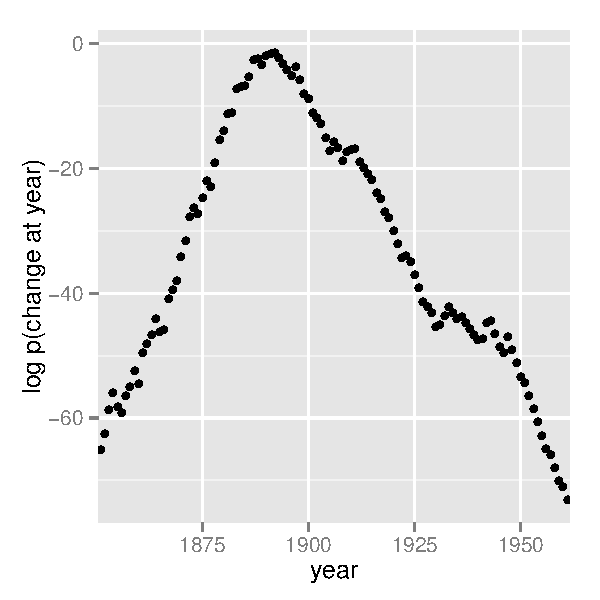
\includegraphics[height=2in]{img/change-point-posterior.pdf}
\ \ \ \ \
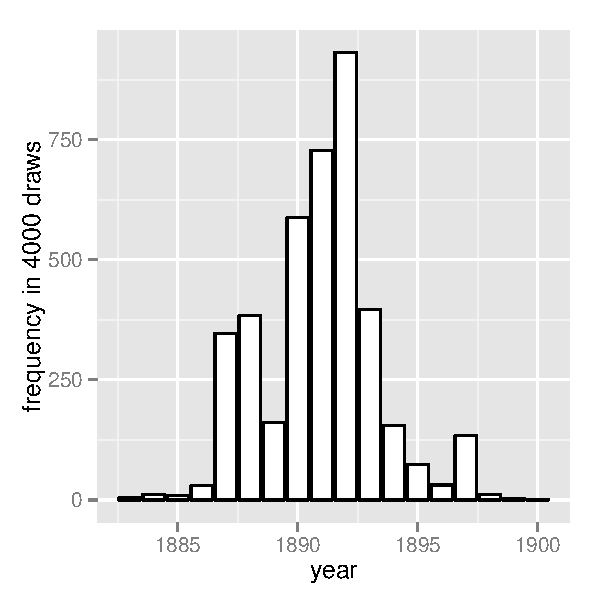
\includegraphics[height=2in]{img/s-discrete-posterior.pdf}
\end{center}
\vspace*{-12pt}
\caption{\small\it The posterior estimates for the change point.  \
  {\rm Left)} log probability of change point being in year,
  calculated analytically using \code{lp}; \ {\rm Right)}\ frequency
  of change point draws in the posterior generated using
  \code{lp}. The plot on the left is on the log scale and the plot on
  the right on the linear scale; note the narrower range of years in
  the right-hand plot resulting from sampling. The posterior mean of
  $s$ is roughly 1891.}%
\label{change-point-posterior.figure}
\end{figure}
%



\subsection{Discrete Sampling}

Although not computationally advantageous compared to working in
expectation using \code{lp}, it is possible to use Stan to sample the
value of \code{s} at every iteration.
%
\begin{quote}
\begin{Verbatim}
generated quantities {
  int<lower=1,upper=T> s;
  s <- categorical_rng(softmax(lp));
}
\end{Verbatim}
\end{quote}
%
A posterior histogram of draws for $s$ is shown on the right side of
\reffigure{change-point-posterior}.


\subsection{Posterior Covariance}

The discrete sample generated for $s$ can be used to calculate
covariance with other parameters.  Although the sampling approach is
straightforward, it is more statistically efficient (in the sense of
requiring far fewer iterations for the same degree of accuracy) to
calculate these covariances in expectation using \code{lp}.




\section{Mark-Recapture Models}

A widely applied field method in ecology is to capture (or sight)
animals, mark them (e.g., by tagging), then release them.  This
process is then repeated one or more times, and is often done for
populations on an ongoing basis.  The resulting data may be used to
estimate population size.

The first subsection describes a very simple mark-recapture model that does
not involve any latent discrete parameters.  The following subsections
describes the Cormack-Jolly-Seber model, which involves latent
discrete parameters for animal death.

\subsection{Simple Mark-Recapture Model}

In the simplest case, a one-stage mark-recapture study produces the
following data
%
\begin{itemize}
\item $M$ : number of animals marked in first capture,
\item $C$ : number animals in second capture, and
\item $R$ : number of marked animals in second capture.
\end{itemize}
%
The estimand of interest is
%
\begin{itemize}
\item $N$ : number of animals in the population.
\end{itemize}
%
Despite the notation, the model will take $N$ to be a continuous
parameter; just because the population must be finite doesn't mean the
parameter representing it must be.  The parameter will be used to
produce a real-valued estimate of the population size.

The Lincoln-Petersen \citep{Lincoln:1930,Petersen:1896} method for
estimating population size is
%
\[
\hat{N} = \frac{M C}{R}.
\]
%
This population estimate would arise from a probabilistic model in
which the number of recaptured animals is distributed binomially,
\[
R \sim \distro{Binomial}(C, M / N)
\]
given the total number of animals captured in the second round ($C$)
with a recapture probability of $M/N$, the fraction of the total
population $N$ marked in the first round.

%
\begin{figure}
\begin{quote}\small
\begin{Verbatim}
data {
  int<lower=0> M;
  int<lower=0> C;
  int<lower=0,upper=min(M,C)> R;
}
parameters {
  real<lower=(C - R + M)> N;
}
model {
  R ~ binomial(C, M / N);
}
\end{Verbatim}
\end{quote}
\vspace*{-6pt}
\caption{\small\it A probabilistic formulation of the Lincoln-Petersen
population estimator for pulation size based on data from a one-step
mark-recapture study.  The lower bound on $N$ is necessary to
efficiently eliminate impossible values.}%
\label{lincoln-petersen-model.figure}
\end{figure}
%
The probabilistic variant of the Lincoln-Petersen estimator can be
directly coded in Stan as shown in \reffigure{lincoln-petersen-model}.
The Lincoln-Petersen estimate is the maximum likelihood estimate (MLE)
for this model.

To enusre the MLE is the Lincoln-Petersen estimate, an improper
uniform prior for $N$ is used; this could (and should) be replaced
with a more informative prior if possible based on knowledge of the
population under study.

The one tricky part of the model is the lower bound $C - R + M$ placed
on the population size $N$.  Values below this bound are impossible
because it is otherwise not possible to draw $R$ samples out of the
$C$ animals recaptured.  Implementing this lower bound is necessary to
ensure sampling and optimization can be carried out in an
unconstrained manner with unbounded support for parameters on the
transformed (unconstrained) space.  The lower bound in the declaration
for $C$ implies a variable transform $f : (C-R+M,\infty) \rightarrow
(-\infty,+\infty)$ defined by $f(N) = \log(N - (C - R + M))$; see
\refsection{lower-bound-transform} for more information on the
transform used for variables declared with a lower bound.

\subsection{Cormack-Jolly-Seber with Discrete Parameter}

The Cormack-Jolly-Seber (CJS) model
\citep{Cormack:1964,Jolly:1965,Seber:1965} is an open-population model
in which the population may change over time due to death; the
presentation here draws heavily on \citep{Schofield:2007}.  

The basic data is
%
\begin{itemize}
\item $I$ : number of individuals, 
\item $T$ : number of capture periods, and
\item $y_{i,t}$ : boolean indicating if individual $i$ was captured at
  time $t$.
\end{itemize}
%
Each individual is assumed to have been captured at least once because
an individual only contributes information conditionally after they
have been captured the first time.

There are two Bernoulli parameters in the model,
%
\begin{itemize}
\item $\phi_t$ : probability that animal alive at time $t$ survives
  until $t + 1$ and
\item $p_t$ : probability that animal alive at time $t$ is captured at
  time $t$.
\end{itemize}
%
These parameters will both be given uniform priors, but information
should be used to tighten these priors in practice.

The CJS model also employs a latent discrete parameter $z_{i,t}$
indicating for each individual $i$ whether it is alive at time $t$,
distributed as
%
\[
z_{i,t} \sim \distro{Bernoulli}(\ternary{z_{i,t-1}}{0}{\phi_{t-1}}).
\]
%
The conditional prevents the model positing zombies; once an animal is
dead, it stays dead.  The data distribution is then simple to express
conditional on $z$ as
%
\[
y_{i,t} \sim \distro{Bernoulli}(\ternary{z_{i,t}}{0}{p_t})
\]
%
The conditional enforces the constraint that dead animals cannot be captured.


\subsection{Collective Cormack-Jolly-Seber Model}

This subsection presents an implementation of the model in terms of
counts for different history profiles for individuals over three
capture times. It assumes exchangeability of the animals in that each
is assigned the same capture and survival probabilities.

In order to ease the marginalization of the latent discrete parameter
$z_{i,t}$, the Stan models rely on a derived quantity $\chi_t$ for
the probability that an individual is never captured again if it is
alive at time $t$ (if it is dead, the recapture probability is zero).
this quantity is defined recursively by
\[
\chi_t 
= 
\begin{cases}
1 
& \mbox{if } t = T
\\[3pt]
(1 - \phi_t) + \phi_t (1 - p_{t+1}) \chi_{t+1}
& \mbox{ if } t < T
\end{cases}
\]
%
The base case arises because if an animal was captured in the last
time period, the probability it is never captured again is 1 because
there are no more capture periods.  The recursive case defining
$\chi_{t}$ in terms of $\chi_{t+1}$ involves two possibiliites: (1)
not surviving to the next time period, with probability $(1 -
\phi_t)$, or (2) suriviving to the next time period with probability
$\phi_t$, not being captured in the next time period with probabilty
$(1 - p_{t+1})$, and not being captured again after being alive in
period $t+1$ with probability $\chi_{t+1}$. 

With three capture times, there are three captured/not-captured
profiles an individual may have.  These may be naturally coded as
binary numbers as follows.
%
\begin{center}
\begin{tabular}{c|ccc|c}
& \multicolumn{3}{|c|}{{\it captures}}
\\
{\it profile} & 1 & 2 & 3 & {\it probability}
\\ \hline
{0} & - & - & - & n/a
\\
{1} & - & - & + & n/a
\\ \hline
{2} & - & + & - & $\chi_2$
\\
{3} & - & + & + & $\phi_2 \, \phi_3$
\\ \hline
{4} & + & - & - & $\chi_1$
\\
{5} & + & - & + & $\phi_1 \, (1 - p_2) \, \phi_2 \, p_3$
\\ \hline
{6} & + & + & - & $ \phi_1 \, p_2 \, \chi_2$
\\ 
{7} & + & + & + & $\phi_1 \, p_2 \, \phi_2 \, p_3$
\end{tabular}
\end{center}
%
History 0, for animals that are never captured, is unobservable
because only animals that are captured are observed. History 1, for
animals that are only captured in the last round, provides no
information for the CJS model, because capture/non-capture status is
only informative when conditioned on earlier captures.  For the
remaining cases, the contribution to the likelihood is provided in the
final column.

By defining these probabilities in terms of $\chi$ directly, there is
no need for a latent binary parameter indicating whether an animal is
alive at time $t$ or not.  The definition of $\chi$ is typically used
to define the likelihood (i.e., marginalize out the latent discrete
parameter) for the CJS model \citep[page 9]{Schofield:2007}.

The Stan model defines $\chi$ as a transformed parameter based on
parameters $\phi$ and $p$.  In the model block, the log probability is
incremented for each history based on its count.  This second step is
similar to collecting Bernoulli observations into a binomial or
categorical observations into a multinomial, only it is coded directly
in the Stan program using \code{increment\_log\_prob} rather than
being part of a built-in probability function.
%
\begin{figure}
\begin{quote}\small
\begin{Verbatim}
data {
  int<lower=0> history[7];
}
parameters {
  real<lower=0,upper=1> phi[2];
  real<lower=0,upper=1> p[3];
}
transformed parameters {
  real<lower=0,upper=1> chi[2];  
  chi[2] <- (1 - phi[2]) + phi[2] * (1 - p[3]);
  chi[1] <- (1 - phi[1]) + phi[1] * (1 - p[2]) * chi[2];
}
model {
  increment_log_prob(history[2] * log(chi[2]));
  increment_log_prob(history[3] * (log(phi[2]) + log(p[3])));
  increment_log_prob(history[4] * (log(chi[1])));
  increment_log_prob(history[5] 
                     * (log(phi[1]) + log1m(p[2])
                        + log(phi[2]) + log(p[3])));
  increment_log_prob(history[6] 
                     * (log(phi[1]) + log(p[2]) 
                        + log(chi[2])));
  increment_log_prob(history[7] 
                     * (log(phi[1]) + log(p[2]) 
                        + log(phi[2]) + log(p[3])));
}
generated quantities {
  real<lower=0,upper=1> beta3;
  beta3 <- phi[2] * p[3];
}
\end{Verbatim}
\end{quote}
\vspace*{-12pt}
\caption{\small\it A Stan program for the Cormack-Jolly-Seber
  mark-recapture model that considers counts of individuals with
  observation histories of being observed or not in three capture
  periods.}\label{cjs-history.figure}
\end{figure}
%

\subsubsection{Identifiability}

The parameters $\phi_2$ and $p_3$, the probability of death at time 2
and probabilty of capture at time 3 are not identifiable, because both
may be used to account for lack of capture at time 3.  Their product,
$\beta_3 = \phi_2 \, p_3$, is identified.  The Stan model defines
\code{beta3} as a generated quantity.  Unidentified parameters pose a
problem for Stan's samplers' adaptation.  Although the problem posed
for adaptation is mild here because the parameters are bounded and
thus have proper uniform priors, it would be better to formulate an
identified parameterization.  One way to do this would be to formulate
a hierarchical model for the $p$ and $\phi$ parameters.

\subsection{Individual Cormack-Jolly-Seber Model}

This section presents a version of the Cormack-Jolly-Seber (CJS) model
cast at the individual level rather than collectively as in the
previous subsection.  It also extends the model to allow an arbitrary
number of time periods.  The data will consist of the number $T$ of
capture events, the number $I$ of individuals, and a boolean flag
$y_{i,t}$ indicating if individual $i$ was observed at time $t$.  In
Stan,
%
\begin{quote}
\begin{Verbatim}
data {
  int<lower=2> T;
  int<lower=0> I;
  int<lower=0,upper=1> y[I,T];
}
\end{Verbatim}
\end{quote}

The advantages to the individual-level model is that it becomes
possible to add individual ``random effects'' that affect survival or
capture probability, as well as to avoid the combinatorics involved in
unfolding $2^T$ observation histories for $T$ capture times.

\subsubsection{Utility Functions}

The individual CJS model is written involves several function
definitions.  The first two are used in the transformed data block to
compute the first and last time period in which an animal was
captured.%
%
\footnote{An alternative would be to compute this on the outside and
feed it into the Stan model as preprocessed data.  Yet another
alternative encoding would be a sparse one recording only the
capture events along with their time and identifying the individual
captured.} 
%
\begin{quote}
\begin{Verbatim}
functions {
  int first_capture(int[] y_i) {
    for (k in 1:size(y_i))
      if (y_i[k])
        return k;
    return 0;
  }
  int last_capture(int[] y_i) { 
    for (k_rev in 0:(size(y_i) - 1)) {
      int k;
      k <- size(y_i) - k_rev;
      if (y_i[k]) 
        return k;
    }
    return 0;
  }
  ...
}
\end{Verbatim}
\end{quote}
%
These two functions are used to define the first and last capture time
for each individual in the transformed data block.%
%
\footnote{Both functions return 0 if the individual represented by the
  input array was never captured.  Individuals with no captures are
  not relevant for estimating the model because all probability
  statements are conditional on earlier captures.  Typically they
  would be removed from the data, but the program allows them to be
  included even though they make not contribution to the log
  probability function.}
%
\begin{quote}
\begin{Verbatim}
transformed data {
  int<lower=0,upper=T> first[I];
  int<lower=0,upper=T> last[I];
  vector<lower=0,upper=I>[T] n_captured;
  for (i in 1:I)
    first[i] <- first_capture(y[i]);
  for (i in 1:I)
    last[i] <- last_capture(y[i]);
  n_captured <- rep_vector(0,T);
  for (t in 1:T)
    for (i in 1:I)
      if (y[i,t]) 
        n_captured[t] <- n_captured[t] + 1;
}
\end{Verbatim}
\end{quote}
%
The transformed data block also defines \code{n\_captured[t]}, which is
the total number of captures at time \code{t}.  The variable
\code{n\_captured} is defined as a vector instead of an integer array
so that it can be used in an elementwise vector operation in the generated
quantities block to model the population estimates at each time point.

The parameters and transformed parameters are as before, but now there
is a function definition for computing the entire vector \code{chi}, the
probability that if an individual is alive at \code{t} that it will
never be captured again.
%
\begin{quote}
\begin{Verbatim}
parameters {
  vector<lower=0,upper=1>[T-1] phi;
  vector<lower=0,upper=1>[T] p;
}
transformed parameters {
  vector<lower=0,upper=1>[T] chi;
  chi <- prob_uncaptured(T,p,phi);
}
\end{Verbatim}
\end{quote}
%
The definition of \code{prob\_uncaptured}, from the functions block,
is
%
\begin{quote}
\begin{Verbatim}
funtions {
  ...
  vector prob_uncaptured(int T, vector p, vector phi) {
    vector[T] chi;
    chi[T] <- 1.0;              
    for (t in 1:(T - 1)) {
      int t_curr;
      int t_next;
      t_curr <- T - t;
      t_next <- t_curr + 1;
      chi[t_curr] <- (1 - phi[t_curr]) 
                     + phi[t_curr] 
                       * (1 - p[t_next]) 
                       * chi[t_next]; 
    }
    return chi;
  }
}
\end{Verbatim}
\end{quote}
%
The function definition directly follows the mathematical definition
of $\chi_t$, unrolling the recursion into an iteration and
defining the elements of \code{chi} from \code{T} down to 1.

\subsubsection{The Model}

Given the precomputed quantities, the model block directly encodes the
CJS model's log likelihood function.  All parameters are left with
their default uniform priors and the model simply encodes the log
probability of the observations \code{q} given the parameters \code{p}
and \code{phi} as well as the transformed parameter \code{chi} defined
in terms of \code{p} and \code{phi}.
%
\begin{quote}
\begin{Verbatim}
model {
  for (i in 1:I) {
    if (first[i] > 0) {
      for (t in (first[i]+1):last[i]) {
        1 ~ bernoulli(phi[t-1]);
        y[i,t] ~ bernoulli(p[t]);
      }
      1 ~ bernoulli(chi[last[i]]);
    }
  }
}
\end{Verbatim}
\end{quote}
%
The outer loop is over individuals, conditional skipping individuals
\code{i} which are never captured.  The never-captured check depends
on the convention of the first-capture and last-capture functions
returning 0 for \code{first} if an individual is never captured.

The inner loop for individual \code{i} first increments the log
probability based on the survival of the individual with proability
\code{phi[t-1]}.  The outcome of 1 is fixed because the individual
must survive between the first and last capture (i.e., no zombies).
Note that the loop starts after the first capture, because all
information in the CJS model is conditional on the first capture.

In the inner loop, the observed capture status \code{y[i,t]} for
individual \code{i} at time \code{t} has a Bernoulli distribution
based on the capture probabilty \code{p[t]} at time \code{t}.

After the inner loop, the probability of an animal never being seen
again after being observed at time \code{last[i]} is included, because
\code{last[i]} was defined to be the last time period in which animal
\code{i} was observed.

\subsubsection{Identified Parameters}

As with the collective model described in the previous subsection,
this model does not identify \code{phi[T-1]} and \code{p[T]}, but
does identify their product, \code{beta}.  Thus \code{beta} is defined
as a generated quantity to monitor convergence and report.
%
\begin{quote}
\begin{Verbatim}
generated quantities {
  real beta;
  ...

  beta <- phi[T-1] * p[T];
  ...
}
\end{Verbatim}
\end{quote}
%

The parameter \code{p[1]} is also not modeled and will just be uniform
between 0 and 1.  A more finely articulated model might have a
hierarchical or time-series component, in which case \code{p[1]} would
be an unknown intial condition and both \code{phi[T-1]} and
\code{p[T]} could be identified.

\subsubsection{Population Size Estimates}

The generated quantities also calculates an estimate of the population
mean at each time \code{t} in the same way as in the simple
mark-recapture model as the number of individuals captured at time
\code{t} divided by the probability of capture at time \code{t}.  This
is done with the elementwise division operation for vectors
(\code{./}) in the generated quantities block.
%
\begin{quote}
\begin{Verbatim}
generated quantities {
  ...
  vector<lower=0>[T] pop;
  ...
  pop <- n_captured ./ p;
  pop[1] <- -1;
}
\end{Verbatim}
\end{quote}

\subsubsection{Generalizing to Individual Effects}

All individuals are modeled as having the same capture probability,
but this model could be easily generalized to use a logistic
regression here based on individual-level inputs to be used as
predictors.



\section{Data Coding and Diagnostic Accuracy Models}

Although seemingly disparate tasks, the rating/coding/annotation of
items with categories and diagnostic testing for disease or other
conditions share several characteristics which allow their statistical
properties to modeled similarly.

\subsection{Diagnostic Accuracy}

Suppose you have diagnostic tests for a condition of varying
sensitivity and specificity.  Sensitivity is the probability a test
returns positive when the patient has the condition and specificity is
the probability that a test returns negative when the patient does not
have the condition.  For example, mammograms and puncture biopsy tests
both test for the presence of breast cancer.  Mammograms have high
sensitivity and low specificity, meaning lots of false positives,
whereas puncture biopsies are the opposite, with low sensitivity and
high specificity, meaning lots of false negatives.

There are several estimands of interest in such studies.  An
epidemiological study may be interested in the prevalence of a kind of
infection, such as malaria, in a population.  A test development study
might be interested in the diagnostic accuracy of a new test. A health
care worker performing tests might be interested in the disease status
of a particular patient.

\subsection{Data Coding}

Humans are often given the task of coding (equivalently rating or
annotating) data.  For example, journal or grant reviewers rate
submissions, a political study may code campaign commercials as to
whether they are attack ads or not, a natural language processing
study might annotate Tweets as to whehter they are positive or
negative in overall sentiment, or a dentist looking at an X-ray
classifies a patient as having a cavity or not.  In all of these
cases, the data coders play the role of the diagnostic tests and all
of the same estimands are in play --- data coder accuracy and bias,
true categories of items being coded, or the prevalence of various
categories of items in the data.

\subsection{Noisy Categorical Measurement Model}

In this section, only categorical ratings are considered, and the
challenge in the modeling for Stan is to marginalize out the discrete
parameters.  

\cite{DawidSkene:1979} introduce a noisy-measurement model for
data coding and apply in the epidemiological setting of coding what
doctor notes say about patient histories;  the same model can be used
for diagnostic procedures.

\subsubsection{Data}

The data for the model consists of $J$ raters (diagnostic tests), $I$
items (patients), and $K$ categories (condition statuses) to annotate,
with $y_{i,j} \in 1{:}K$ being the rating provided by rater $j$ for
item $i$.  In a diagnostic test setting for a particular condition,
the raters are diagnostic procedures and often $K=2$, with values
signaling the presense or absence of the condition.%
%
\footnote{Diagnostic procedures are often ordinal, as in stages of
  cancer in oncological diagnosis or the severity of a cavity in
  dental diagnosis.  Dawid and Skene's model may be used as is or
  naturally generalized for ordinal ratings using a latent continuous
  rating and cutpoints as in ordinal logistic regression.}

It is relatively straightforward to extend Dawid and Skene's model to
deal with the situation where not every rater rates each item exactly
once.

\subsection{Model Parameters}

The model is based on three parameters, the first of which is discrete:
%
\begin{itemize}
\item $z_i$ : a value in $1{:}K$ indicating the true category of item $i$,
\item $\pi$ : a $K$-simplex for the prevalence of the $K$
  categories in the population, and
\item $\theta_{j,k}$ : a $K$-simplex for the response of annotator $j$
  to an item of true category $k$.
\end{itemize}

\subsection{Noisy Measurement Model}

The true category of an item is assumed to be generated by a simple
categorical distribution based on item prevalence,
\[
z_i \sim \distro{Categorical}(\pi).
\]
%
The rating $y_{i,j}$ provided for item $i$ by rater $j$ is modeled as
a categorical response of rater $i$ to an item of category $z_i$,%
%
\footnote{In the subscript, $z[i]$ is written as $z_i$ to
  improve legibility.}
%
\[
y_{i,j} \sim \distro{Categorical}(\theta_{j,\pi_{z[i]}}).
\]

\subsubsection{Priors and Hierarchical Modeling}

Dawid and Skene provided maximum likelihood estimates for $\theta$ and
$\pi$, which allows them to generate probabilty estimates for each $z_i$.

To mimic Dawid and Skene's maximum likelihood model, the parameters
$\theta_{j,k}$ and $\pi$ can be given uniform priors over
$K$-simplexes.  It is straightforward to generalize to Dirichlet
priors,
\[
\pi \sim \distro{Dirichlet}(\alpha)
\]
and
\[
\theta_{j,k} \sim \distro{Dirichlet}(\beta_k)
\]
with fixed hyperparameters $\alpha$ and $\beta$.  The prior for
$\theta_{j,k}$ must be allowed to vary in $k$, so that, for instance,
$\beta_{k,k}$ is large enough to allow the prior to favor
better-than-chance annotators over random or adversarial ones.

Because there are $J$ coders, it would be natural to extend the model
to include a hierarchical prior for $\beta$ and to partially pool the
estimates of coder accuracy and bias.

\subsubsection{Marginalizing out the True Category}

Because the true category parameter $z$ is discrete, it must be
marginalized out of the joint posterior in order to carry out sampling
or maximum likelihood estimation in Stan. The joint posterior factors
as
\[
p(y, \theta, \pi) = p(y | \theta,\pi) \, p(\pi) \, p(\theta),
\]
where $p(y | \theta,\pi)$ is derived by marginalizing $z$ out of
%
\[
p(z, y | \theta, \pi)
\ = \
\prod_{i=1}^I \left( \distro{Categorical}(z_i | \pi)
                     \prod_{j=1}^J
                     \distro{Categorical}(y_{i,j}|\theta_{j,z[i]})
              \right).
\]
%
This can be done item by item, with
\[
p(y | \theta, \pi)
\ = \
\prod_{i=1}^I \sum_{k=1}^K  
  \left( \distro{Categorical}(z_i | \pi)
         \prod_{j=1}^J
         \distro{Categorical}(y_{i,j}|\theta_{j,z[i]})
  \right).
\]            
%
In the missing data model, only the observed labels would be used in
the inner product.

\cite{DawidSkene:1979} derive exactly the same equation in their
Equation~(2.7), required for the E-step in their expectation
maximization (EM) algorithm.  Stan requires the marginalized
probability function on the log scale,
\[
\begin{array}{l}
\mbox{ } \ \log p(y | \theta, \pi)
\\[3pt]
\mbox{ } \ \ \ = \
\sum_{i=1}^I \log \left( \sum_{k=1}^K \exp
  \left( \log \distro{Categorical}(z_i | \pi)
         + \sum_{j=1}^J
         \log \distro{Categorical}(y_{i,j}|\theta_{j,z[i]})
  \right) \right),
\end{array}
\]                            
which can be directly coded using Stan's built-in \code{log\_sum\_exp}
function.


\subsection{Stan Implementation}

The Stan program for the Dawid and Skene model is provided in
\reffigure{dawid-skene-model}.
%
\begin{figure}
\begin{quote}\small
\begin{Verbatim}
data {
  int<lower=2> K;
  int<lower=1> I;
  int<lower=1> J;

  int<lower=1,upper=K> y[I,J];

  vector<lower=0>[K] alpha;
  vector<lower=0>[K] beta[K];
}
parameters {
  simplex[K] pi;
  simplex[K] theta[J,K];
}
transformed parameters {
  vector[K] log_q_z[I];
  for (i in 1:I) {
    log_q_z[i] <- log(pi);
    for (j in 1:J)
      for (k in 1:K)
        log_q_z[i,k] <- log_q_z[i,k] 
                        + log(theta[j,k,y[i,j]]);
  }
}
model {
  pi ~ dirichlet(alpha);
  for (j in 1:J)
    for (k in 1:K)
      theta[j,k] ~ dirichlet(beta[k]);

  for (i in 1:I)
    increment_log_prob(log_sum_exp(log_q_z[i]));
}
\end{Verbatim}
\end{quote}
\vspace*{-12pt}
\caption{\small\it Stan program for the rating (or diagnostic
  accuracy) model of \cite{DawidSkene:1979}. The model marginalizes
  out the discrete parameter $z$, storing the unnormalized conditional
  probability $\log q(z_i=k|\theta,\pi)$ in\ \code{log\_q\_z[i,k]}.}%
\label{dawid-skene-model.figure}
\end{figure}
%
The Stan model converges quickly and mixes well using NUTS starting at
diffuse initial points, unlike the equivalent model implemented with
Gibbs sampling over the discrete parameter.  Reasonable weakly
informative priors are $\alpha_k = 3$ and $\beta_{k,k} = 2.5 K$ and
$\beta_{k,k'} = 1$ if $k \neq k'$.  Taking $\alpha$ and $\beta_k$ to
be unit vectors and applying optimization will produce the same answer
as the expectation maximization (EM) algorithm of
\cite{DawidSkene:1979}.  

\subsubsection{Inference for the True Category}

The quantity \code{log\_q\_z[i]} is defined as a transformed
parameter.  It encodes the (unnormalized) log of $p(z_i | \theta,
\pi)$.  Each iteration provides a value conditioned on that
iteration's values for $\theta$ and $\pi$.  Applying the softmax
function to \code{log\_q\_z[i]} provides a simplex corresponding to
the probability mass function of $z_i$ in the posterior.   These may
be averaged across the iterations to provide the posterior probability
distribution over each $z_i$.


\chapter{Clustering Models}\label{clustering.chapter}

\noindent
Unsupervised methods for organizing data into groups are collectively
referred to as clustering.  This chapter describes the implementation
in Stan of two widely used statistical clustering models, soft
$K$-means and latent Dirichlet allocation (LDA).  In addition, this
chapter includes naive Bayesian classification, which can be viewed as
a form of clustering which may be supervised.  These models are
typically expressed using discrete parameters for cluster assignments.
Nevertheless, they can be implemented in Stan like any other mixture
model by marginalizing out the discrete parameters (see
\refchapter{mixture-modeling}).

\section{Soft $K$-Means}

$K$-means clustering is a method of clustering data represented as
$D$-dimensional vectors.  Specifically, there will be $N$ items to be
clustered, each represented as a vector $y_n \in \reals^D$.  In the
``soft'' version of $K$-means, the assignments to clusters will be
probabilistic.  

\subsection{Geometric Hard  $K$-Means Clustering}

$K$-means clustering is typically described geometrically in terms of
the following algorithm, which assumes the number of clusters $K$ and
data vectors $y$ as input.
%
\begin{enumerate}
\item For each $n$ in $1:N$, randomly assign vector $y_n$ to a cluster in $1{:}K$;
\item Repeat
\begin{enumerate} 
\item For each cluster $k$ in $1{:}K$, compute the cluster centroid $\mu_k$  by averaging the
  vectors assigned to that cluster;
\item For each $n$ in $1:N$, reassign $y_n$ to the cluster $k$ to
  for which the (Euclidean) distance from $y_n$ to $\mu_k$ is smallest;
\item If no vectors changed cluster, return the cluster assignments.
\end{enumerate}
\end{enumerate}
%
This algorithm is guaranteed to terminate.

\subsection{Soft $K$-Means Clustering}

Soft $K$-means clustering treats the cluster assignments as
probability distributions over the clusters.  Because of the
connection between Euclidean distance and multivariate normal models
with a fixed covariance, soft $K$-means can be expressed (and coded in
Stan) as a multivariate normal mixture model.

In the full generative model, each data point $n$ in $1{:}N$ is assigned
a cluster $z_n \in 1{:}K$ with symmetric uniform probability,
%
\[
z_n \sim \distro{Categorical}({\bf 1}/K),
\]
where ${\bf 1}$ is the unit vector of $K$ dimensions, so that ${\bf
  1}/K$ is the symmetric $K$-simplex.  Thus the model assumes that
each data point is drawn from a hard decision about cluster
membership.  The softness arises only from the uncertainty about which
cluster generated a data point.

The data points themselves are generated from a multivariate normal
distribution whose parameters are determined by the cluster assignment
$z_n$,
\[
y_n \sim  \distro{Normal}(\mu_{z[n]},\Sigma_{z[n]})
\]

The sample implementation in this section assumes a fixed unit
covariance matrix shared by all clusters $k$,
\[
\Sigma_k = \mbox{diag\_matrix}({\bf 1}),
\]
so that the log multivariate normal can be implemented directly up to a proportion
by
\[
\mbox{Normal}\left( y_n | \mu_k, \mbox{diag\_matrix}({\bf 1}) \right)
\propto \exp \left (- \frac{1}{2} \sum_{d=1}^D \left( \mu_{k,d} - y_{n,d}
  \right)^2 \right).
\]
The spatial perspective on $K$-means arises by noting that the inner
term is just half the negative Euclidean distance from the cluster
mean $\mu_k$ to the data point $y_n$.

\subsection{Stan Implementation of Soft $K$-Means}

The following model is available in the Stan distribution (along with
an R program to randomly generate data sets and a sample data set) in
the directory \nolinkurl{stan/example-models/misc/soft-k-means}.
%
\begin{quote}
\begin{Verbatim}[fontsize=\small]
data {
  int<lower=0> N;  // number of data points
  int<lower=1> D;  // number of dimensions
  int<lower=1> K;  // number of clusters
  vector[D] y[N];  // observations
}
transformed data {
  real<upper=0> neg_log_K;
  neg_log_K <- -log(K);
}
parameters {
  vector[D] mu[K]; // cluster means
}
transformed parameters {
  real<upper=0> soft_z[N,K]; // log unnormalized clusters
  for (n in 1:N)
    for (k in 1:K)
      soft_z[n,k] <- neg_log_K 
                     - 0.5 * dot_self(mu[k] - y[n]);
}
model {
  // prior
  for (k in 1:K)
    mu[k] ~ normal(0,1);

  // likelihood
  for (n in 1:N)
    increment_log_prob(log_sum_exp(soft_z[n])); 
}
\end{Verbatim}
\end{quote}
%
There is an independent unit normal prior on the centroid parameters;
this prior could be swapped with other priors, or even a hierarchical
model to fit an overall problem scale and location.

The only parameter is \code{mu}, where \code{mu[k]} is the centroid
for cluster $k$.  The transformed parameters \code{soft\_z[n]} contain
the log of the unnormalized cluster assignment probabilities.  The
vector \code{soft\_z[n]} can be converted back to a normalized simplex
using the softmax function (see \refsection{softmax}), either externally
externally or within the model's generated quantities block.

\subsection{Generalizing Soft $K$-Means}

The multivariate normal distribution with unit covariance matrix
produces a log probability density proportional to Euclidean distance
(i.e., $L_2$ distance).  Other distributions relate to other
geometries.  For instance, replacing the normal distribution with the
double exponential (Laplace) distribution produces a clustering model
based on $L_1$ distance (i.e., Manhattan or taxicab
distance). 

Within the multivariate normal version of $K$-means, replacing the
unit covariance matrix with a shared covariance matrix amounts to
working with distances defined in a space transformed by the inverse
covariance matrix.

Although there is no global spatial analog, it is common to see soft
$K$-means specified with a per-cluster covariance matrix. In this
situation, a hierarchical prior may be used for the covariance matrices.



\section{The Difficulty of Bayesian Inference for Clustering}

Two problems make it pretty much impossible to perform full Bayesian
inference for clustering models, the lack of parameter identifiability
and the extreme multimodality of the posteriors.  There is additional
discussion related to the non-identifiability due to label swtiching
in \refsection{label-switching-problematic}.

\subsection{Non-Identifiability}

Cluster assignments are not identified --- permuting the cluster mean
vectors \code{mu} leads to a model with identical likelihoods.  For
instance, permuting the first two indexes in \code{mu} and the first
two indexes in each \code{soft\_z[n]} leads to an identical likelihood
(and prior).

The lack of identifiability means that the the cluster parameters
cannot be compared across multiple Markov chains.  In fact, the only
parameter in soft $K$-means is not identified, leading to problems in
monitoring convergence.  Clusters can even fail to be identified
within a single chain, with indices swapping if the chain is long
enough or the data is not cleanly separated. 

\subsection{Multimodality}

The other problem with clustering models is that their posteriors are
highly multimodal.  One form of multimodality is the
non-identifiability leading to index swapping.  But even without
the index problems the posteriors are highly mulitmodal.

Bayesian inference fails in cases of high multimodality because there
is no way to visit all of the modes in the posterior in appropriate
proportions and thus no way to evaluate integrals involved in
posterior predictive inference.

In light of these two problems, the advice often given in fitting
clustering models is to try many different initializations and select
the sample with the highest overall probability.  It is also popular
to use optimization-based point estimators such as expectation
maximization or variational Bayes, which can be much more efficient
than sampling-based approaches.


\section{Naive Bayes Classification and Clustering}

Naive Bayes is a kind of mixture model that can be used for
classification or for clustering (or a mix of both), depending on
which labels for items are observed.%
%
\footnote{For clustering, the non-identifiability problems for all
  mixture models present a problem, whereas there is no such problem
  for classification.  Despite the difficulties with full Bayesian
  inference for clustering, researchers continue to use it, often in
  an explorata data analysis setting rather than for predictive
  modeling.}

Multinomial mixture models are referred to as ``naive Bayes'' because
they are often applied to classification problems where the
multinomial independence assumptions are clearly false. 

Naive Bayes classification and clustering can be applied to any data
with multinomial structure.  A typical example of this is natural
language text classification and clustering, which is used an example
in what follows. 

The observed data consists of a sequence of $M$ documents made up of
bags of words drawn from a vocabulary of $V$ distinct words.  A
document $m$ has $N_m$ words, which are indexed as $w_{m,1}, \ldots,
w_{m,N[m]} \in 1{:}V$.  Despite the ordered indexing of words in a
document, this order is not part of the model, which is clearly
defective for natural human language data.  A number of topics (or
categories) $K$ is fixed.

The multinomial mixture model generates a single category $z_m \in
1{:}K$ for each document $m \in 1{:}M$ according to a categorical
distribution,
\[
z_m \sim \distro{Categorical}(\theta).
\]
The $K$-simplex parameter $\theta$ represents the prevalence of each
category in the data.  

Next, the words in each document are generated conditionally
independently of each other and the words in other documents based on
the category of the document, with word $n$ of document $m$ being
generated as
\[
w_{m,n} \sim \distro{Categorical}(\phi_{z[m]}).
\]
The parameter $\phi_{z[m]}$ is a $V$-simplex representing the
probability of each word in the vocabulary in documents of category
$z_m$.

The parameters $\theta$ and $\pi$ are typically given symmetric
Dirichlet priors.  The prevalence $\theta$ is sometimes fixed to
produce equal probabilities for each category $k \in 1:K$.

\subsection{Representing Ragged Arrays in Stan}

The specification for naive Bayes in the previous sections have used a ragged
array notation for the words $w$.  Because Stan does not support
ragged arrays, the models are coded using an alternative strategy that
provides an index for each word in a global list of words.   The data
is organized as follows, with the word arrays layed out in a column and each
assigned to its document in a second column.
%
\begin{center}
\begin{tabular}{r|cc}
\code{n} & \code{w[n]} & \code{doc[n]} \\ \hline
1 & $w_{1,1}$ & 1 \\
2 & $w_{1,2}$ & 1 \\
\vdots & \vdots & \vdots \\
$N_1$ & $w_{1,N[1]}$ & 1 \\
$N_1 + 1$ & $w_{2,1}$ & 2 \\
$N_1 + 2$ & $w_{2,2}$ & 2 \\
\vdots & \vdots & \vdots \\
$N_1 + N_2$ & $w_{2,N[2]}$ & 2 \\
$N_1 + N_2 + 1$ & $w_{3,1}$ & 3 \\
\vdots & \vdots & \vdots \\
$\code{N} = \sum_{m=1}^M N_m$ & $w_{M,N[M]}$ & $M$ \\
\end{tabular}
\end{center}
%
The relevant variables for the program are \code{N}, the total number
of words in all the documents, the word array \code{w}, and the
document identity array \code{doc}.  

\subsection{Estimation with Category-Labeled Training Data}

The naive Bayes models along with R programs to simulate data for them
and a sample data set are available in the distribution in the
directory \nolinkurl{example-models/misc/clustering/naive-bayes}.

A naive Bayes model for estimating the simplex parameters given
training data with documents of known categories can be coded in Stan
as follows 
%
\begin{quote}
\begin{Verbatim}[fontsize=\small]
data {
  // training data
  int<lower=1> K;               // num topics
  int<lower=1> V;               // num words
  int<lower=0> M;               // num docs
  int<lower=0> N;               // total word instances
  int<lower=1,upper=K> z[M];    // topic for doc m
  int<lower=1,upper=V> w[N];    // word n
  int<lower=1,upper=M> doc[N];  // doc ID for word n
  // hyperparameters
  vector<lower=0>[K] alpha;     // topic prior
  vector<lower=0>[V] beta;      // word prior
}
parameters {
  simplex[K] theta;   // topic prevalence
  simplex[V] phi[K];  // word dist for topic k
}
model {
  theta ~ dirichlet(alpha);
  for (k in 1:K)  
    phi[k] ~ dirichlet(beta);
  for (m in 1:M)
    z[m] ~ categorical(theta);
  for (n in 1:N)
    w[n] ~ categorical(phi[z[doc[n]]]);
}
\end{Verbatim}
\end{quote}
%
Note that the topic identifiers $z_m$ are declared as data and the
latent category assignments are included as part of the likelihood
function.  

\subsection{Estimation without Category-Labeled Training Data}

Naive Bayes models can be used in an unsupervised fashion to cluster
multinomial-structured data into a fixed number $K$ of categories.  
The data declaration includes the same variables as the model in the
previous section excluding the topic labels \code{z}.   Because
\code{z} is discrete, it needs to be summed out of the model
calculation.  This is done for naive Bayes as for other mixture
models.  The parameters are the same up to the priors, but the
likelihood is now computed as the marginal document probability
\[
\begin{array}{l}
\log p(w_{m,1},\ldots,w_{m,N_m}|\theta,\phi)
\\[2pt]
\ \ \ = \ 
\log \sum_{k=1}^K 
\left( \distro{Categorical}(k|\theta)
        \times \prod_{n=1}^{N_m} \distro{Categorical}(w_{m,n}|\phi_k)
\right)
\\[6pt]
\ \ \ = \ 
\log \sum_{k=1}^K \exp \left(
\log \distro{Categorical}(k|\theta)
+ \sum_{n=1}^{N_m} \log \distro{Categorical}(w_{m,n}|\phi_k)
\right).
\end{array}
\]
%
The last step shows how the \code{log\_sum\_exp} function can be used
to stabilize the numerical calculation and return a result on the log
scale.
%
\begin{quote}
\begin{Verbatim}[fontsize=\small]
model {
  real gamma[M,K];
  theta ~ dirichlet(alpha);
  for (k in 1:K)
    phi[k] ~ dirichlet(beta);
  for (m in 1:M) 
    for (k in 1:K) 
      gamma[m,k] <- categorical_log(k,theta);
  for (n in 1:N)
    for (k in 1:K)
      gamma[doc[n],k] <- gamma[doc[n],k] 
                         + categorical_log(w[n],phi[k]);
  for (m in 1:M)
    increment_log_prob(log_sum_exp(gamma[m]));
}
\end{Verbatim}
\end{quote}
%
The local variable \code{gamma[m,k]} represents the value
\[
\gamma_{m,k} = \log \distro{Categorical}(k|\theta)
+ \sum_{n=1}^{N_m} \log \distro{Categorical}(w_{m,n}|\phi_k).
\]
%
Given $\gamma$, the posterior probability that document
$m$ is assigned category $k$ is
\[
\mbox{Pr}[z_m = k|w,\alpha,\beta]
=
\exp \left( 
\gamma_{m,k}
- \log \sum_{k=1}^K \exp \left( \gamma_{m,k} \right)
\right).
\]
%
If the variable \code{gamma} were declared and defined in the
transformed parameter block, its sampled values would be saved by
Stan.  The normalized posterior probabilities could also be defined as
generated quantities.

\subsection{Full Bayesian Inference for Naive Bayes}

Full Bayesian posterior predictive inference for the naive Bayes model
can be implemented in Stan by combining the models for labeled and
unlabeled data.  The estimands include both the model parameters and
the posterior distribution over categories for the unlabeled data.  The
model is essentially a missing data model assuming the unknown
category labels are missing completely at random; see
\citep{GelmanEtAl:2013,GelmanHill:2007} for more
information on missing data imputation.  The model is also an instance
of semisupervised learning because the unlabeled data contributes to
the parameter estimations.

To specify a Stan model for performing full Bayesian inference, the
model for labeled data is combined with the model for unlabeled data.
A second document collection is declared as data, but without the
category labels, leading to new variables \code{M2} \code{N2},
\code{w2}, \and \code{doc2}.  The number of categories and number of
words, as well as the hyperparameters are shared and only declared
once.  Similarly, there is only one set of parameters.  Then the model
contains a single set of statements for the prior, a set of statements
for the labeled data, and a set of statements for the unlabeled data.

\subsection{Prediction without Model Updates}

An alternative to full Bayesian inference involves estimating a model
using labeled data, then applying it to unlabeled data without
updating the parameter estimates based on the unlabeled data.  This
behavior can be implemented by moving the definition of \code{gamma}
for the unlabeled documents to the generated quantities block.
Because the variables no longer contribute to the log probability,
they no longer jointly contribute to the estimation of the model
parameters.


\section{Latent Dirichlet Allocation}

Latent Dirichlet allocation (LDA) is a mixed-membership multinomial
clustering model \citep{BleiNgJordan:2003} that generalized naive
Bayes.  Using the topic and document terminology common in discussions of
LDA, each document is modeled as having a mixture of topics, with each
word drawn from a topic based on the mixing proportions.

\subsection{The LDA Model}

The basic model assumes each document is generated independently based
on fixed hyperparameters. For document $m$, the first step is to draw a topic
distribution simplex $\theta_m$ over the $K$ topics,
%
\[
\theta_m \sim \distro{Dirichlet}(\alpha).
\]
%
The prior hyperparameter $\alpha$ is fixed to a $K$-vector of positive
values.  Each word in the document is generated independently
conditional on the distribution $\theta_m$.  First, a topic
$z_{m,n} \in 1{:}K$ is drawn for the word based on the
document-specific topic-distribution,
\[
z_{m,n} \sim \distro{Categorical}(\theta_m).
\]
%
Finally, the word $w_{m,n}$ is drawn according to the word distribution
for topic $z_{m,n}$,
\[
w_{m,n} \sim \distro{Categorical}(\phi_{z[m,n]}).
\]
The distributions $\phi_k$ over words for topic $k$ are also given a
Dirichlet prior,
\[
\phi_k \sim \distro{Dirichlet}(\beta)
\]
%
where $\beta$ is a fixed $V$-vector of positive values.

\subsection{Summing out the Discrete Parameters}

Although Stan does not (yet) support discrete sampling, it is possible
to calculate the marginal distribution over the continuous parameters
by summing out the discrete parameters as in other mixture models.
The marginal posterior of the topic and word variables is
%
\begin{eqnarray*}
p(\theta,\phi|w,\alpha,\beta)
& \propto & 
p(\theta|\alpha) \times p(\phi|\beta) \times p(w|\theta,\phi)
\\[4pt]
& = & 
\prod_{m=1}^M p(\theta_m|\alpha)
\times
\prod_{k=1}^K p(\phi_k|\beta)
\times
\prod_{m=1}^M \prod_{n=1}^{M[n]} p(w_{m,n}|\theta_m,\phi).
\end{eqnarray*}
%
The inner word-probability term is defined by summing out the
topic assignments,
\begin{eqnarray*}
p(w_{m,n}|\theta_m,\phi)
& = &
\sum_{z=1}^K p(z,w_{m,n}|\theta_m,\phi).
\\[4pt]
& = &
\sum_{z=1}^K p(z|\theta_m) \times p(w_{m,n}|\phi_z).
\end{eqnarray*}
%
Plugging the distributions in and converting to the log scale provides a
formula that can be implemented directly in Stan,
\[
\begin{array}{l}
\log p(\theta,\phi|w,\alpha,\beta)
\\[6pt]
{ } \ \ 
\begin{array}{l}
{ } = \sum_{m=1}^M \log \distro{Dirichlet}(\theta_m|\alpha)
\ + \
\sum_{k=1}^K \log \distro{Dirichlet}(\phi_k|\beta)
\\[6pt]
{ } \ \ \ \ \
+ \sum_{m=1}^M \sum_{n=1}^{N[m]} \log \left( 
\sum_{z=1}^K
  \distro{Categorical}(z|\theta_m) 
   \times \distro{Categorical}(w_{m,n}|\phi_z)
 \right)
\end{array}
\end{array}
\]

\subsection{Implementation of LDA}


Applying the marginal derived in the last section to the data
structure described in this section leads to the following Stan
program for LDA.
%
\begin{quote}
\begin{Verbatim}[fontsize=\small]
data {
  int<lower=2> K;               // num topics
  int<lower=2> V;               // num words
  int<lower=1> M;               // num docs
  int<lower=1> N;               // total word instances
  int<lower=1,upper=V> w[N];    // word n
  int<lower=1,upper=M> doc[N];  // doc ID for word n
  vector<lower=0>[K] alpha;     // topic prior
  vector<lower=0>[V] beta;      // word prior
}
parameters {
  simplex[K] theta[M];   // topic dist for doc m
  simplex[V] phi[K];     // word dist for topic k
}
model {
  for (m in 1:M)  
    theta[m] ~ dirichlet(alpha);  // prior
  for (k in 1:K)  
    phi[k] ~ dirichlet(beta);     // prior
  for (n in 1:N) {
    real gamma[K];
    for (k in 1:K) 
      gamma[k] <- log(theta[doc[n],k]) + log(phi[k,w[n]]);
    increment_log_prob(log_sum_exp(gamma));  // likelihood
  }
}
\end{Verbatim}
\end{quote}
%
As in the other mixture models, the log-sum-of-exponents function is
used to stabilize the numerical arithmetic. 

\subsection{Correlated Topic Model}

To account for correlations in the distribution of topics for
documents, \citep{BleiLafferty:2007} introduced a variant of LDA in
which the Dirichlet prior on the per-document topic distribution is
replaced with a multivariate logistic normal distribution.  

The authors treat the prior as a fixed hyperparameter.  They use an
$L_1$-regularized estimate of covariance, which is equivalent to the
maximum a posteriori estimate given a double-exponential prior.  Stan
does not (yet) support maximum a posteriori estimation, so the mean and
covariance of the multivariate logistic normal must be specified as
data.

\subsubsection{Fixed Hyperparameter Correlated Topic Model}

The Stan model in the previous section can be modified to implement
the correlated topic model by replacing the Dirichlet topic prior
\code{alpha} in the data declaration with the mean and covariance of
the multivariate logistic normal prior.
%
\begin{quote}
\begin{Verbatim}[fontsize=\small]
data {
  ... data as before without alpha ...
  vector[K] mu;          // topic mean
  cov_matrix[K] Sigma;   // topic covariance 
}
\end{Verbatim}
\end{quote}
%
Rather than drawing the simplex parameter \code{theta} from a
Dirichlet, a parameter \code{eta} is drawn from a multivariate normal
distribution and then transformed using softmax into a simplex.
%
\begin{quote}
\begin{Verbatim}[fontsize=\small]
parameters {
  simplex[V] phi[K];  // word dist for topic k
  vector[K] eta[M];   // topic dist for doc m
}
transformed parameters {
  simplex[K] theta[M];
  for (m in 1:M)
    theta[m] <- softmax(eta[m]);
}
model {
  for (m in 1:M)
    eta[m] ~ multi_normal(mu,Sigma);
  ... model as before w/o prior for theta ...
}
\end{Verbatim}
\end{quote}

\subsubsection{Full Bayes Correlated Topic Model}

By adding a prior for the mean and covariance, Stan supports full
Bayesian inference for the correlated topic model.  This requires
moving the declarations of topic mean \code{mu} and covariance \code{Sigma} 
from the data block to the parameters block and providing them with
priors in the model.  A relatively efficient and interpretable prior
for the covariance matrix \code{Sigma} may be encoded as follows.
%
\begin{quote}
\begin{Verbatim}[fontsize=\small]
... data block as before, but without alpha ...
parameters {
  vector[K] mu;              // topic mean
  corr_matrix[K] Omega;      // correlation matrix
  vector<lower=0>[K] sigma;  // scales
  vector[K] eta[M];          // logit topic dist for doc m
  simplex[V] phi[K];         // word dist for topic k
}
transformed parameters {
  ... eta as above ...
  cov_matrix[K] Sigma;       // covariance matrix
  for (m in 1:K)
    Sigma[m,m] <- sigma[m] * sigma[m] * Omega[m,m];
  for (m in 1:(K-1)) {
    for (n in (m+1):K) {
      Sigma[m,n] <- sigma[m] * sigma[n] * Omega[m,n];
      Sigma[n,m] <- Sigma[m,n];
    }
  }
}
model {
  mu ~ normal(0,5);       // vectorized, diffuse
  Omega ~ lkj_corr(2.0);  // regularize to unit correlation
  sigma ~ cauchy(0,5);    // half-Cauchy due to constraint
  ... words sampled as above ...
}
\end{Verbatim}
\end{quote}
%
The $\distro{LkjCorr}$ distribution with shape $\alpha > 0$ has support
on correlation matrices (i.e., symmetric positive definite with unit
diagonal).  Its density is defined by
\[
\distro{LkjCorr}(\Omega|\alpha) \propto \mbox{det}(\Omega)^{\alpha - 1}
\]
With a scale of $\alpha = 2$, the weakly informative prior favors a
unit correlation matrix.  Thus the compound effect of this prior on
the covariance matrix $\Sigma$ for the multivariate logistic normal is
a slight concentration around diagonal covariance matrices with scales
determined by the prior on \code{sigma}.






\chapter{Gaussian Processes}\label{gaussian-processes.chapter}

\noindent
Gaussian process are continuous stochastic processes and thus may be
interpreted as providing a probability distribution over functions.  A
probability distribution over continuous functions may be viewed,
roughly, as an uncountably infinite collection of random variables,
one for each valid input.  The generality of the supported functions
makes Gaussian priors popular choices for priors in general
multivariate (non-linear) regression problems.

The defining feature of a Gaussian process is that the distribution of
the function's value at a finite number of input points is a
multivariate normal distribution.  This makes it tractable to both fit
models from finite amounts of observed data and make predictions for
finitely many new data points. 

Unlike a simple multivariate normal distribution, which is
parameterized by a mean vector and covariance matrix, a Gaussian
process is parameterized by a mean function and covariance function.
The mean and covariance functions apply to vectors of inputs and
return a mean vector and covariance matrix which provide the mean and
covariance of the outputs corresponding to those input points in the
functions drawn from the process.

Gaussian processes can be encoded in Stan by implementing their mean
and covariance functions and plugging the result into the Gaussian
form of their sampling distribution.  This form of model is easy to
understand and may be used for simulation, model fitting, or posterior
predictive inference.  More efficient Stan implementation for the
basic (non-logistic) regression applies a Cholesky-factor
reparameterization of the Gaussian and computes the posterior
predictive distribution analytically.

After defining Gaussian processes, this chapter covers the basic
implementations for simulation, hyperparameter estimation, and
posterior predictive inference for univariate regressions,
multivariate regressions, and multivariate logistic regressions.
Gaussian processes are very general, and by necessity this chapter
only touches on some basic models.  For more information, see
\citep{RasmussenWilliams:2006}.


\section{Gaussian Process Regression}

The data for a multivariate Gaussian process regression consists of a
series of $N$ inputs $x_1,\ldots,x_N \in \reals^D$ paired with outputs
$y_1,\ldots,y_N \in \reals$.  The defining feature of Gaussian
processes is that the probability of a finite number of outputs $y$
conditioned on their inputs $x$ is Gaussian,
\[
y \sim \distro{Normal}(m(x),k(x)),
\] 
where $m(x)$ is an $N$-vector and $k(x)$ is an $N \times N$
covariance matrix.  The mean function $m : \reals^{N \times D}
\rightarrow \reals^{N}$ can be anything, but the covariance function
$k : \reals^{N \times D} \rightarrow \reals^{N \times N}$ must produce
a positive-definite matrix for any input $x$.%
%
\footnote{Gaussian processes can be extended to covariance functions
  producing positive semi-definite matrices, but Stan does not support
  inference in the resulting models because the resulting distribution
  does not have unconstrained support.}

A popular covariance function, which will be used in the
implementations later in this chapter, is a generalized, squared
exponential function,
\[
k(x)_{i,j}
= \eta^2 
\exp \left(
- \rho^2 \sum_{d=1}^D (x_{i,d} - x_{j,d})^2
\right)
+ \delta_{i,j} \sigma^2,
\]
where $\eta$, $\rho$, and $\sigma$ are hyperparameters defining the
covariance function and where $\delta_{i,j}$ is the Kronecker delta
function with value 1 if $i = j$ and value 0 otherwise; note that this
test is between the indexes $i$ and $j$, not between values $x_i$ and
$x_j$. The addition of $\sigma^2$ on the diagonal is important
to ensure the positive definiteness of the resulting matrix in the case of
two identical inputs $x_i = x_j$.  In statistical terms, $\sigma$ is
the scale of the noise term in the regression.

The only term in the squared exponential covariance function involving
the inputs $x_i$ and $x_j$ is their vector difference, $x_i - x_j$.
This produces a process with stationary covariance in the sense that
if an input vector $x$ is translated by a vector $\epsilon$ to $x +
\epsilon$, the covariance at any pair of outputs is unchanged, because
$k(x) = k(x+\epsilon)$.

The summation involved is just the squared Euclidean distance between
$x_i$ and $x_j$ (i.e., the $L_2$ norm of their difference, $x_i -
x_j$). This results in support for smooth functions in the process.
The amount of variation in the function is controlled by the free
hyperparameters $\eta$, $\rho$, and $\sigma$.  

Changing the notion of distance from Euclidean to taxicab distance
(i.e., an $L_1$ norm) changes the support to functions which are
continuous but not smooth.



\section{Simulating from a Gaussian Process}

It is simplest to start with a Stan model that does nothing more than
simulate draws of functions $f$ from a Gaussian process.  In practical
terms, the model will draw values $y_n = f(x_n)$ for finitely many
input points $x_n$.

The Stan model defines the mean and covariance functions in a
transformed data block and then samples outputs $y$ in the model using
a multivariate normal distribution.  To make the model concrete, the
squared exponential covariance function described in the previous section
will be used with hyperparameters set to $\eta^2 = 1$, $\rho^2 = 1$,
and $\sigma^2 = 0.1$, and the mean function $m$ is defined to always
return the zero vector, $m(x) = {\bf 0}$.  The following model is
included in the Stan distribution in file
\nolinkurl{example-models/misc/gaussian-process/gp-sim.stan}.
%
\begin{quote}
\begin{Verbatim}[fontsize=\small]
data {
  int<lower=1> N;
  real x[N];
}
transformed data {
  vector[N] mu;
  cov_matrix[N] Sigma;
  for (i in 1:N) 
    mu[i] <- 0;
  for (i in 1:N) 
    for (j in 1:N)
      Sigma[i,j] <- exp(-pow(x[i] - x[j],2)) 
                    + if_else(i==j, 0.1, 0.0);
}
parameters {
  vector[N] y;
}
model {
  y ~ multi_normal(mu,Sigma);
}
\end{Verbatim}
\end{quote}
%
The input data is just the vector of inputs \code{x} and its size
\code{N}.  Such a model can be used with values of \code{x} evenly
spaced over some interval in order to plot sample draws of functions
from a Gaussian process.  The covariance matrix \code{Sigma} is not
being computed efficiently here; see
Section~\refsection{fit-gp} for a better approach.

\subsection{Multivariate Inputs}

Only the covariance function's distance computation needs to change in
moving from a univariate model to a multivariate model.  A
multivariate sampling model is available in the source distribution at
\nolinkurl{example-models/misc/gaussian-process/gp-multi-sim.stan}.  The
only lines that change from the univariate model above are as follows.
%
\begin{quote}
\begin{Verbatim}[fontsize=\small]
data {
  int<lower=1> D;
  int<lower=1> N;
  vector[D] x[N];
}
transformed data {
...
      Sigma[i,j] <- exp(-dot_self(x[i] - x[j])) 
                    + if_else(i==j, 0.1, 0.0);
...
\end{Verbatim}
\end{quote}
%
The data is now declared as an array of vectors instead of an array of
scalars; the dimensionality \code{D} is also declared.  The squared
Euclidean distance calculation is done using the \code{dot\_self}
function, which returns the dot product of its argument with itself, here
\code{x[i]~-~x[j]}.

In the remainder of the chapter, univariate models will be used for
simplicity, but any of them could be changed to multivariate in the
same way as the simple sampling model.  The only extra computational
overhead from a multivariate model is in the distance calculation,
which is only done once when the transformed data block is run after
the data is read.

\subsection{Cholesky Factored and Transformed Implementation}

A much more efficient implementation of the simulation model can be
coded in Stan by relocating, rescaling and rotating an isotropic unit
normal variate.  Suppose $z$ is an an isotropic unit normal variate
\[
z \sim \distro{Normal}({\bf 0}, {\bf 1}),
\]
where ${\bf 0}$ is an $N$-vector of 0 values and ${\bf 1}$ is the $N
\times N$ unit matrix.  Let $L$ be the the Cholesky decomposition of
$k(x)$, i.e., the lower-triangular matrix $L$ such that $LL^{\top} =
k(x)$.  Then the transformed variable $\mu + Lz$ has the intended
target distribution,
\[
\mu + Lz \sim \distro{Normal}(\mu,k(x)).
\]

This transform can be applied directly to Gaussian process simulation,
as shown in the model
\nolinkurl{example-models/misc/gaussian-process/gp-sim-cholesky.stan} in
the distribution.  This model has the same data declarations for
\code{N} and \code{x}, and the same transformed data definitions of
\code{mu} and \code{Sigma} as the previous model, with the addition of
a transformed data variable for the Cholesky decomposition.  The
parameters change to the raw parameters sampled from an isotropic unit
normal, and the actual samples are defined as generated quantities.
%
\begin{quote}
\begin{Verbatim}[fontsize=\small]
...
transformed data {
  matrix[N,N] L;
...
  L <- cholesky_decompose(Sigma);
}
parameters {
  vector[N] z;
}
model {
  z ~ normal(0,1);
}
generated quantities {
  vector[N] y;
  y <- mu + L * z;
}
\end{Verbatim}
\end{quote}
%
The Cholesky decomposition is only computed once, after the data is
loaded and the covariance matrix \code{Sigma} computed.  The isotropic
normal distribution for \code{z} is specified as a vectorized
univariate distribution for efficiency; this specifies that each
\code{z[n]} has an independent unit normal distribution.  The sampled
vector \code{y} is then defined as a generated quantity using a direct
encoding of the transform described above.


\section{Fitting a Gaussian Process}\label{fit-gp.section}

The hyperparameters controlling the covariance function of a Gaussian
process can be fit by assigning them priors, then computing the
posterior distribution of the hyperparameters given observed data.
Because the hyperparameters are required to be positive and expected
to have reasonably small values, broad half-Cauchy distributions act
as quite vague priors which could just as well be uniform over a
constrained range of values.  The priors on the parameters should be
defined based on prior knowledge of the scale of the output values
($\eta$), the scale of the output noise ($\sigma$), and the scale at
which distances are measured among inputs ($1/\rho$).

A Stan model to fit the hyperparameters of the general squared
exponential covariance function is provided in the distribution in
\nolinkurl{example-models/misc/gaussian-process/gp-fit.stan}.  The Stan
code is very similar to the simulation models in terms of the
computations, but the blocks in which variables are declared and
statements are executed has changed to accommodate the hyperparameter
estimation problem.
%
\begin{quote}
\begin{Verbatim}[fontsize=\small]
data {
  int<lower=1> N;
  vector[N] x;
  vector[N] y;
}
transformed data {
  vector[N] mu;
  for (i in 1:N) mu[i] <- 0;
}
parameters {
  real<lower=0> eta_sq;
  real<lower=0> rho_sq;
  real<lower=0> sigma_sq;
}
model {
  matrix[N,N] Sigma;
  // off-diagonal elements
  for (i in 1:(N-1)) {
    for (j in (i+1):N) {
      Sigma[i,j] <- eta_sq * exp(-rho_sq * pow(x[i] - x[j],2));
      Sigma[j,i] <- Sigma[i,j];
    }
  }
  // diagonal elements
  for (k in 1:N)
    Sigma[k,k] <- eta_sq + sigma_sq;  // + jitter

  eta_sq ~ cauchy(0,5);
  rho_sq ~ cauchy(0,5);
  sigma_sq ~ cauchy(0,5);

  y ~ multi_normal(mu,Sigma);
}
\end{Verbatim}
\end{quote}
%
The data block now declares a vector \code{y} of observed values
\code{y[n]} for inputs \code{x[n]}.  The transformed data block now
only defines the mean vector to be zero.  The three hyperparameters
are defined as parameters constrained to be non-negative.  The
computation of the covariance matrix \code{Sigma} is now in the model
block because it involves unknown parameters and thus can't simply be
precomputed as transformed data.  The rest of the model consists of
the priors for the hyperparameters and the multivariate
normal likelihood, only now the value \code{y} is known and the
covariance matrix \code{Sigma} is an unknown dependent on the
hyperparameters.  

Hamiltonian Monte Carlo sampling is quite fast and effective for
hyperparameter inference in this model \citep{Neal:1997}, and the Stan
implementation will fit hyperparameters in models with hundreds of
data points in seconds.

\subsection{Automatic Relevance Determination}

``Automatic relevance determination'' is the term used in machine
learning corresponding to the term ``hierarchical modeling'' in
statistics.  In either case, the idea is that hyperparameters are
estimated from data (in Bayesian inference, via the joint posteiror
distribution) rather than being preset.

For multivariate inputs $x \in \reals^D$, the squared exponential
covariance function can be further generalized by fitting a precision
parameter $\rho_d^2$ for each dimension $d$,
\[
k(x)_{i,j} = \eta^2 \exp 
\left(
- \sum_{d=1}^D \rho_d^2 (x_{i,d} - x_{j,d})^2
\right)
+ \delta_{i,j}\sigma^2.
\]
The estimation of $\rho$ was termed ``automatic relevance
determination'' in \citep{Neal:1996}, because the larger $\rho_d$ is,
the more dimension $d$ is weighted in the distance calculation.

The implementation of automatic relevance determination in Stan is
straightforward.  A model like the one to fit the basic
hyperparameters can be generalized by declaring \code{rho} to be a
vector of size \code{D} and defining the covariance function as in
this subsection.

The collection of $\rho_d$ parameters can also be modeled
hierarchically.


\section{Predictive Inference with a Gaussian Process}

Suppose for a given sequence of inputs $x$ that the corresponding
outputs $y$ are observed.  Given a new sequence of inputs $\tilde{x}$,
the posterior predictive distribution of their labels is computed by
sampling outputs $\tilde{y}$ according to
\[
p(\tilde{y}|\tilde{x},x,y)
\ = \
\frac{p(\tilde{y}, y|\tilde{x},x)}
     {p(y|x)}
\ \propto \
p(\tilde{y}, y|\tilde{x},x).
\]

A direct implementation in Stan defines a model in terms of the the
joint distribution of the observed $y$ and unobserved $\tilde{y}$.
Although Stan does not support mixed vectors of parameters and data
directly, such a vector may be synthesized as a local variable in the
model block.  The following model, which takes this approach, is
available in the distribution as
\nolinkurl{example-models/misc/gaussian-process/gp-predict.stan}.  
%
\begin{quote}
\begin{Verbatim}[fontsize=\small]
data {
  int<lower=1> N1;     
  vector[N1] x1; 
  vector[N1] y1;
  int<lower=1> N2;
  vector[N2] x2;
}
transformed data {
  int<lower=1> N;
  vector[N1+N2] x;
  vector[N1+N2] mu;
  cov_matrix[N1+N2] Sigma;
  N <- N1 + N2;
  for (n in 1:N1) x[n] <- x1[n];
  for (n in 1:N2) x[N1 + n] <- x2[n];
  for (i in 1:N) mu[i] <- 0;
  for (i in 1:N) 
    for (j in 1:N)
      Sigma[i,j] <- exp(-pow(x[i] - x[j],2)) 
                    + if_else(i==j, 0.1, 0.0);
}
parameters {
  vector[N2] y2;
}
model {
  vector[N] y;
  for (n in 1:N1) y[n] <- y1[n];
  for (n in 1:N2) y[N1 + n] <- y2[n];

  y ~ multi_normal(mu,Sigma);
}
\end{Verbatim}
\end{quote}
%
The input vectors \code{x1} and \code{x2} are declared as data, as is
the observed output vector \code{y1}.  The unknown output vector
\code{y2}, which corresponds to input vector \code{x2}, is declared as
a parameter and will be sampled when the model is executed.  

A transformed data block is used to combine the input vectors
\code{x1} and \code{x2} into a single vector \code{x}.  The covariance
function is then applied to this combined input vector to produce the
covariance matrix \code{Sigma}.  The mean vector \code{mu} is also
declared and set to zero.

The model block declares and define a local variable for the combined
output vector \code{y}, which consists of the concatenation of the
known outputs \code{y1} and unknown outputs \code{y2}.  Thus the
combined output vector \code{y} is aligned with the combined
input vector \code{x}.  All that is left is to define the multivariate
normal sampling statement for \code{y}.

\subsection{Cholesky Factorization Speedup}

This model could be sped up fairly substantially by computing the
Cholesky factor of \code{Sigma} in the transformed data block
\begin{quote}
\begin{Verbatim}[fontsize=\small]
transformed data {
  matrix[N1+N2,N1+N2] L;
...
  L <- cholesky_decompose(Sigma);
...
\end{Verbatim}
\end{quote}
%
and then replacing \code{multi\_normal} with the more efficient
\code{multi\_normal\_cholesky} in the model block.  
%
\begin{quote}
\begin{Verbatim}[fontsize=\small]
...
model {
...
  y ~ multi_normal_cholesky(mu,L);
}
\end{Verbatim}
\end{quote}
%  
At this point, \code{Sigma} could be declared as a local
variable in the data block so that its memory may be recovered after
the data is loaded.

\subsection{Analytical Form of Joint Predictive Inference}

Bayesian predictive inference for Gaussian processes can be sped up by
deriving the posterior analytically, then directly sampling from it.
This works for standard Gaussian processes, but not
generalizations such as logistic Gaussian process regression.

Jumping straight to the result,
\[
p(\tilde{y}|\tilde{x},y,x)
= 
\distro{Normal}(K^{\top}\Sigma^{-1}y,\
                \Omega - K^{\top}\Sigma^{-1}K),
\]
where $\Sigma = k(x)$ is the result of applying the covariance
function to the inputs $x$ with observed outputs $y$, $\Omega =
k(\tilde{x})$ is the result of applying the covariance function to the
inputs $\tilde{x}$ for which predictions are to be inferred, and $K$
is the matrix of covariances between inputs $x$ and $\tilde{x}$, which
in the case of the generalized squared exponential covariance function
would be
\[
K_{i,j} = \eta^2 \exp(-\rho^2 \sum_{d=1}^D (x_{i,d} -
\tilde{x}_{j,d})^2).
\]
There is no noise term including $\sigma^2$ because the indexes of
elements in $x$ and $\tilde{x}$ are never the same.

Because a Stan model is only required to be proportional to the
posterior, the posterior may be coded directly.  An example that uses
the analytic form of the posterior and provides sampling of the
resulting multivariate normal through the Cholesky decomposition is
provided in
\nolinkurl{example-models/misc/gaussian-process/gp-predict-analytic.stan}.  
The data declaration is the same as for the standard example.  The
calculation of the predictive mean \code{mu} and covariance Cholesky
factor \code{L} is done in the transformed data block.
%
\begin{quote}
\begin{Verbatim}[fontsize=\small]
transformed data {
  vector[N2] mu;
  matrix[N2,N2] L;
  { 
    matrix[N1,N1] Sigma;
    matrix[N2,N2] Omega;
    matrix[N1,N2] K;
    
    matrix[N2,N1] K_transpose_div_Sigma;
    matrix[N2,N2] Tau;

    for (i in 1:N1) 
      for (j in 1:N1)
        Sigma[i,j] <- exp(-pow(x1[i] - x1[j],2)) 
          + if_else(i==j, 0.1, 0.0);
    for (i in 1:N2) 
      for (j in 1:N2)
        Omega[i,j] <- exp(-pow(x2[i] - x2[j],2)) 
          + if_else(i==j, 0.1, 0.0); 
    for (i in 1:N1)
      for (j in 1:N2)
        K[i,j] <- exp(-pow(x1[i] - x2[j],2));
    
    K_transpose_div_Sigma <- K' / Sigma;
<    mu <- K_transpose_div_Sigma * y1; 
    Tau <- Omega - K_transpose_div_Sigma * K;
    for (i in 1:(N2-1))
      for (j in (i+1):N2)
        Tau[i,j] <- Tau[j,i];

    L <- cholesky_decompose(Tau);
  }
}
\end{Verbatim}
\end{quote}
%
This block implements the definitions of $\Sigma$, $\Omega$, and $K$
directly.  The posterior mean vector $K^{\top}\Sigma^{-1}y$ is
computed as \code{mu}.  The covariance has a Cholesky factor $L$ such
that $LL^{\top} = \Omega - K^{\top}\Sigma^{-1}K$.  Given these two
ingredients, sampling the predictive quantity $\tilde{y}$ is carried
out by translating, scaling and rotating an isotropic normal sample 
using the posterior mean and the Cholesky factorization of the
posterior covariance.


\subsection{Joint Hyperparameter Fitting and Predictive Inference}

Hyperparameter fitting may be carried out jointly with predictive
inference in a single model.  This allows full Bayesian inference to
account for the affect of the uncertainty in the hyperparameter
estimates on the predictive inferences.  

To encode a joint hyperparameter fit and predictive inference model in
Stan, declare the hyperparameters as additional parameters,
give them a prior in the model, move the definition of \code{Sigma} to
a local variable in the model defined using the hyperparameters.
% Because of the marginalization properties of Gaussian processes, the
% predictive inference does not affect hyperparameter estimation (in
% theory; in practice it can add noise).

\section{Classification with Gaussian Processes}

Gaussian processes can be generalized the same way as standard linear
models by introducing a link function.  This allows them to be used as
discrete data models, and in particular to perform classification
using posterior predictive inference.  This section focuses on binary
classification problems implemented with logistic Gaussian process
regression.  

\subsection{Logistic Gaussian Process Regression}

For binary classification problems, the observed outputs $z_n \in
\setlist{0,1}$ are binary.  These outputs are modeled using a Gaussian
process with (unobserved) outputs $y_n$ through the logistic link,
\[
z_n \sim \distro{Bernoulli}(\mbox{logit}^{-1}(y_n)),
\]
or in other words,
\[
\mbox{Pr}[z_n = 1] = \mbox{logit}^{-1}(y_n).
\]

\subsection{Simulation}

Simulation from a Gaussian process logistic regression is
straightforward; just simulate from a Gaussian process and then
simulate the $z_n$ from the $y_n$ using the sampling distribution
above.  Simulation of the $z_n$ must be done in the generated
quantities block, where it is possible to draw random variates from
specified distributions.


\subsection{Hyperparameter Estimation and Predictive Inference}

For hyperparameter estimation and predictive inference applications,
the $y_n$ are typically latent parameters (i.e., not observed).
Unfortunately, they cannot be easily marginalized out analytically,
so they must be estimated from the data through the observed
categorical outputs $z_n$.  Predictive inference will proceed not by
sampling $z_n$ values, but directly through their probabilities, given
by $\mbox{logit}^{-1}(y_n)$.

\subsection{Stan Implementations}

Hyperparameter estimation and predictive inference are easily
accomplished in Stan by declaring the vector $y$ as a parameter,
adding the sampling statements for observed $z$, and then proceeding 
as for the previous regression models.  

The following full model for prediction using logistic Gaussian
process regression is available in the distribution at
\nolinkurl{example-models/misc/gaussian-process/gp-logit-predict.stan}.
%
\begin{quote}
\begin{Verbatim}[fontsize=\small]
data {
  int<lower=1> N1;     
  vector[N1] x1; 
  int<lower=0,upper=1> z1[N1];
  int<lower=1> N2;
  vector[N2] x2;
}
transformed data {
 ... define mu as zero, compute Sigma from x1, x2 ...
}
parameters {
  vector[N1] y1;
  vector[N2] y2;
}
model {
  vector[N] y;
  for (n in 1:N1) y[n] <- y1[n];
  for (n in 1:N2) y[N1 + n] <- y2[n];

  y ~ multi_normal(mu,Sigma);
  for (n in 1:N1)
    z1[n] ~ bernoulli_logit(y1[n]);
}
\end{Verbatim}
\end{quote}
%
The transformed data block in which \code{mu} and \code{Sigma} are
defined is not shown because it is identical to the model for
prediction in the previous section.  Now the observed outcomes
\code{z1}, declared as data, are binary.  The variable \code{y1} is
still drawn from the Gaussian process with values \code{y1[n]} being
the values of the function for input \code{x1[n]}, only now
\code{y1[n]} is interpreted as the logit-scaled probability that
\code{z1[n]} is 1.  The variable \code{y2} plays the same role for
probabilistic predictions for inputs \code{x2} and is also declared as
a parameter.

In the model, the full vector \code{y} is defined as before by
concatenating \code{y1} and \code{y2}, only this time both \code{y1}
and \code{y2} are parameters.  The full vector \code{y} is defined as
being multivariate normal as before.  Additionally, the \code{z1[n]}
variables are given a Bernoulli distribution with logit-scaled
parameters.  Only the \code{z1[n]} values are observed and hence only
they are sampled.  There is no \code{z2[n]} vector because Stan does
not support discrete sampling; instead, the predictions are in the
form of the logit-scaled probabilities \code{y2}.

Samples form this model do not mix as well as for the standard model.
This is largely because the \code{z1} values are quantized forms of
\code{y1}, and thus provide less precise data for estimation.  

The model could be sped up by applying a Cholesky decomposition to the
covariance matrix \code{Sigma} and then replacing the
\code{multi\_normal} distribution with \code{multi\_normal\_cholesky}.

A pure logistic Gaussian process regression would not include a noise
term in the definition of the covariance matrix.  This can be
implemented by simply removing the noise term(s) \code{sigma\_sq} from
the definition of \code{Sigma}.  Probit regression can be coded by
subsituting the probit link for the logit.%
%
\footnote{Although it is possible to implement probit regression by
  including the noise term \code{sigma\_sq} and then quantizing
  \code{y1[n]} to produce \code{z1[n]}, this is not feasible in Stan
  because it requires a complex constraint on \code{y} to be enforced
  for multivariate normal distribution.}

This simple prediction model could be extended in the same way as
previous models by declaring the hyperparameters as parameters and
defining the covariance matrix in the model block as a local variable.





\chapter{Reparameterization \& Change of Variables}\label{change-of-variables.chapter}

\noindent
As with BUGS, Stan supports a direct encoding of reparameterizations.
Stan also supports changes of variables by directly incrementing the
log probability accumulator with the log Jacobian of the transform.

\section{Reparameterizations}

Reparameterizations may be implemented straightforwardly.  For
example, the Beta distribution is parameterized by two positive count
parameters $\alpha, \beta > 0$.  The following example illustrates a
hierarchical Stan model with a vector of parameters \code{theta} are
drawn i.i.d.\ for a Beta distribution whose parameters are themselves
drawn from a hyperprior distribution.
%
\begin{quote}
\begin{Verbatim}[fontsize=\small]
parameters {
  real<lower = 0> alpha;
  real<lower = 0> beta;
  ...
model {
  alpha ~ ...
  beta ~ ...
  for (n in 1:N)
    theta[n] ~ beta(alpha,beta);
  ...
\end{Verbatim}
\end{quote}

It is often more natural to specify hyperpriors in terms of
transformed parameters.  In the case of the Beta, the obvious choice
for reparameterization is in terms of a mean parameter 
\[
\phi = \alpha / (\alpha + \beta)
\]
and total count parameter
\[
\lambda = \alpha + \beta.
\]
Following \citep[Chapter 5]{GelmanEtAl:2013}, the mean
gets a uniform prior and the count parameter a Pareto prior with
$p(\lambda) \propto \lambda^{-2.5}$.
%
\begin{quote}
\begin{Verbatim}[fontsize=\small]
parameters {
  real<lower=0,upper=1> phi;
  real<lower=0.1> lambda;
  ...
transformed parameters {
  real<lower=0> alpha;
  real<lower=0> beta;
  ...
  alpha <- lambda * phi;
  beta <- lambda * (1 - phi);
  ...
model {
  phi ~ beta(1,1); // uniform on phi, could drop
  lambda ~ pareto(0.1,1.5);
  for (n in 1:N)
    theta[n] ~ beta(alpha,beta);
  ...
\end{Verbatim}
\end{quote}
%
The new parameters, \code{phi} and \code{lambda}, are declared in the
parameters block and the parameters for the Beta distribution, 
\code{alpha} and \code{beta}, are declared and defined in the
transformed parameters block.  And If their values are not of interest,
they could instead be defined as local variables in the model as
follows.
%
\begin{quote}
\begin{Verbatim}[fontsize=\small]
model {
  real alpha;
  real beta;
  alpha <- lambda * phi;
  beta <- lambda * (1 - phi);
...
  for (n in 1:N)
    theta[n] ~ beta(alpha,beta);
...
}
\end{Verbatim}
\end{quote}
%
With vectorization, this could be expressed more compactly and
efficiently as follows.
\begin{quote}
\begin{Verbatim}[fontsize=\small]
model {
  theta ~ beta(lambda * phi, lambda * (1 - phi));
...
}
\end{Verbatim}
\end{quote}
%
If the variables \code{alpha} and \code{beta} are of interest, they
can be defined in the transformed parameter block and then used in the
model.  


\subsection{Jacobians not Necessary}

Because the transformed parameters are being used, rather than given a
distribution, there is no need to apply a Jacobian adjustment for the
transform.  For example, in the beta distribution example,
\code{alpha} and \code{beta} have the correct posterior distribution.  




\section{Changes of Variables}

Changes of variables are applied when the transformation of a
parameter is characterized by a distribution.  The standard textbook
example is the lognormal distribution, which is the distribution of a
variable $y > 0$ whose logarithm $\log y$ has a normal distribution.
Note that the distribution is being assigned to $\log y$. 

The change of variables requires an adjustment to the probability to
account for the distortion caused by the transform.  For this to work,
univariate changes of variables must be monotonic and differentiable
everywhere in their support.

For univariate changes of variables, the resulting probability must be
scaled by the absolute derivative of the transform (see
\refsection{change-of-variables} for more precise definitions of
univariate changes of variables).

In the case of log normals, if $y$'s logarithm is normal with mean
$\mu$ and deviation $\sigma$, then the distribution of $y$ is given by
\[
p(y) 
\ = \
\distro{Normal}(\log y| \mu, \sigma) \  \left| \frac{d}{dy} \log y \right|
\ = \
\distro{Normal}(\log y| \mu, \sigma) \frac{1}{y}.
\]
Stan works on the log scale to prevent underflow, where
\[
\log p(y) 
=
\log \distro{Normal}(\log y| \mu, \sigma)
- \log y.
\]

In Stan, the change of variables can be applied in the sampling
statement.  To adjust for the curvature, the log probability
accumulator is incremented with the log absolute derivative of the
transform.  The lognormal distribution can thus be implemented
directly in Stan as follows.%
%
\footnote{This example is for illustrative purposes only; the
  recommended way to implement the lognormal distribution in Stan is
  with the built-in \code{lognormal} probability function (see \refsection{lognormal}).}
%
\begin{quote}
\begin{Verbatim}[fontsize=\small]
parameters {
  real<lower=0> y;
  ...
model {
  log(y) ~ normal(mu,sigma);
  increment_log_prob(-log(y));
  ...
\end{Verbatim}
\end{quote}
%
It is important, as always, to declare appropriate constraints on
parameters;  here \code{y} is constrained to be positive. 

It would be slightly more efficient to define a local variable for the
logarithm, as follows.
%
\begin{quote}
\begin{Verbatim}[fontsize=\small]
model {
  real log_y;
  log_y <- log(y);
  log_y ~ normal(mu,sigma);
  increment_log_prob(-log_y);
  ...
\end{Verbatim}
\end{quote}
%

If \code{y} were declared as data instead of as a parameter, then the
adjustment can be ignored because the data will be constant and Stan
only requires the log probability up to a constant.

\subsection{Change of Variables vs.\ Transformations}

This section illustrates the difference between a change of variables
and a simple variable transformation.  A transformation samples a
parameter, then transforms it, whereas a change of variables
transforms a parameter, then samples it.  Only the latter requires a
Jacobian adjustment.  

Note that it does not matter whether the probability function is
expressed using a sampling statement, such as
%
\begin{quote}
\begin{Verbatim}
log(y) ~ normal(mu,sigma);
\end{Verbatim}
\end{quote}
%
or as an increment to the log probability function, as in
%
\begin{quote}
\begin{Verbatim}
increment_log_prob(normal_log(log(y), mu, sigma));
\end{Verbatim}
\end{quote}

\subsubsection{Gamma and Inverse Gamma Distribution}\label{jacobian-adjustment.section}

Like the log normal, the inverse gamma distribution is a distribution
of variables whose inverse has a gamma distribution.  This section
contrasts two approaches, first with a transform, then with a change
of variables. 

The transform based approach to sampling \code{y\_inv} with an inverse
gamma distribution can be coded as follows.
%
\begin{quote}
\begin{Verbatim}
parameters {
  real<lower=0> y;
}
transformed parameters {
  real<lower=0> y_inv;   
  y_inv <- 1 / y;
}
model {
  y ~ gamma(2,4);
}
\end{Verbatim}
\end{quote}
%
The change-of-variables approach to sampling \code{y\_inv} with an
inverse gamma distribution can be coded as follows.
%
\begin{quote}
\begin{Verbatim}
parameters {
  real<lower=0> y_inv;
}
transformed parameters {
  real<lower=0> y;
  y <- 1 / y_inv;                         // change
  increment_log_prob( -2 * log(y_inv) );  // adjustment
}
model {
  y ~ gamma(2,4);
}
\end{Verbatim}
\end{quote}
%
The Jacobian adjustment is the log of the absolute derivative of the
transform, which in this case is
%
\[
\log \left| \frac{d}{du} \left( \frac{1}{u} \right) \right|
\ = \
\log | - u^{-2} |
\ = \
\log u^{-2}
\ = \
 -2 \log u.
\]


\subsection{Multivariate Changes of Variables}

In the case of a multivariate transform, the log of the Jacobian of
the transform must be added to the log probability accumulator (see
the subsection of \refsection{change-of-variables} on multivarate
changes of variables for more precise definitions of multivariate
transforms and Jacobians).  In Stan, this can be coded as follows in
the general case where the Jacobian is not a full matrix.
%
\begin{quote}
\begin{Verbatim}[fontsize=\small]
parameters {
  vector[K] u;      // multivariate parameter
   ...
transformed parameters {
  vector[K] v;     // transformed parameter
  matrix[K,K] J;   // Jacobian matrix of transform
  ... compute v as a function of u ...
  ... compute J[m,n] = d.v[m] / d.u[n] ...
  increment_log_prob(log(fabs(determinant(J))));
  ...
model {
  v ~ ...;
  ...
\end{Verbatim}
\end{quote}
%
Of course, if the Jacobian is known analytically, it will be more
efficient to apply it directly than to call the determinant function,
which is neither efficient nor particularly stable numerically.

In many cases, the Jacobian matrix will be triangular, so that only
the diagonal elements will be required for the determinant
calculation.  Triangular Jacobians arise when each element \code{v[k]}
of the transformed parameter vector only depends on elements
\code{u[1]}, \ldots, \code{u[k]} of the parameter vector.  For
triangular matrices, the determinant is the product of the diagonal
elements, so the transformed parameters block of the above model can
be simplified and made more efficient by recoding as follows.
%
\begin{quote}
\begin{Verbatim}[fontsize=\small]
transformed parameters {
  ...
  vector[K] J_diag;  // diagonals of Jacobian matrix
  ... 
  ... compute J[k,k] = d.v[k] / d.u[k] ...
  incement_log_prob(sum(log(J_diag)));
  ...
\end{Verbatim}
\end{quote}



\chapter{Custom Probability Functions}%
\label{custom-probability-functions.chapter}

\noindent
Custom distributions may also be implemented directly within \Stan's
programming language.  The only thing that is needed is to increment
the total log probability.  The rest of the chapter provides two
examples.

\section{Examples}

\subsection{Triangle Distribution}

A simple example is the triangle distribution,
whose density is shaped like an isosceles triangle with corners at
specified bounds and height determined by the constraint that a
density integrate to 1.  If $\alpha \in \reals$ and $\beta \in \reals$
are the bounds, with $\alpha < \beta$, then $y \in (\alpha,\beta)$ has
a density defined as follows.
\[
\distro{Triangle}(y | \alpha,\beta)
= 
\frac{2}{\beta - \alpha}
\
\left(
1 - 
\left|
y - \frac{\alpha + \beta}{\beta - \alpha}
\right|
\right)
\]
%
If $\alpha = -1$, $\beta = 1$, and $y \in (-1,1)$, this reduces to
\[
\distro{Triangle}(y|-1,1) = 1 - |y|.
\]
The file \url{example-models/basic_distributions/triangle.stan} contains
the following \Stan implementation of a sampler from 
$\distro{Triangle}(-1,1)$.
%
\begin{quote}
\begin{Verbatim}[fontsize=\small]
parameters {
  real<lower=-1,upper=1> y;
}
model {
  increment_log_prob(log1m(fabs(y)));
}
\end{Verbatim}
\end{quote}
%
The single scalar parameter \code{y} is declared as lying in the
interval \code{(-1,1)}.  The total log probability is
incremented with the joint log probability of all parameters, i.e.,
$\log \distro{Triangle}(y|-1,1)$.  This value is coded in \Stan as
\code{log1m(fabs(y))}.  The function \code{log1m} is is defined so
that \code{log1m(x)} has the same value as \code{log(1.0-x)}, but the
computation is faster, more accurate, and more stable.

The constrained type \code{real<lower=-1,upper=1>} declared for \code{y} is
critical for correct sampling behavior.  If the constraint on \code{y}
is removed from the program, say by declaring \code{y} as having the
unconstrained scalar type \code{real}, the program would compile, but
it would produce arithmetic exceptions at run time when the sampler
explored values of \code{y} outside of $(-1,1)$.

Now suppose the log probability function were extended to all of
$\reals$ as follows by defining the probability to be \code{log(0.0)},
i.e., $-\infty$, for values outside of $(-1,1)$.
%
\begin{quote}
\begin{Verbatim}[fontsize=\small]
increment_log_prob(log(fmax(0.0,1 - fabs(y))));
\end{Verbatim}
\end{quote}
%
With the constraint on \code{y} in place, this is just a less
efficient, slower, and less arithmetically stable version of the
original program.  But if the constraint on \code{y} is removed, 
the model will compile and run without arithmetic errors, but will not
sample properly.%
%
\footnote{The problem is the (extremely!) light tails of the triangle
  distribution.  The standard \HMC and \NUTS samplers can't get into the
  corners of the triangle properly.  Because the \Stan code declares
  \code{y} to be of type \code{real<lower=-1,upper=1>}, the inverse logit
  transform is applied to the unconstrained variable and its log
  absolute derivative added to the log probability.  The resulting
  distribution on the logit-transformed \code{y} is well behaved.  See
  \refchapter{variable-transforms} for more information on the
  transforms used by \Stan.}

\subsection{Exponential Distribution}

If Stan didn't happen to include the exponential distribution, it
could be coded directly using the following assignment statement,
where \code{lambda} is the inverse scale and \code{y} the sampled
variate.
%
\begin{quote}
\begin{Verbatim}[fontsize=\small]
increment_log_prob(log(lambda) - y * lambda);
\end{Verbatim}
\end{quote}
%
This encoding will work for any \code{lambda} and \code{y}; they can
be parameters, data, or one of each, or even local variables.

The assignment statement in the previous paragraph generates 
\Cpp code that is very similar to that generated by the following
sampling statement.
%
\begin{quote}
\begin{Verbatim}[fontsize=\small]
y ~ exponential(lambda);
\end{Verbatim}
\end{quote}
%
There are two notable differences.  First, the sampling statement will
check the inputs to make sure both \code{lambda} is positive and
\code{y} is non-negative (which includes checking that neither is the
special not-a-number value).

The second difference is that if \code{lambda} is not a parameter,
transformed parameter, or local model variable, the sampling statement
is clever enough to drop the \code{log(lambda)} term.  This results in
the same posterior because Stan only needs the log probability up to
an additive constant.  If \code{lambda} and \code{y} are both
constants, the sampling statement will drop both terms (but still
check for out-of-domain errors on the inputs).


\chapter{User-Defined Functions}\label{functions-programming.chapter}

\noindent
This chapter explains functions from a user perspective with examples;
see \refchapter{functions} for the full specification.  User-defined
functions allow computations to be encapsulated into a single named
unit and invoked elsewhere by name.  Similarly, functions allow
complex procedures to be broken down into more understandable
components.  Writing modular code using descriptively named functions
is easier to understand than a monolithic program, even if the latter
is heavily commented.%
%
\footnote{The main problem with comments is that they can be
  misleading, either due to misunderstandings on the programmer's part
  or because the program's behavior is modified after the comment is
  written.  The program always behaves the way the code is written,
  which is why refactoring complex code into understandable units is
  preferable to simply adding comments.}

\section{Basic Functions}\label{basic-functions.section}

Here's an example of a skeletal Stan program with a user-defined
relative difference function employed in the generated quantities
block to compute a relative differences between two parameters.
%
\begin{quote}
\begin{Verbatim}
functions {
  real relative_diff(real x, real y) {
    real abs_diff;
    real avg_scale;
    abs_diff <- fabs(x - y);
    avg_scale <- (fabs(x) + fabs(y)) / 2;
    return abs_diff / avg_scale;
  }
}
...
generated quantities {
  real rdiff;
  rdiff <- relative_diff(alpha,beta);
}
\end{Verbatim}
\end{quote}
%
The function is named \code{relative\_diff}, and is declared to have
two real-valued arguments and return a real-valued result.   It is
used the same way a built-in function would be used in the generated
quantities block.

\subsection{User-Defined Functions Block}

All functions are defined in their own block, which is labeled
\code{functions} and must appear before all other program blocks.  The
user-defined functions block is optional.

\subsection{Function Bodies}

The body (the part between the curly braces) contains ordinary Stan
code, including local variables.  The new function is used in the
generated quantities block just as any of Stan's built-in functions
would be used.

\subsection{Return Statements}

Return statements, such as the one on the last line of the definition
of \code{relative\_diff} above, are only allowed in the bodies of
function definitions.  Return statements may appear anywhere in a
function, but functions with non-void return types must end in a
return statement; see \refsection{function-returns} for details on how
this is enforced.

\subsection{Reject Statements}

The Stan reject statement provides a mechanism to report errors or problematic
values encountered during program execution.
It accepts any number of quoted string literals or Stan expressions as arguments.
This statement is typically embedded in a conditional statement in order to
detect bad or illegal outcomes of some processing step.

To illustrate the use of this statement, we modify the user-defined
relative difference function example from Section~\refsection{basic-functions}
so that rejection happens if the relative difference is less than
some limit.
%
\begin{quote}
\begin{Verbatim}
functions {
  real relative_diff(real x, real y, real min) {
    real abs_diff;
    real avg_scale;
    abs_diff <- fabs(x - y);
    avg_scale <- (fabs(x) + fabs(y)) / 2;
    if (abs_diff / avg_scale < min) 
      reject("relative_diff below ",min);
    return abs_diff / avg_scale;
  }
}
\end{Verbatim}
\end{quote}

The effect of rejection depends on the program block
in which the function was invoked.
See Section~\refsection{reject-statements} for details.

\subsection{Type Declarations for Functions}

\begin{figure}
\begin{center}
\begin{tabular}{l|l|l}
{\it Functions:} & {\it Locals Variables:} & {\it Nonlocal Variables:} \\
{\it Undimensioned} & {\it Unconstrained} & {\it Constrained} \\
\hline \hline
\code{int} 
& \code{int} 
& \code{int<lower=L>}
\\
& &  \code{int<upper=U>}
\\
& &  \code{int<lower=L,upper=U>}
%
\\ \hline
%
\code{real} 
& \code{real} 
& \code{real<lower=L>}
\\
& &  \code{real<upper=U>}
\\
& & \code{real<lower=L,upper=U>}
%
\\ \hline
%
\code{vector}
& 
\code{vector[N]}
& \code{vector<lower=L>[N]}
\\
& &  \code{vector<upper=U>[N]}
\\
& &  \code{vector<lower=L,upper=U>[N]}
\\[4pt]
& & \code{simplex[N]}
\\
& & \code{ordered[N]}
\\
& & \code{positive\_ordered[N]}
\\
& & \code{unit\_vector[N]}
%
\\ \hline
%
\code{row\_vector}
& \code{row\_vector[M]}
& \code{row\_vector<lower=L>[M]}
\\
& &  \code{row\_vector<upper=U>[M]}
\\
& &  \code{row\_vector<lower=L,upper=U>[M]}
%
\\ \hline
%
\code{matrix} 
& \code{matrix[M,N]} 
& \code{matrix<lower=L>[M,N]}
\\
& &  \code{matrix<upper=U>[M,N]}
\\
& &  \code{matrix<lower=L,upper=U>[M,N]}
\\[4pt]
& & \code{cov\_matrix[K]}
\\
& & \code{corr\_matrix[K]} 
\\
& & \code{cholesky\_factor\_cov[K]}
\\
& & \code{cholesky\_factor\_corr[K]}
\end{tabular}
\end{center}
\caption{\small\it The leftmost column is a list of the unconstrained
  and undimensioned basic types; these are used as function return
  types and argument types.  The middle column is of unconstrained
  types with dimensions; these are used as local variable types.  The
  rightmost column lists the corresponding constrained types.  An
  expression of any righthand column type may be assigned to its
  corresponding lefthand column basic type.  At runtime, dimensions
  are checked for consistency for all variables; containers of any
  sizes may be assigned to function arguments.  The constrained matrix
  types \code{cov\_matrix[K]}, \code{corr\_matrix[K]},
  \code{cholesky\_factor\_cov[K]}, and
  \code{cholesky\_factor\_corr[K]} are only assignable to matrices of
  dimensions \code{matrix[K,K]} types. Stan also allows arrays of any
  of these types, with slightly different declarations for function
  arguments and return types and variables.
}\label{constrained-types.figure}
\end{figure}

Function argument and return types are not declared with their sizes.
They also may not contain any constraints;  see
\reffigure{constrained-types} for a list.

Unlike type declarations for variables, function type declarations for
matrix and vector types are not declared with their sizes.  Like local
variable declarations, function argument type declarations may not be
declared with constraints (either lower or upper bounds or structured
constraints like forming a simplex or correlation matrix).

For example, here's a function to compute the entropy of a categorical
distribution with simplex parameter \code{theta}.
%
\begin{quote}
\begin{Verbatim}
real entropy(vector theta) {
  return sum(theta .* log(theta));
}
\end{Verbatim}
\end{quote}
%
Although \code{theta} must be a simplex, only the type \code{vector}
is used.%
%
\footnote{A range of built-in validation routines is coming to Stan soon!
Alternatively, the \code{reject} statement can be used to check
constraints on the simplex.} 
%
Upper or lower bounds on values or constrained types are not allowed
as return types or argument types in function declarations.  

\subsection{Array Types for Function Declarations}

Array arguments have their own syntax, which follows that used in this
manual for function signatures.  For example, a function that operates
on a two-dimensional array to produce a one-dimensional array might be
declared as follows.
%
\begin{quote}
\begin{Verbatim}
real[] baz(real[,] x);
\end{Verbatim}
\end{quote}
%
The notation \code{[\,]} is used for one-dimensional arrays (as in the
return above), \code{[\,,\,]} for two-dimensional arrays,
\code{[\,,\,,\,]} for three-dimensional arrays, and so on.  

Functions support arrays of any type, including matrix and vector
types.  As with other types, no constraints are allowed.


\section{Functions as Statements}

In some cases, it makes sense to have functions that do not return a
value.  For example, a routine to print the lower-triangular portion
of a matrix can be defined as follows.
%
\begin{quote}
\begin{Verbatim}
functions {
  void pretty_print_tri_lower(matrix x) {
    if (rows(x) == 0) {
      print("empty matrix");
      return;
    }
    print("rows=", rows(x), " cols=", cols(x));
    for (m in 1:rows(x))
      for (n in 1:m)
        print("[", m, ",", n, "]=", x[m,n]);
  }
}
\end{Verbatim}
\end{quote}
%
The special symbol \code{void} is used as the return type.  This is
not a type itself in that there are no values of type \code{void}; it
merely indicates the lack of a value.  As such, return statements for
void functions are not allowed to have arguments, as in the return
statement in the body of the previous example.

Void functions applied to appropriately typed arguments may be used on
their own as statements.  For example, the pretty-print function
defined above may be applied to a covariance matrix being defined in
the transformed parameters block. 
%
\begin{quote}
\begin{Verbatim}
transformed parameters {
  cov_matrix[K] Sigma;
  ... code to set Sigma ...
  pretty_print_tri_lower(Sigma);
  ...
\end{Verbatim}
\end{quote}


\section{Functions Accessing the Log Probability  Accumulator}

Functions whose names end in \code{\_lp} are allowed to use sampling
statements and \code{increment\_log\_prob()} statements; other
functions are not.  Because of this access, their use is restricted to
the transformed parameters and model blocks.

Here is an example of a function to return the centered coefficients
derived from a non-centered vector of parameters \code{beta\_raw}
along with the location \code{mu} of the center and the scale
\code{sigma}; see \refsection{reparameterization} for more information
on centering.
%
\begin{quote}
\begin{Verbatim}
functions {
  vector center_lp(vector beta_raw, real mu, real sigma) {
    beta_raw ~ normal(0,1);
    sigma ~ cauchy(0,5);
    mu ~ cauchy(0,2.5);
    return sigma * beta_raw + mu;
  }
  ...
}
parameters {
  vector[K] beta_raw;
  real mu_beta;
  real<lower=0> sigma_beta;
  ...
transformed parameters {
  vector[K] beta;
  ...
  beta <- center_lp(beta_raw, mu_beta, sigma_beta);
  ...
\end{Verbatim}
\end{quote}


\section{Functions Acting as Random Number Generators}

A user-specified function can be declared to act as a (pseudo) random
number generator (PRNG) by giving it a name that ends in \code{\_rng}.
Giving a function a name that ends in \code{\_rng} allows it to access
built-in functions and user-defined functions that end in
\code{\_rng}, whihc includes all the built-in PRNG functions.  Only
functions ending in \code{\_rng} are able access the built-in PRNG
functions.  The use of functions ending in \code{\_rng} must therefore
be restricted to the generated quantities block like other PRNG
functions.

For example, the following function generates an $N \times K$ data
matrix, the first column of which is filled with 1 values for the
intercept and the remaining entries of which have values drawn
from a unit normal PRNG.
%
\begin{quote}
\begin{Verbatim}
matrix predictors_rng(int N, int K) {
  matrix[N,K] x;
  for (n in 1:N) {
    x[n,1] <- 1.0;  // intercept
    for (k in 2:K)
      x[n,k] <- normal_rng(0,1);
  }
  return x;
}
\end{Verbatim}
\end{quote}
%
The following function defines a simulator for regression outcomes
based on a data matrix \code{x}, coefficients \code{beta}, and noise
scale \code{sigma}.
%
\begin{quote}
\begin{Verbatim}
vector regression_rng(vector beta, matrix x, real sigma) {
  vector[rows(x)] y;
  vector[rows(x)] mu;
  mu <- x * beta;
  for (n in 1:rows(x))
    y[n] <- normal_rng(mu[n], sigma);
  return y;
}
\end{Verbatim}
\end{quote}
%
These might be used in a generated quantity block to simulate some
fake data from a fitted regression model as follows.
%
\begin{quote}
\begin{Verbatim}
parameters {
  vector[K] beta;
  real<lower=0> sigma;
  ...
generated quantities {
  matrix[N_sim,K] x_sim;
  vector[N_sim] y_sim;
  x_sim <- predictors_rng(N_sim,K);
  y_sim <- regression_rng(beta,x_sim,sigma);
}
\end{Verbatim}
\end{quote}
%
A more sophisticated simulation might fit a multivariate normal to the
predictors \code{x} and use the resulting parameters to generate
multivariate normal draws for \code{x\_sim}.

\section{User-Defined Probability Functions}

Probability functions are distinguished in Stan by names ending in
\code{\_log} and \code{real} return types.  

Suppose a model uses several unit normal distributions, for which
there is not a specific overloaded density nor defaults in Stan.  So
rather than writing out the location of 0 and scale of 1 for all of
them, a new density function may be defined and reused.
%
\begin{quote}
\begin{Verbatim}
functions {
  real unit_normal_log(real y) { 
    return normal_log(y,0,1); 
  }
}
...
model {
  alpha ~ unit_normal();
  beta ~ unit_normal();
  ...
}
\end{Verbatim}
\end{quote}
%
The ability to use the \code{unit\_normal} function as a density is
keyed off its name ending in \code{\_log}.  

In general, if \code{foo\_log} is defined to consume $N + 1$ arguments,
then
%
\begin{quote}
\begin{Verbatim}
y ~ foo(theta1,...,thetaN);
\end{Verbatim}
\end{quote}
%
can be used as shorthand for 
%
\begin{quote}
\begin{Verbatim}
increment_log_prob(foo_log(y,theta1,...,thetaN));
\end{Verbatim}
\end{quote}
%
As with the built-in functions, the suffix \code{\_log} is dropped and
the first argument moves to the left of the sampling symbol (\Verb|~|)
in the sampling statement.


\section{Overloading Functions}

Stan permits overloading (i.e., different functions with the same
name).  For example, the function \code{unit\_normal} defined above
could be named \code{normal}, thus overloading with the built-in
function of the same name.

For example, built-in functions might be written to convert sequences
of scalar arguments to vectors, leading to the following overloading
of the name \code{as\_vector} in four distinct functions.
%
\begin{quote}
\begin{Verbatim}
vector as_vector();
vector as_vector(real a);
vector as_vector(real a, real b);
vector as_vector(real a, real b, real c);
\end{Verbatim}
\end{quote}

A function's name combined with its argument type sequence must be
unique.  Therefore, it is not possible to have two functions of the
same name and argument sequence with different return types.  It is
possible to have two functions of the same name and number of
arguments as long as the arguments are of different types.  For
example, the following signatures are legal together.
%
\begin{quote}
\begin{Verbatim}
real bar(matrix m);
real bar(vector v);
real bar(row_vector rv);
real bar(real[] a1);
real bar(real[,] a2);
\end{Verbatim}
\end{quote}
%
They could be used to define an operation that can apply to any one-
or two-dimensional container.

Overloaded functions only share names---their implementations are not
intrinsically related.  Nevertheless, it is good programming practice
to only reuse names for related functions---otherwise, those reading
the program will be confused.


\section{Documenting Functions}\label{documenting-functions.section}

Functions will ideally be documented at their interface level.  The
Stan style guide for function documentation follows the same format as
used by the Doxygen (\Cpp) and Javadoc (Java) automatic documentation
systems.  Such specifications indicate the variables and their types
and the return value, prefaced with some descriptive text.

For example, here's some documentation for the prediction matrix
generator.
%
\begin{quote}
\begin{Verbatim}
/**
 * Return a data matrix of specified size with rows 
 * correspdonding to items and the first column filled 
 * with the value 1 to represent the intercept and the 
 * remaining columns randomly filled with unit-normal draws.
 *
 * @param N Number of rows correspdong to data items
 * @param K Number of predictors, counting the intercept, per
 *          item.
 * @return Simulated predictor matrix.
 */
matrix predictors_rng(int N, int K) { 
  ...
\end{Verbatim}
\end{quote}
%
The comment begins with \code{/**}, ends with \code{*/}, and has an
asterisk (\code{*}) on each line.  It uses \code{@param} followed by
the argument's identifier to document a function argument.  The tag
\code{@return} is used to indicate the return value.  Stan does not
(yet) have an automatic documentation generator like Javadoc or
Doxygen, so this just looks like a big comment starting with \code{/*}
and ending with \code{*/} to the Stan parser.

For functions that raise exceptions, exceptions can be documented using
\code{@throws}.%
%
\footnote{As of Stan 2.5.0, the only way a user-defined
producer will raise an exception is if a function it calls (including
sampling statements) raises an exception via the reject statement.}
%
For example,
%
\begin{quote}
\begin{Verbatim}
 ...
 * @param theta 
 * @throws If any of the entries of theta is negative.
 */
real entropy(vector theta) {
  ...
\end{Verbatim}
\end{quote}
%
Usually an exception type would be provided, but these are not exposed
as part of the Stan language, so there is no need to document them.


\section{Summary of Function Types}

Functions may have a void or non-void return type and they may or may
not have one of the special suffixes, \code{\_log}, \code{\_lp}, or
\code{\_rng}.

\subsection{Void vs. Non-Void Return}

Only functions declared to return \code{void} may be used as
statements.  These are also the only functions that use \code{return}
statements with no arguments.

Only functions declared to return non-\code{void} values may be used
as expressions.  These functions require \code{return} statements with
arguments of a type that matches the declared return type.

\subsection{Suffixed or Non-Suffixed}

Only functions ending in \code{\_log} and with return type \code{real}
may be used as probability functions in sampling statements. 

Only functions ending in \code{\_lp} may access the log probability
accumulator through sampling statements or
\code{increment\_log\_prob()} statements.  Such functions may only be
used in the transformed parameters or model blocks.

Only functions ending in \code{\_rng} may access the built-in
pseudo-random number generators.  Such functions may only be used in
the generated quantities block.


<<<<<<< HEAD
\section{Recursive Functions}

Stan supports recursive function definitions, which can be useful for
some applications.  For instance, consider the matrix power operation,
$A^n$, which is defined for a square matrix $A$ and positive integer
$n$ by
\[
A^n 
=
\begin{cases}
\ \mbox{I} & \mbox{if } n = 0, \mbox{ and}
\\[3pt]
\ A \, A^{n-1} & \mbox{if } n > 0.
\end{cases}
\]
%
where $\mbox{I}$ is the identity matrix.  This definition can be
directly translated to a recursive function definition.
%
\begin{quote}
\begin{Verbatim}
  matrix matrix_pow(matrix a, int n);

  matrix matrix_pow(matrix a, int n) {
    if (n == 0)
      return diag_matrix(rep_vector(1, rows(a)));
    else 
      return a *  matrix_pow(a, n - 1);
  }
\end{Verbatim}
\end{quote}
%
The forward declaration of the function signature before it is defined
is necessary so that the embedded use of \code{matrix\_pow} is
well-defined when it is encountered.%
%
\footnote{A future version of Stan will allow self-recursive functions
  to skip the forward declaration.}
%
It would be more efficient to not allow the recursion to go all the
way to the base case, adding the following conditional clause.
%
\begin{quote}
\begin{Verbatim}
    else if (n == 1)
      return a;
\end{Verbatim}
\end{quote}

\chapter{Solving Differential Equations}\label{ode-solver.chapter}

\noindent
Stan provides a built-in mechanism for solving systems of ordinary
different equations (ODEs).  The full specification can be found in
\refsection{language-ode-solver}.  


\section{Simple Harmonic Oscillator Example}

This section details the simple harmonic oscillator, which is
characterized by the following pair of 
differential equations.
%
\begin{equation}\label{ode-sho.equation}
\frac{d}{dt} y_1 = -y_2 
\hspace*{0.5in}
\frac{d}{dt} y_2 = -y_1 - \theta y_2
\end{equation}
%
The values of $y = (y_1,y_2)$ are a function of both time ($t$) and the
value of the system parameter ($\theta$.

\subsection{Solutions Given Initial Conditions}

Given a value of the parameter $\theta$ and an initial state $y(t_0)$
at time $t_0$, it is possible to solve the equations numerically to
calculate $y(t)$ for any given time $t$.  The rest of this chapter
shows how Stan is able to provide the functionalty to specify and
solve a system of ODEs.



\section{Coding an ODE System}

A system of ODEs is coded directly in Stan as a function.  For
example, the simple harmonic oscillator given in
\refequation{ode-sho}, can be coded using the following function in
Stan (see \refchapter{functions-programming} for more information on
coding user-defined functions).
%
\begin{quote}
\begin{Verbatim}
real[] sho(real t,
           real[] y, 
           real[] theta,
           real[] x_r,
           int[] x_i) {
  real dydt[2];
  dydt[1] <- y[2];
  dydt[2] <- -y[1] - theta[1] * y[2];
  return dydt;
}
\end{Verbatim}
\end{quote}
%
The function takes in a time \code{t}, system state \code{y}, system
parameters \code{theta}, along with real data in variable
\code{x\_r} and integer data in variable \code{x\_i}.  It
returns an array of derivatives of the system state with respect to
time, evaluated at time \code{t} and state \code{y}.

\subsection{Strict Signature}

All of the arguments to such a function must be provided in exactly
the order shown above.  This may require passing in zero-length
arrays for data or parameters if the system does not involve data or
parameters.  A full example for the simple harmonic oscillator, which
does not depend on any constant data variables, is provided in
in \reffigure{sho-trajectory}.

\subsection{Data versus Parameters}

Unlike other functions, a function describing a system of ODEs is
limited as to the origins of variables its arguments.  In particular,
the time \code{t}, real data \code{x}, and integer data \code{x\_int}
must be expressions that only involve data or transformed data
variables.  The initial state \code{y} or the parameters \code{theta}
are the only arguments which may involve parameters.


\section{Measurement Error Models}

The point of doing statistical estimation for differential equations
is to estimate the parameters and/or initial state given noisy
measurements of the system variables at a finite number of time
points.

For instance, suppose the simple harmonic oscillator has a parameter
value of $\theta = 0.15$ and initial state $y(t=0) = (1,0)$.  Now
suppose the system is observed at 10 time points, say $t=1, 2, ...,
10$, where each measurement of $y(t)$ has independent
$\distro{Normal}(0, 0.1)$ error in both dimensions ($y_1(t)$ and
$y_2(t)$).  A plot of such measurements is shown in
\reffigure{sho-trajectory}.
%
\begin{figure}
\begin{center}
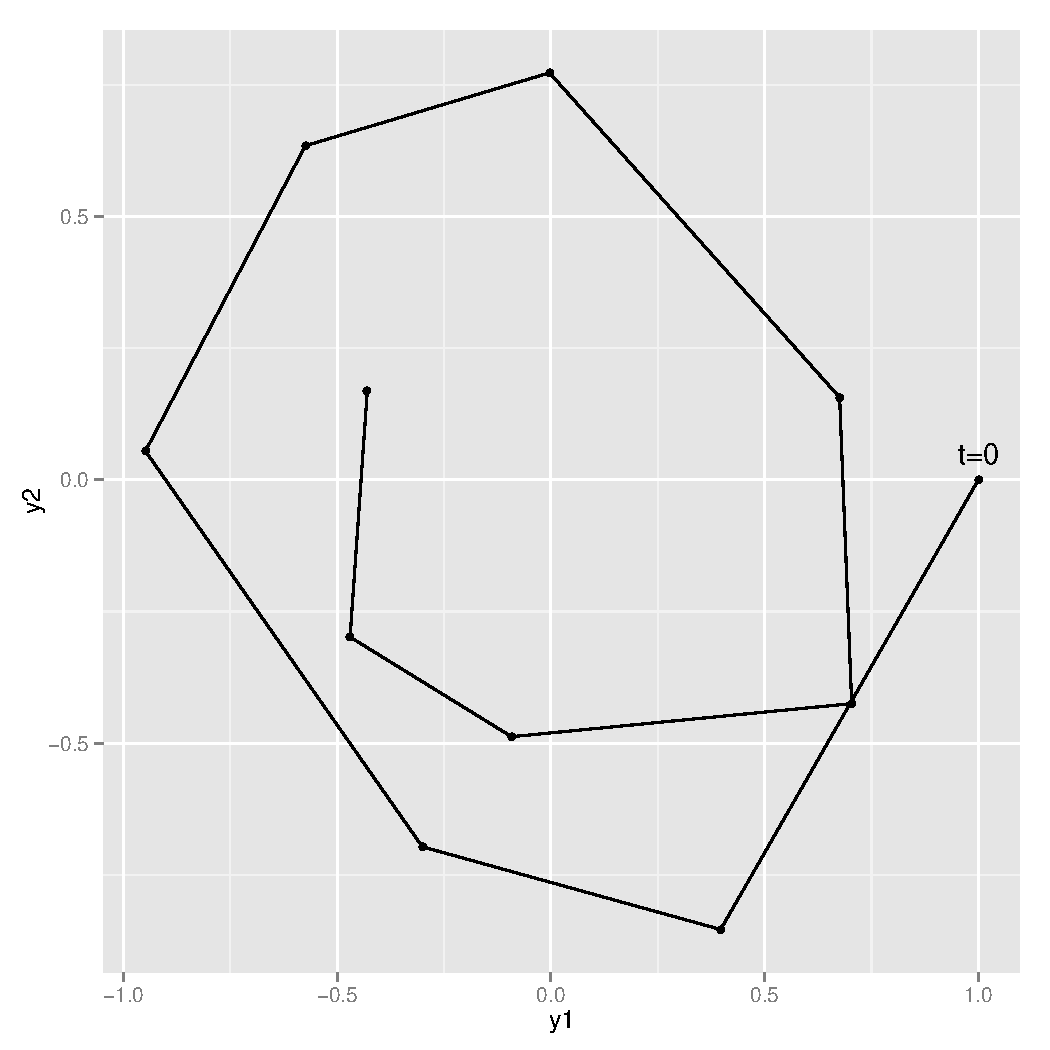
\includegraphics[height=2in]{img/sho-ode-trajectory.pdf}%
\end{center}
\vspace*{-0.25in}
\caption{\small\it Trajectory of the simple harmonic oscillator given
  parameter $\theta=0.15$ and initial condition $y(t=0) = (1,0)$ with
  additional independent\ $\distro{Normal}(0,0.1)$ measurement error
  in both dimensions.}%
\label{sho-trajectory.figure}
\end{figure}



\subsection{Simulating Noisy Measurements}

The data used to make this plot is derived from the Stan model to
simulate noisy observations given in \reffigure{sho-sim}.
%
\begin{figure}
\begin{quote}\small
\begin{Verbatim}
functions {
  real[] sho(real t,
             real[] y, 
             real[] theta,
             real[] x_r,
             int[] x_i) {
    real dydt[2];
    dydt[1] <- y[2];
    dydt[2] <- -y[1] - theta[1] * y[2];
    return dydt;
  }
}
data {
  int<lower=1> T;
  real y0[2];
  real t0;
  real ts[T];
  real theta[1];
}
transformed data {
  real x_r[0];
  int x_i[0];
}
model {
}
generated quantities {
  real y_hat[T,2];
  y_hat <- integrate_ode(sho, y0, t0, ts, theta, x_r, x_i);

  // add measurement error
  for (t in 1:T) {
    y_hat[t,1] <- y_hat[t,1] + normal_rng(0,0.1);
    y_hat[t,2] <- y_hat[t,2] + normal_rng(0,0.1);
  }
}
\end{Verbatim}
\end{quote}
\vspace*{-0.2in}
\caption{\small\it Stan program to simulate noisy measurements from a
  simple harmonic oscillator.  The system of differential equations is
  coded as a function.  The system parameters \code{theta} and initial
  state \code{y0} are read in as data along with the initial time
  \code{t0} and observation times \code{ts}. The generated quantities
  block is used to solve the ODE for the specified times and then add
  random measurement error, producing observations \code{y\_hat}.}\label{sho-sim.figure}
\end{figure}

This program illustrates the way in which the ODE solver is called in
a Stan program,
%
\begin{quote}
\begin{Verbatim}
y_hat <- integrate_ode(sho, y0, t0, ts, theta, x_r, x_i);
\end{Verbatim}
\end{quote}
%
This assigns the solutions to the system defined by function
\code{sho}, given initial state \code{y0}, initial time \code{t0},
requested solution times \code{ts}, parameters \code{theta}, real data
\code{x}, and integer data \code{x\_int}.

Here, the ODE solver is called in the generated quantities block to
provide a $10 \times 2$ array of solutions \code{y\_hat} to
which measurement error is added using the normal pseudo-random number
generating function \code{normal\_rng}.  The number of rows in the
solution array is the same as the size of \code{ts}, the requested
solution times.

\subsection{Estimating System Parameters and Initial State}

Stan provides statistical inference for unknown initial states and/or
parameters.  The ODE solver will be used deterministically to produce
predictions, much like the linear predictor does in a generalized
linear model.  These states will then be observed with measurement error.

%
\begin{figure}
\begin{quote}\small
\begin{Verbatim}
functions {
  real[] sho(real t,
             real[] y, 
             real[] theta,
             real[] x_r,
             int[] x_i) {
    real dydt[2];
    dydt[1] <- y[2];
    dydt[2] <- -y[1] - theta[1] * y[2];
    return dydt;
  }
}
data {
  int<lower=1> T;
  real y[T,2];
  real t0;
  real ts[T];
}
transformed data {
  real x_r[0];
  int x_i[0];
}
parameters {
  real y0[2];
  vector<lower=0>[2] sigma;
  real theta[1];
}
model {
  real y_hat[T,2];
  sigma ~ cauchy(0,2.5);
  theta ~ normal(0,1);
  y0 ~ normal(0,1);
  y_hat <- integrate_ode(sho, y0, t0, ts, theta, x_r, x_i);
  for (t in 1:T)
    y[t] ~ normal(y_hat[t], sigma);
}
\end{Verbatim}
\end{quote}
\vspace*{-0.2in}
\caption{\small\it Stan program to estimate unknown initial conditions
  \code{y0} and system parameter \code{theta} for the simple harmonic
  oscillator with independent normal measurement
  error.}\label{sho-both.figure}
\end{figure}
%
A Stan program that can be used to estimate both the initial state and
parameter value for the simple harmonic oscillator given noisy
observations is given in \reffigure{sho-both}.  Compared to the
simulation model in \reffigure{sho-sim}, the model to estimate
parameters uses the \code{integrate\_ode} function in the model block
rather than the generated quantities block.  There are Cauchy priors on the
measurement error scales \code{sigma} and unit normal priors on the
components of parameter array \code{theta} and initial state parameter
array \code{y0}.  The solutions to the ODE are then assigned to an
array \code{y\_hat}, which is then used as the location in the
observation noise model as follows.
%
\begin{quote}
\begin{Verbatim}
y_hat <- integrate_ode(sho, y0, t0, ts, theta, x_r, x_i);
for (t in 1:T)
  y[t] ~ normal(y_hat[t], sigma);
\end{Verbatim}
\end{quote}
%
As with other regression-like models, it's easy to change the noise
model to be robust (e.g., Student-t distributed), to be correlated in
the state variables (e.g., with a multivariate normal distribution),
or both (e.g., with a multivariate Student-t distribution).

In this simple model with independent noise scales of 0.10, 10
observed data points for times $t = 1, ..., 10$ is sufficient to
reliably estimate the ODE parameter, initial state, and noise scales.



\section{Stiff ODEs}

Stan's approach will not be efficient for stiff systems of ODEs,
roughly characterized as systems presenting numerical difficulties for
gradient-based stepwise solvers.  Stiffness typically arises due to high
curvature in the solution space.%
%
\footnote{Not coincidentally, high curvature in the posterior of a
  general Stan model poses the same kind of problem for Euclidean
  Hamiltonian Monte Carlo (HMC) sampling.  The reason is that HMC is
  based on the leapfrog algorithm, a gradient-based, stepwise
  numerical differential equation solver specialized for Hamiltonian
  systems with separable potential and kinetic energy terms.}
%
It will work, but can be slow enough to be impractical because the
stepwise integrator used for the solutions will have to take very
small steps to ensure adequate solution accuracy.  In the future, we hope to
roll out a more efficient approach to stiff ODEs in which automatic
differentiation can be applied to compute the Jacobian of the final
coupled system of state variables and partials with respect to
parameters.


\chapter{Problematic Posteriors}\label{problematic-posteriors.chapter}%
\noindent
Mathematically speaking, with a proper posterior, one can do Bayesian
inference and that's that. There is not even a need to require a
finite variance or even a finite mean---all that's needed is a finite
integral.  Nevertheless, modeling is a tricky business and even
experienced modelers sometimes code models that lead to improper
priors.  Furthermore, some posteriors are mathematically sound, but
ill-behaved in practice.  This chapter discusses issues in models that
create problematic posterior inferences, either in general for
Bayesian inference or in practice for Stan.


\section{Collinearity of Predictors in Regressions}\label{collinearity.section}

This section discusses problems related to the classical notion of
identifiability, which lead to ridges in the posterior density and
wreak havoc with both sampling and inference.

\subsection{Examples of Collinearity}

\subsubsection{Redundant Intercepts}

The first example of collinearity is an artificial example involving
redundant intercept parameters.%
%
\footnote{This example was raised by Richard McElreath on the Stan
  users group in a query about the difference in behavior between
  Gibbs sampling as used in BUGS and JAGS and the Hamiltonian Monte
  Carlo (HMC) and no-U-turn samplers (NUTS) used by Stan.}
%
Suppose there are observations $y_n$ for $n \in 1{:}N$, 
two intercept parameters $\lambda_1$ and
$\lambda_2$, a scale parameter $\sigma > 0$, and the sampling distribution
%
\[
y_n \sim \distro{Normal}(\lambda_1 + \lambda_2, \sigma).
\]
%
For any constant $q$, the sampling density for $y$ does not change if
we add $q$ to $\lambda_1$ and subtract it from $\lambda_2$, i.e.,
%
\[
p(y | \lambda_1, \lambda_2,\sigma)
=
p(y | \lambda_1 + q, \lambda_2 - q, \sigma).
\]
%
The consequence is that an improper uniform prior $p(\mu,\sigma)
\propto 1$ leads to an improper posterior.  This impropriety arises
because the neighborhoods around $\lambda_1 + q, \lambda_1 - q$ have
the same mass no matter what $q$ is.  Therefore, a sampler would need
to spend as much time in the neighborhood of $\lambda_1=1000000000$
and $\lambda_2=-1000000000$ as it does in the neighborhood of
$\lambda_1=0$ and $\lambda_2=0$, and so on for ever more far-ranging
values.

The maringal posterior $p(\lambda_1,\lambda_2|y)$ for this model is
thus improper.%
%
\footnote{The marginal posterior $p(\sigma|y)$ for $\sigma$ is proper
  here as long as there are at least two distinct data points.}
%
The impropriety shows up visually as a ridge in the posterior density,
as illustrated in the left-hand figure of
\reffigure{non-identifiable-density}.  The ridge for this model is
along the line where $\lambda_2 = \lambda_1 + c$ for some constant
$c$.  

Contrast this model with a simple regression with a single intercept
parameter $\mu$ and sampling distribution
\[
y_n \sim \distro{Normal}(\mu,\sigma).
\]
Even with an improper prior, the posterior is proper as long as there
are at least two data points $y_n$ with distinct values.


\subsubsection{Ability and Difficulty in IRT Models}

Consider an item-response theory model for students $j \in 1{:}J$ with
abilities $\alpha_j$ and test items $i \in 1{:}I$ with difficulties
$\beta_i$.  The observed data is an $I \times J$ array with entries
$y_{i,j} \in \{ 0, 1 \}$ coded such that $y_{i,j} = 1$ indicates that
student $j$ answered question $i$ correctly.  The sampling
distribution for the data is
%
\[
y_{i,j} \sim \distro{Bernoulli}(\mbox{logit}^{-1}(\alpha_j - \beta_i)).
\]
%
For any constant $c$, the probability of $y$ is unchanged by adding a
constant $c$ to all the abilities and subtracting it from all the
difficulties, i.e.,
%
\[
p(y | \alpha, \beta)
= 
p(y | \alpha + c, \beta - c).
\]
%
This leads to a multivariate version of the ridge displayed by the
regression with two intercepts discussed above.

\subsubsection{General Collinear Regression Predictors}

The general form of the collinearity problem arises when predictors
for a regression are collinear.  For example, consider a linear
regression sampling distribution
\[
y_n \sim \distro{Normal}(x_n \beta, \sigma)
\]
for an $N$-dimensional observation vector $y$, an $N \times K$ predictor
matrix $x$, and a $K$-dimensional coefficient vector $\beta$.

Now suppose that column $k$ of the predictor matrix is a multiple of
column $k'$, i.e., there is some constant $c$ such that $x_{n,k} = c
\, x_{n,k'}$ for all $n$.  In this case, the coefficients $\beta_k$
and $\beta_{k'}$ can covary without changing the predictions, so that
for any $d \neq 0$,
%
\[
p(y | \ldots, \beta_k, \ldots, \beta_{k'}, \ldots, \sigma)
=
p(y | \ldots, d  \beta_k, \ldots, \frac{d}{c} \, \beta_{k'}, \ldots,
\sigma).
\]

Even if columns of the predictor matrix are not exactly collinear as
discussed above, they cause similar problems for inference if they are
nearly collinear.


\subsubsection{Multiplicative Issues with Discrimination in IRT}

Consider adding a discrimination parameter $\delta_i$ for each
question in an IRT model, with data sampling model
\[
y_{i,j} \sim \distro{Bernoulli}(\mbox{logit}^{-1}(\delta_i(\alpha_j - \beta_i))).
\]
For any constant $c \neq 0$, multiplying $\delta$ by $c$ and dividing
$\alpha$ and $\beta$ by $c$ produces the same likelihood,
\[
p(y|\delta,\alpha,\beta)
= p(y|c \delta, \, \frac{1}{c}\alpha, \, \frac{1}{c}\beta).
\]
If $c < 0$, this switches the signs of every component in $\alpha$,
$\beta$, and $\delta$ without changing the density.


\subsubsection{Softmax with $K$ vs. $K-1$ Parameters}

In order to parameterize a $K$-simplex (i.e., a $K$-vector with
non-negative values that sum to one), only $K - 1$ parameters are
necessary because the $K$th is just one minus the sum of the first $K
- 1$ parameters, so that if $\theta$ is a $K$-simplex,
%
\[
\theta_K = 1 - \sum_{k=1}^K \theta_k.
\]
%
The softmax function (see \refsection{softmax}) maps a $K$-vector
$\alpha$ of linear predictors to a $K$-simplex $\theta =
\mbox{softmax}(\alpha)$ by defining
%
\[
\theta_k = \frac{\exp(\alpha_k)}{\sum_{k'=1}^K \exp(\alpha_k')}.
\]
%
The softmax function is many-to-one, which leads to a lack of
identifiability of the unconstrained parameters $\alpha$.  In
particular, adding or subtracting a constant from each $\alpha_k$
produces the same simplex $\theta$. 



\subsection{Mitigating the Invariances}

All of the examples discussed in the previous section allow
translation or scaling of parameters while leaving the data
probability density invariant.  These problems can be mitigated in
several ways.

\subsubsection{Removing Redundant Parameters or Predictors}

In the case of the multiple intercepts, $\lambda_1$ and $\lambda_2$,
the simplest solution is to remove the redundant intercept, resulting
in a model with a single intercept parameter $\mu$ and sampling
distribution $y_n \sim \distro{Normal}(\mu, \sigma)$.  The same
solution works for solving the problem with collinearity---just remove
one of the columns of the predictor matrix $x$.

\subsubsection{Pinning Parameters}

The IRT model without a discrimination parameter can be fixed by
pinning one of its parameters to a fixed value, typically 0.  For
example, the first student ability $\alpha_1$ can be fixed to 0.  Now
all other student ability parameters can be interpreted as being
relative to student 1.  Similarly, the difficulty parameters are
interpretable relative to student 1's ability to answer them.

This solution is not sufficient to deal with the multiplicative
invariance introduced by the question discrimination parameters
$\delta_i$.  To solve this problem, one of the difficulty parameters,
say $\delta_1$, must also be constrained.  Because it's a
multiplicative and not an additive invariance, it must be constrained
to a non-zero value, with 1 being a convenient choice.  Now all of the
discrimination parameters may be interpreted relative to item 1's
discrimination.

The many-to-one nature of $\mbox{softmax}(\alpha)$ is typically
mitigated by pinning a component of $\alpha$, for instance fixing
$\alpha_K = 0$.  The resulting mapping is one-to-one from $K-1$
unconstrained parameters to a $K$-simplex.  This is roughly how
simplex-constrained parameters are defined in Stan; see
\refsection{simplex-transform} for a precise definition.  The Stan
code for creating a simplex from a $K-1$-vector can be written as
%
\begin{quote}
\begin{Verbatim}
vector softmax_id(vector alpha) {
  vector[num_elements(alpha) + 1] alphac1;
  for (k in 1:num_elements(alpha))
    alphac1[k] <- alpha[k];
  alpha[num_elements(alphac)] <- 0;
  return softmax(alphac);
}
\end{Verbatim}
\end{quote}




\subsubsection{Adding Priors}

So far, the models have been discussed as if the priors on the
parameters were improper uniform priors.  

A more general Bayesian solution to these invariance problems is to
impose proper priors on the parameters.  This approach can be used to
solve problems arising from either additive or multiplicative
invariance.

For example, normal priors on the multiple intercepts,
\[
\lambda_1, \lambda_2 \sim \distro{Normal}(0,\tau),
\]
with a constant scale $\tau$, ensure that the posterior mode is
located at a point where $\lambda_1 = \lambda_2$, because this
minimizes $\log \distro{Normal}(\lambda_1|0,\tau) + \log
\distro{Normal}(\lambda_2|0,\tau)$.%
%
\footnote{A Laplace prior (or an L1 regularizer for penalized maximum
  likelihood estimation) is not sufficient to remove this additive
  invariance.  It provides shrinkage, but does not in and of itself
  identify the parameters because adding a constant to $\lambda_1$ and
  subtracting it from $\lambda_2$ results in the same value for the
  prior density.}
%
\begin{figure}
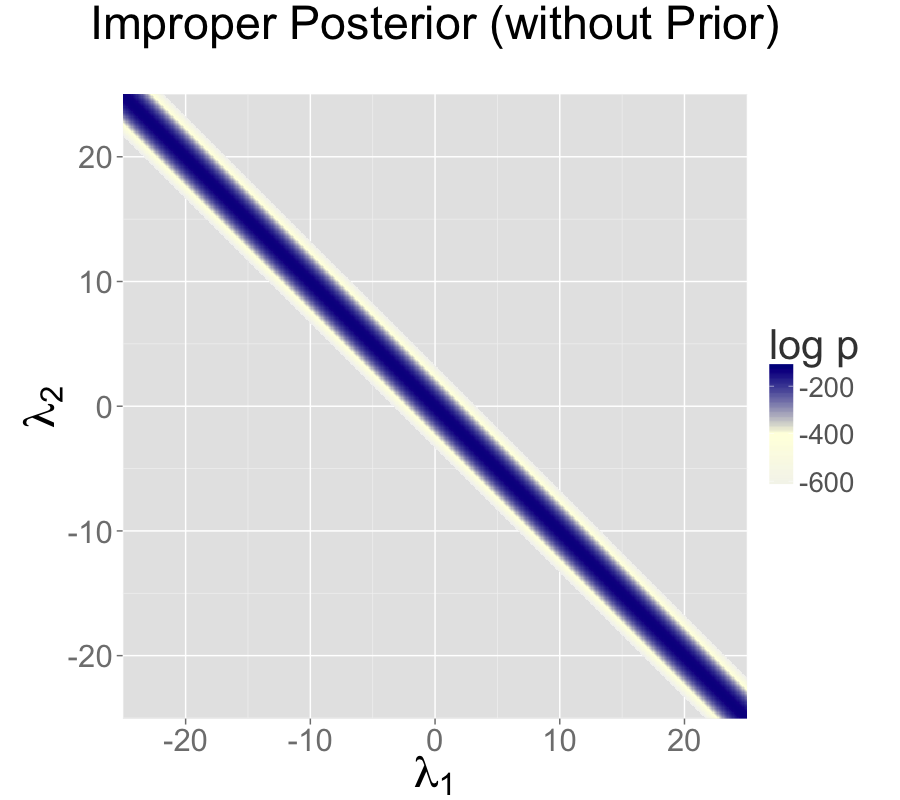
\includegraphics[height=1.45in]{img/non-identified.png}%
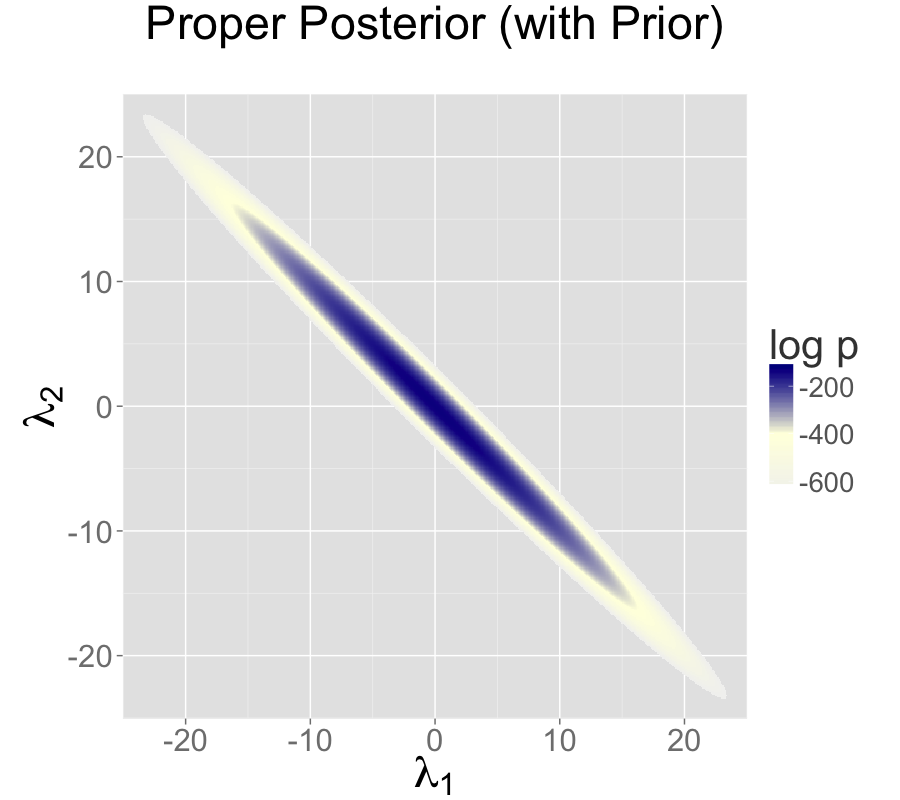
\includegraphics[height=1.45in]{img/non-identified-plus-prior.png}%
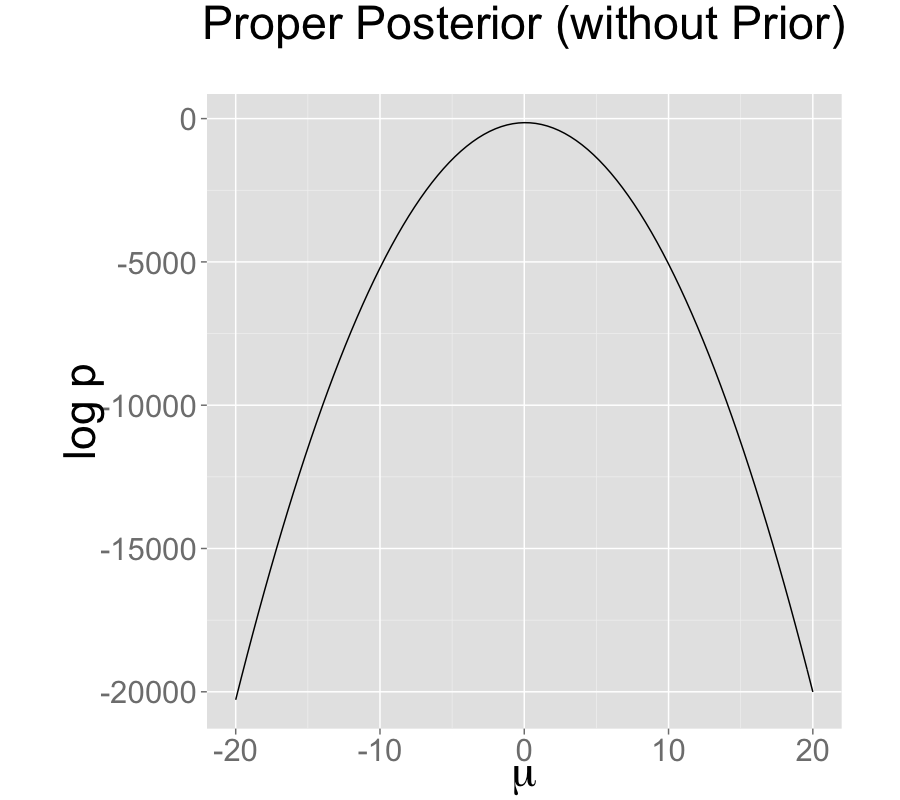
\includegraphics[height=1.45in]{img/one-param-identified.png}
\vspace*{-.1in}
\caption{\small\it Posteriors for two intercept parameterization
  without prior, two intercept parameterization with unit normal
  prior, and one intercept reparameterization without prior.  For all
  three cases, the posterior is plotted for 100 data points drawn from
  a unit normal. Left) The two intercept parameterization leads to an
  improper prior with a ridge extending infinitely to the northwest
  and southeast.  Middle) Adding a unit normal prior for the
  intercepts results in a proper posterior.  Right) The single
  intercept parameterization with no prior also has a proper posterior.}%
\label{non-identifiable-density.figure}
\end{figure}
%
The addition of a prior to the two intercepts model is shown in the
middle plot in \reffigure{non-identifiable-density}.  The plot on
the right of \reffigure{non-identifiable-density} shows the result of
reparameterizing to a single intercept.

An alternative strategy for identifying a $K$-simplex parameterization
$\theta = \mbox{softmax}(\alpha)$ in terms of an unconstrained
$K$-vector $\alpha$ is to place a prior on the components of $\alpha$
with a fixed location (that is, specifically avoid hierarchical priors
with varying location).  Unlike the approaching of pinning $\alpha_K =
0$, the prior-based approach models the $K$ outcomes symmetrically
rather than modeling $K-1$ outcomes relative to the $K$-th.  The
pinned parameterization, on the other hand, is usually more efficient
statisticaly because it does not have the extra degree of (prior
constrained) wiggle room.


\subsubsection{Vague, Strongly Informative, and Weakly Informative Priors}

Care must be used when adding a prior to resolve invariances.  If the
prior is taken to be too broad (i.e., too vague), the resolution is in
theory only, and samplers will still struggle.  

Ideally, a realistic prior will be formulated based on substantive
knowledge of the problem being modeled.  Such a prior can be chosen to
have the appropriate strength based on prior knowledge.  A strongly
informative prior makes sense if there is strong prior information.

When there is not strong prior information, a weakly informative prior
strikes the proper balance between controlling computational inference
without dominating the data in the posterior.  In most problems, the
modeler will have at least some notion of the expected scale of the
estimates and be able to choose a prior for identification purposes
that does not dominate the data, but provides sufficient computational
control on the posterior.

Priors can also be used in the same way to control the additive
invariance of the IRT model.  A typical approach is to place a strong
prior on student ability parameters $\alpha$ to control scale simply
to control the additive invariance of the basic IRT model and the
multiplicative invariance of the model extended with a item
discrimination parameters; such a prior does not add any prior
knowledge to the problem.  Then a prior on item difficulty can be
chosen that is either informative or weakly informative based on prior
knowledge of the problem.


\section{Label Switching in Mixture Models}\label{label-switching-problematic.section}

Where collinearity in regression models can lead to infinitely many
posterior maxima, swapping components in a mixture model leads to
finitely many posterior maxima.

\subsection{Mixture Models}

Consider a normal mixture model with two location parameters $\mu_1$
and $\mu_2$, a shared scale $\sigma > 0$, a mixture ratio $\theta \in
[0,1]$, and likelihood
\[
p(y|\theta,\mu_1,\mu_2,\sigma) 
= \prod_{n=1}^N \big( \theta \, \distro{Normal}(y_n|\mu_1,\sigma)
                       + (1 - \theta) \, \distro{Normal}(y_n|\mu_2,\sigma) \big).
\]
The issue here is exchangeability of the mixture components, because
\[
p(\theta,\mu_1,\mu_2,\sigma|y) = p((1-\theta),\mu_2,\mu_1,\sigma|y).
\]
The problem is exacerbated as the number of mixture components $K$
grows, as in clustering models, leading to $K!$ identical posterior
maxima.

\subsection{Convergence Monitoring and Effective Sample Size}

The analysis of posterior convergence and effective sample size is
also difficult for mixture models.  For example, the $\hat{R}$
convergence statistic reported by Stan and the computation of
effective sample size are both compromised by label switching.  The
problem is that the posterior mean, a key ingredient in these
computations, is affected by label switching, resulting in a posterior
mean for $\mu_1$ that is equal to that of $\mu_2$, and a posterior
mean for $\theta$ that is always 1/2, no matter what the data is. 

\subsection{Some Inferences are Invariant}

In some sense, the index (or label) of a mixture component is
irrelevant.  Posterior predictive inferences can still be carried out
without identifying mixture components.  For example, the log
probability of a new observation does not depend on the identities of
the mixture components.  The only sound Bayesian inferences in such
models are those that are invariant to label switching.  Posterior
means for the parameters are meaningless because they are not
invariant to label switching; for example, the posterior mean for
$\theta$ in the two component mixture model will always be 1/2.

\subsection{Highly Multimodal Posteriors}

Theoretically, this should not present a problem for inference because
all of the integrals involved in posterior predictive inference will
be well behaved. The problem in practice is computation. 

Being able to carry out such invariant inferences in practice is an
altogether different matter.  It is almost always intractable to find
even a single posterior mode, much less balance the exploration of the
neighborhoods of multiple local maxima according to the probability
masses. In Gibbs sampling, it is unlikely for $\mu_1$
to move to a new mode when sampled conditioned on the current values
of $\mu_2$ and $\theta$. For HMC and NUTS, the problem is that the
sampler gets stuck in one of the two ``bowls'' arounds the modes and
cannot gather enough energy from random momentum assignment to move
from one mode to another.

Even with a proper posterior, all known sampling and inference
techniques are notoriously ineffective when the number of modes grows
super-exponentially as it does for mixture models with increasing
numbers of components.

\subsection{Hacks as Fixes}

Several hacks (i.e., ``tricks'') have been suggested and employed to
deal with the problems posed by label switching in practice.

\subsubsection{Parameter Ordering Constraints}

One common strategy is to impose a constraint on the parameters that
identifies the components.  For instance, we might consider
constraining $\mu_1 < \mu_2$ in the two-component normal mixture model
discussed above.  A problem that can arise from such an approach is
when there is substantial probabilty mass for the opposite ordering
$\mu_1 > \mu_2$.  In these cases, the the posteriors are affected by
the constraint and true posterior uncertainty in $\mu_1$ and $\mu_2$
is not captured by the model with the constraint.  In addition,
standard approaches to posterior inference for event probabilities is
compromised.  For instance, attempting to use $M$ posterior samples to
estimate $\mbox{Pr}[\mu_1 > \mu_2]$, will fail, because the estimator
\[
\mbox{Pr}[\mu_1 > \mu_2] 
\approx 
\sum_{m=1}^M \mbox{I}(\mu_1^{(m)} > \mu_2^{(m)})
\]
will result in an estimate of 0 because the posterior respects the
constraint in the model.  

\subsubsection{Initialization around a Single Mode}

Another common approach is to run a single chain or to initialize the
parameters near realistic values.%
%
\footnote{Tempering methods may be viewed as automated ways to carry
  out such a search for modes, though most MCMC tempering methods
  continue to search for modes on an ongoing basis; see
  \citep{SwendsenWang:1986, Neal:1996b}.}
%
This can work better than the hard constraint approach if reasonable
initial values can be found and the labels do not switch within a
Markov chain.  The result is that all chains are glued to a
neighborhood of a particular mode in the posterior.



\section{Posteriors with Unbounded Densities}

In some cases, the posterior density grows without bounds as
parameters approach certain poles or boundaries.  In such, there
are no posterior modes and numerical stability issues can arise as
sampled parameters approach constraint boundaries.

\subsection{Mixture Models with Varying Scales}

One such example is a binary mixture model with scales varying by
component, $\sigma_1$ and $\sigma_2$ for locations $\mu_1$ and
$\mu_2$. In this situation, the density grows without bound as
$\sigma_1 \rightarrow 0$ and $\mu_1 \rightarrow y_n$ for some $n$;
that is, one of the mixture components concentrates all of its mass
around a single data item $y_n$.

\subsection{Beta-Binomial Models with Skewed Data and Weak Priors}

Another example of unbounded densities arises with a posterior such as
$\distro{Beta}(\phi|0.5,0.5)$, which can arise if very ``weak'' beta
priors are used for groups that have no data. This density is
unbounded as $\phi \rightarrow 0$ and $\phi \rightarrow 1$. Similarly,
a Bernoulli likelihood model coupled with a ``weak'' beta prior, leads
to a posterior
%
\begin{eqnarray*}
p(\phi|y) 
& \propto & \textstyle
\distro{Beta}(\phi|0.5,0.5) \times \prod_{n=1}^N \distro{Bernoulli}(y_n|\phi)
\\[4pt]
& = &\textstyle
\distro{Beta}(\phi \, | \, 0.5 + \sum_{n=1}^N y_n, \ \ 0.5 + N - \sum_{n=1}^N y_n).
\end{eqnarray*}
%
If $N = 9$ and each $y_n = 1$, the posterior is
$\distro{Beta}(\phi|9.5,0,5)$.  This posterior is unbounded as $\phi
\rightarrow 1$.  Nevertheless, the posterior is proper, and although
there is no posterior mode, the posterior mean is well-defined with a
value of exactly 0.95.

\subsubsection{Constrained vs.\ Unconstrained Scales}

Stan does not sample directly on the constrained $(0,1)$ space for
this problem, so it doesn't directly deal with unconstrained density
values.  Rather, the probability values $\phi$ are logit-transformed
to $(-\infty,\infty)$.  The boundaries at 0 and 1 are pushed out to
$-\infty$ and $\infty$ respectively.  The Jacobian adjustment that
Stan automatically applies ensures the unconstrained density is
proper.  The adjustment for the particular case of $(0,1)$ is $\log
\mbox{logit}^{-1}(\phi) + \log \mbox{logit}(1 - \phi)$; see
\refsection{logit-transform-jacobian} for the derivation.

There are two problems that still arise, though.  The first is that if
the posterior mass for $\phi$ is near one of the boundaries, the
logit-transformed parameter will have to sweep out very long paths and
thus can dominate the U-turn condition imposed by the no-U-turn
sampler (NUTS).  The second issue is that the inverse transform from
the unconstrained space to the constrained space can underflow to 0 or
overflow to 1, even when the unconstrained parameter is not infinite.
Similar problems arise for the expectation terms in logistic
regression, which is why the logit-scale parameterizations of the
Bernoulli and binomial distributions are more stable.



\section{Posteriors with Unbounded Parameters}

In some cases, the posterior density will not grow without bound, but
parameters will grow without bound with gradually increasing density
values.  Like the models discussed in the previous section that have
densities that grow without bound, such models also have no posterior
modes.


\subsection{Separability in Logistic Regression}

Consider a logistic regression model with $N$ observed outcomes $y_n
\in \{ 0, 1 \}$, an $N \times K$ matrix $x$ of predictors, a
$K$-dimensional coefficient vector $\beta$, and sampling distribution
\[
y_n \sim \distro{Bernoulli}(\mbox{logit}^{-1}(x_n \beta)).
\]
Now suppose that column $k$ of the predictor matrix is such that
$x_{n,k} > 0$ if and only if $y_n = 1$, a condition known as
``separability.''  In this case, predictive accuracy on the observed data
continue to improve as $\beta_k \rightarrow \infty$, because for cases
with $y_n = 1$, $x_n \beta \rightarrow \infty$ and hence
$\mbox{logit}^{-1}(x_n \beta) \rightarrow 1$.  

With separability, there is no maximum to the likelihood and hence no
maximum likelihood estimate.  From the Bayesian perspective, the
posterior is improper and therefor the marginal posterior mean for
$\beta_k$ is also not defined.  The usual solution to this problem in
Bayesian models is to include a proper prior for $\beta$, which
ensures a proper posterior.


\section{Uniform Posteriors}

Suppose your model includes a parameter $\psi$ that is defined on
$[0,1]$ and is given a flat prior $\distro{Uniform}(\psi|0,1)$. Now if
the data don't tell us anything about $\psi$, the posterior is also
$\distro{Uniform}(\psi|0,1)$.

Although there is no maximum likelihood estimate for $\psi$, the
posterior is uniform over a closed interval and hence proper.  In the
case of a uniform posterior on $[0,1]$, the posterior mean for $\psi$
is well-defined with value $1/2$.  Although there is no posterior
mode, posterior predictive inference may nevertheless do the right
thing by simply integrating (i.e., averaging) over the predictions for
$\psi$ at all points in $[0,1]$.


\section{Sampling Difficulties with Problematic Priors}

With an improper posterior, it is theoretically impossible to properly
explore the posterior. However, Gibbs sampling as performed by BUGS
and JAGS, although still ineable to properly sample from such an
improper posterior, behaves quite differently in practice than the
Hamiltonian Monte Carlo sampling performed by Stan when faced with an
example such as the two intercept model discussed in
\refsection{collinearity} and illustrated in
\reffigure{non-identifiable-density}.

\subsection{Gibbs Sampling}

Gibbs sampling, as performed by BUGS and JAGS, may appear to be
efficient and well behaved for this unidentified model, but as
discussed in the previous subsection, will not actually explore the
posterior properly.

Consider what happens with initial values $\lambda_1^{(0)}, \lambda_2^{(0)}$.
Gibbs sampling proceeds in iteration $m$ by drawing
%
\begin{eqnarray*}
\lambda_1^{(m)} 
& \sim & p(\lambda_1 \, | \, \lambda_2^{(m-1)}, \, \sigma^{(m-1)}, \, y)
\\[6pt]
\lambda_2^{(m)}
& \sim & p(\lambda_2 \, | \, \lambda_1^{(m)}, \, \sigma^{(m-1)}, \, y)
\\[6pt]
\sigma^{(m)} 
& \sim & p(\sigma \, | \, \lambda_1^{(m)}, \, \lambda_2^{(m)}, \, y).
\end{eqnarray*}
%
Now consider the draw for $\lambda_1$ (the draw for $\lambda_2$ is
symmetric), which is conjugate in this model and thus can be done very
efficiently.  In this model, the range from which the next $\lambda_1$
can be drawn is highly constrained by the current values of
$\lambda_2$ and $\sigma$.  Gibbs will run very quickly and provide
seemingly reasonable inferences for $\lambda_1 + \lambda_2$.  But it
will not explore the full range of the posterior; it will merely take
a slow random walk from the initial values.  This random walk behavior
is typical of Gibbs sampling when posteriors are highly correlated and
the primary reason to prefer Hamiltonian Monte Carlo to Gibbs sampling
for models with parameters correlated in the posterior.

\subsection{Hamiltonian Monte Carlo Sampling}

Hamiltonian Monte Carlo (HMC), as performed by Stan, is much more
efficient at exploring posteriors in models where parameters are
correlated in the posterior.  In this particular example, the
Hamiltonian dynamics (i.e., the motion of a fictitious particle given
random momentum in the field defined by the negative log posterior) is
going to run up and down along the valley defined by the potential
energy (ridges in log posteriors correspond to valleys in potential
energy).  In practice, even with a random momentum for $\lambda_1$ and
$\lambda_2$, the gradient of the log posterior is going to adjust for
the correlation and the simulation will run $\lambda_1$ and
$\lambda_2$ in opposite directions along the valley corresponding to
the ridge in the posterior log density (see
\reffigure{non-identifiable-density}.  

\subsection{No-U-Turn Sampling}

Stan's default no-U-turn sampler (NUTS), is even more efficient at
exploring the posterior (see
\citep{Hoffman-Gelman:2011,Hoffman-Gelman:2014}).  NUTS simulates the
motion of the fictitious particle representing the parameter values
until it makes a U-turn, it will be defeated in most cases, as it will
just move down the potential energy valley indefinitely without making
a U-turn. What happens in practice is that the maximum number of
leapfrog steps in the simulation will be hit in many of the
iterations, causing a very large number of log probability and
gradient evaluations (1000 if the max tree depth is set to 10, as in
the default). Thus sampling will appear to be very slow.  This is
indicative of an improper posterior, not a bug in the NUTS algorithm
or its implementation.  It is simply not possible to sample from an
improper posterior!  Thus the behavior of HMC in general and NUTS
in particular should be reassuring in that it will clearly fail in
cases of improper posteriors, resulting in a clean diagnostic of
sweeping out very large paths in the posterior.  

\begin{figure}
%
\normalsize {\it Two Scale Parameters, Improper Prior}
%
\footnotesize
\begin{Verbatim}
Inference for Stan model: improper_stan
Warmup took (2.7, 2.6, 2.9, 2.9) seconds, 11 seconds total
Sampling took (3.4, 3.7, 3.6, 3.4) seconds, 14 seconds total

                  Mean     MCSE   StdDev        5%       95%  N_Eff  N_Eff/s  R_hat
lp__          -5.3e+01  7.0e-02  8.5e-01  -5.5e+01  -5.3e+01    150       11    1.0
n_leapfrog__   1.4e+03  1.7e+01  9.2e+02   3.0e+00   2.0e+03   2987      212    1.0
lambda1        1.3e+03  1.9e+03  2.7e+03  -2.3e+03   6.0e+03    2.1     0.15    5.2
lambda2       -1.3e+03  1.9e+03  2.7e+03  -6.0e+03   2.3e+03    2.1     0.15    5.2
sigma          1.0e+00  8.5e-03  6.2e-02   9.5e-01   1.2e+00     54      3.9    1.1
mu             1.6e-01  1.9e-03  1.0e-01  -8.3e-03   3.3e-01   2966      211    1.0
\end{Verbatim}
%
\vspace*{12pt}
%
\normalsize
{\it Two Scale Parameters, Weak Prior}
%
\footnotesize
\begin{Verbatim}
Warmup took (0.40, 0.44, 0.40, 0.36) seconds, 1.6 seconds total
Sampling took (0.47, 0.40, 0.47, 0.39) seconds, 1.7 seconds total

                 Mean     MCSE   StdDev        5%    95%  N_Eff  N_Eff/s  R_hat
lp__              -54  4.9e-02  1.3e+00  -5.7e+01    -53    728      421    1.0
n_leapfrog__      157  2.8e+00  1.5e+02   3.0e+00    511   3085     1784    1.0
lambda1          0.31  2.8e-01  7.1e+00  -1.2e+01     12    638      369    1.0
lambda2         -0.14  2.8e-01  7.1e+00  -1.2e+01     12    638      369    1.0
sigma             1.0  2.6e-03  8.0e-02   9.2e-01    1.2    939      543    1.0
mu               0.16  1.8e-03  1.0e-01  -8.1e-03   0.33   3289     1902    1.0
\end{Verbatim}
%
\vspace*{12pt}
%
\normalsize {\it One Scale Parameter, Improper Prior}
%
\footnotesize
\begin{Verbatim}
Warmup took (0.011, 0.012, 0.011, 0.011) seconds, 0.044 seconds total
Sampling took (0.017, 0.020, 0.020, 0.019) seconds, 0.077 seconds total

                Mean     MCSE  StdDev        5%   50%   95%  N_Eff  N_Eff/s  R_hat
lp__             -54  2.5e-02    0.91  -5.5e+01   -53   -53   1318    17198    1.0
n_leapfrog__     3.2  2.7e-01     1.7   1.0e+00   3.0   7.0     39      507    1.0
mu              0.17  2.1e-03    0.10  -3.8e-03  0.17  0.33   2408    31417    1.0
sigma            1.0  1.6e-03   0.071   9.3e-01   1.0   1.2   2094    27321    1.0
\end{Verbatim}
%
\caption{\small\it Results of Stan runs with default parameters fit to
  $N=100$ data points generated from $y_n \sim \distro{Normal}(0,1)$.
  %
  On the top is the non-identified model with improper uniform priors
  and likelihood $y_n \sim \distro{Normal}(\lambda_1 + \lambda_2,
  \sigma)$. 
  %
  In the middle is the same likelihood as the middle plus priors
  $\lambda_k \sim \distro{Normal}(0,10)$. 
  %
  On the bottom is an identified model with an improper prior, with
  likelihood  $y_n \sim \distro{Normal}(\mu,\sigma)$.  All models
  estimate $\mu$ at roughly 0.16 with very little Monte Carlo standard
  error, but a high posterior standard deviation of 0.1;  the true
  value $\mu=0$ is within the 90\% posterior intervals in all three models.
  %
}%
\label{non-identified-stan-fits.figure}
\end{figure}
%

\subsection{Examples: Fits in Stan}

To illustrate the issues with sampling from non-identified and only
weakly identified models, we fit three models with increasing degrees
of identification of their parameters.  The posteriors for these
models is illustrated in \reffigure{non-identifiable-density}.  The
first model is the unidentified model with two location parameters and
no priors discussed in \refsection{collinearity}.
%
\begin{quote}
\begin{Verbatim}
data {
  int N;
  real y[N];
}
parameters {
  real lambda1;
  real lambda2;
  real<lower=0> sigma;
}
transformed parameters {
  real mu;
  mu <- lambda1 + lambda2;
}
model {
  y ~ normal(mu, sigma);
}
\end{Verbatim}
\end{quote}
%
The second adds priors to the model block for \code{lambda1} and
\code{lambda2} to the previous model.
%
\begin{quote}
\begin{Verbatim}
  lambda1 ~ normal(0,10);
  lambda2 ~ normal(0,10);
\end{Verbatim}
\end{quote}
%
The third involves a single location parameter, but no priors.
%
\begin{quote}
\begin{Verbatim}
data {
  int N;
  real y[N];
}
parameters {
  real mu;
  real<lower=0> sigma;
}
model {
  y ~ normal(mu, sigma);
}
\end{Verbatim}
\end{quote}
%
All three of the example models were fit in Stan 2.1.0 with default
parameters (1000 warmup iterations, 1000 sampling iterations, NUTS
sampler with max tree depth of 10). The results are shown in
\reffigure{non-identified-stan-fits}. The key statistics from these
outputs are the following.
%
\begin{itemize}
\item As indicated by \code{R\_hat} column, all parameters have
  converged other than $\lambda_1$ and $\lambda_2$ in the
  non-identified model.
\item
  The average number of leapfrog steps is roughly 3 in
  the identified model, 150 in the model identified by a weak prior, and
  1400 in the non-identified model.
\item 
  The number of effective samples per
  second for $\mu$ is roughly 31,000 in the identified model, 1900 in the model
  identified with weakly informative priors, and 200 in the
  non-identified model; the results are similar for $\sigma$.  
\item 
  In the non-identified model, the 95\% interval for $\lambda_1$ is
  (-2300,6000), whereas it is only (-12,12) in the model identified with
  weakly informative priors.
\item
  In all three models, the simulated value of $\mu=0$ and $\sigma=1$
  are well within the posterior 90\% intervals.
\end{itemize}
%
The first two points, lack of convergence and hitting the maximum
number of leapfrog steps (equivalently maximum tree depth) are
indicative of improper posteriors.  Thus rather than covering up the
problem with poor sampling as may be done with Gibbs samplers,
Hamiltonian Monte Carlo tries to explore the posterior and its failure
is a clear indication that something is amiss in the model.





\chapter{Optimizing \Stan Code}\label{optimization.chapter}
\noindent
This chapter provides a grab bag of techniques for optimizing \Stan
code, including vectorization, sufficient statistics, and conjugacy.

\section{Reparameterization}\label{reparameterization.section}

Stan's sampler can be slow in sampling from distributions with
difficult posterior geometries.  One way to speed up such models is
through reparameterization.  

\subsection{Example: Neal's Funnel}

In this section, we discuss a general transform from a centered to a
non-centered parameterization \cite{papa-et-al:2007}.%
%
\footnote{This parameterization came to be known on our mailing lists
  as the ``Matt trick'' after Matt Hoffman, who independently came up
  with it while fitting hierarchical models in Stan.}
%
This reparameterization is helpful because it separates the
hierarchical parameters and lower-level parameters in the prior.
%
\begin{figure}[t]
\vspace*{-6pt}
\begin{center}
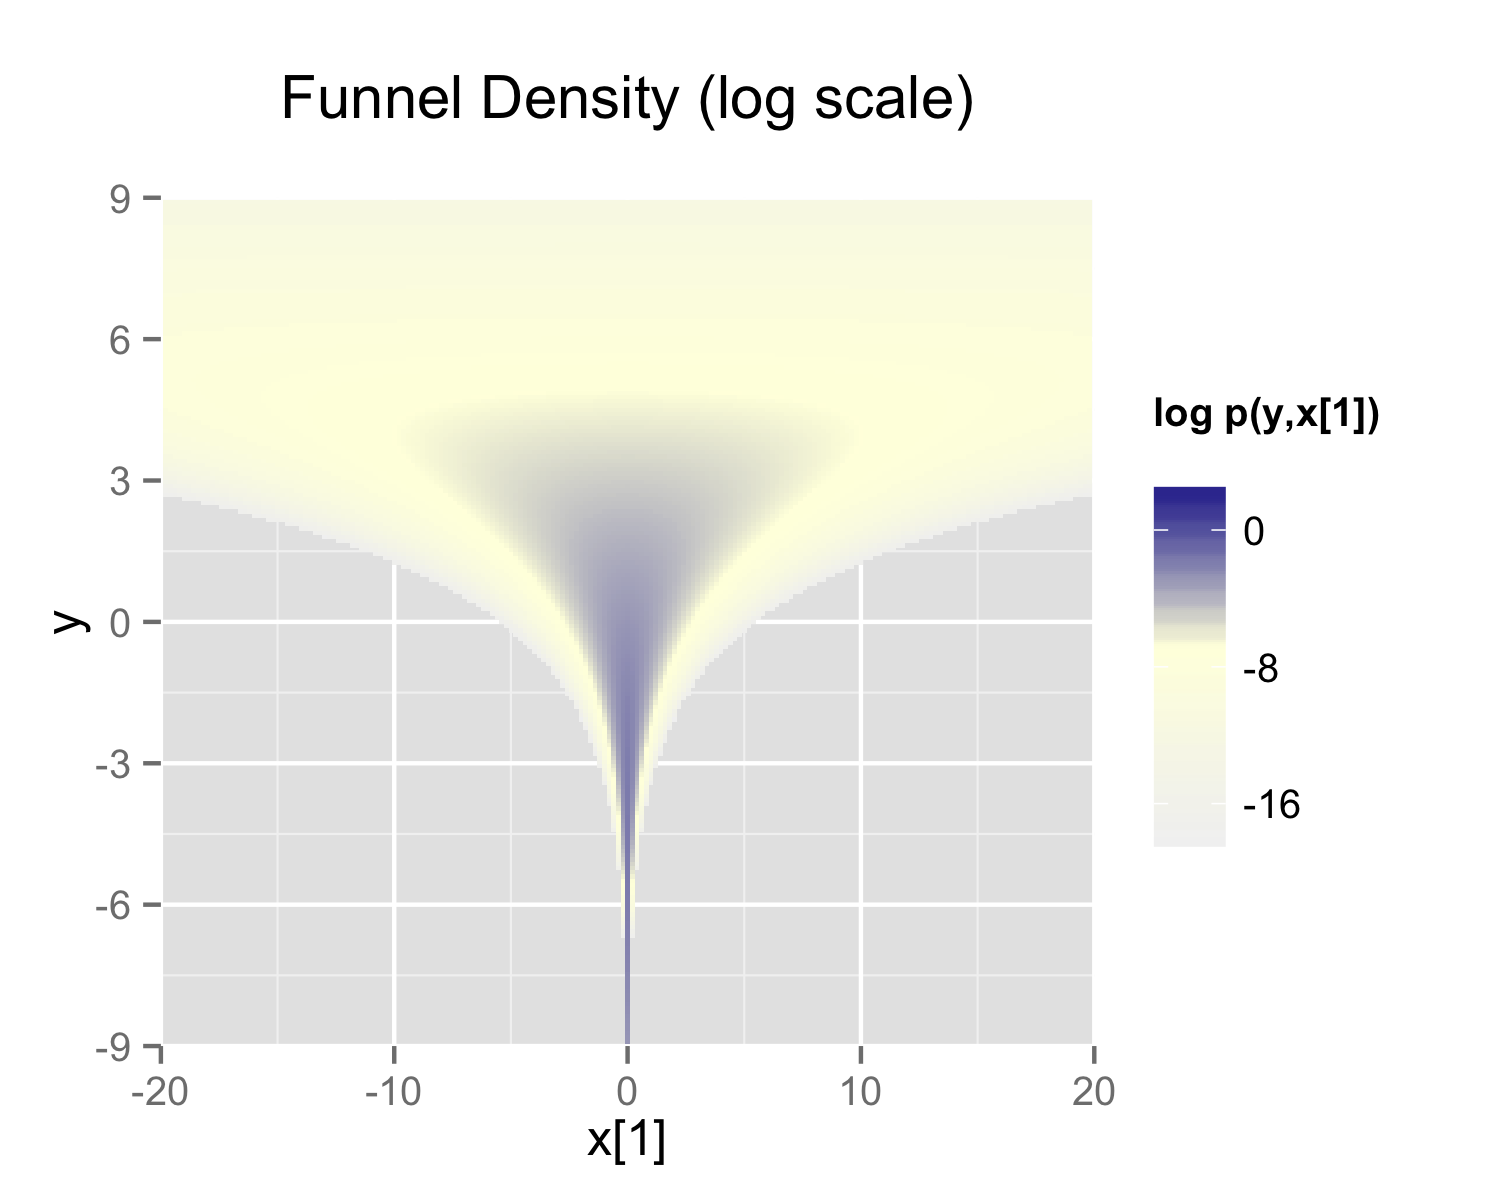
\includegraphics[height=2in]{img/funnel.png}
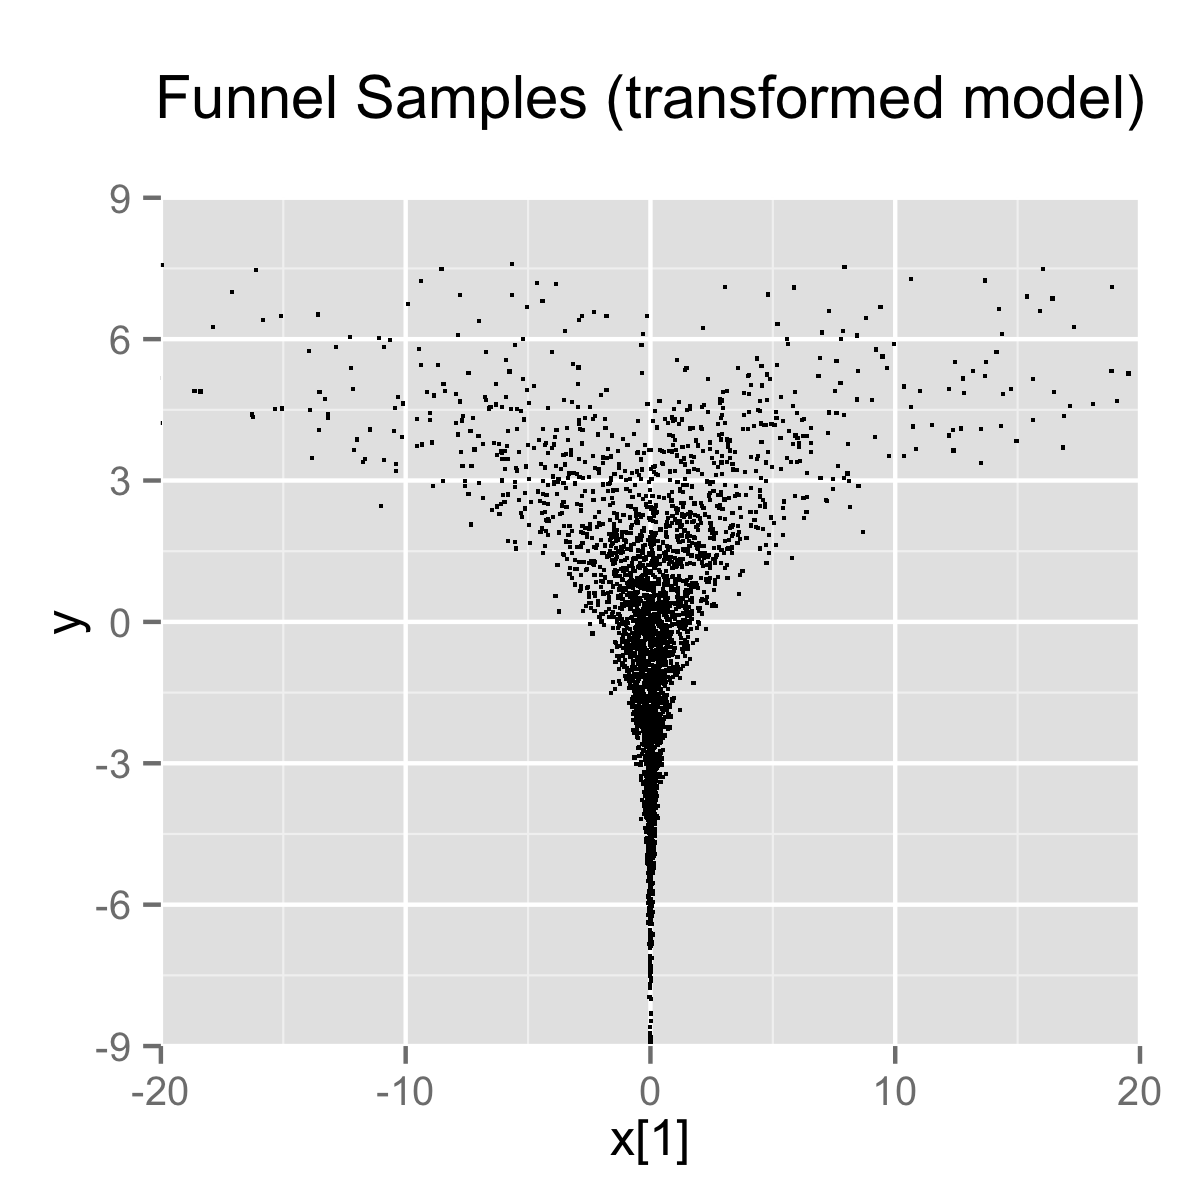
\includegraphics[height=2in]{img/funnel-fit.png}
\end{center}
\vspace*{-18pt}
\caption{\small\it Neal's Funnel.  (Left) The marginal density of
  Neal's funnel for the upper-level variable $y$ and one lower-level
  variable $x_1$ (see the text for the formula).  The blue region has
  log density greater than -8, the yellow region density greater than
  -16, and the gray background a density less than -16.  
  (Right) 4000 draws from a run of Stan's
  sampler with default settings.  Both plots are restricted to the
  shown window of $x_1$ and $y$ values; some draws fell outside of
  the displayed area as would be expected given the density.  The samples are
  consistent with the marginal density $p(y) =
  \distro{Normal}(y|0,3)$, which has mean 0 and standard deviation
  3.}\label{funnel.figure}
\end{figure}

\citep{Neal:2003} defines a distribution that exemplifies the
difficulties of sampling from some hierarchical models.  Neal's
example is fairly extreme, but can be trivially reparameterized in
such a way as to make sampling straightforward.

Neal's example has support for $y \in
\mathbb{R}$ and  $x \in \mathbb{R}^9$ with density
%
\[
p(y,x) = \distro{Normal}(y|0,3) \times \prod_{n=1}^9
\distro{Normal}(x_n|0,\exp(y/2)).
\]
%
The probability contours are shaped like ten-dimensional funnels.  The
funnel's neck is particularly sharp because of the exponential
function applied to $y$.  A plot of the log marginal density of $y$
and the first dimension $x_1$ is shown in \reffigure{funnel}.

The funnel can be implemented directly in Stan as follows.
%
\begin{quote}
\begin{Verbatim}[fontsize=\small]
parameters {  
  real y;
  vector[9] x;
}
model {
  y ~ normal(0,3);
  x ~ normal(0,exp(y/2));
}
\end{Verbatim}
\end{quote}
%
When the model is expressed this way, Stan has trouble sampling from
the neck of the funnel, where $y$ is small and thus $x$ is constrained
to be near 0.  This is due to the fact that the density's scale
changes with $y$, so that a step size that works well in the body will
be too large for the neck and a step size that works in the neck will be
very inefficient in the body.

In this particular instance, because the analytic form of the density
from which samples are drawn is known, the model can be converted to
the following more efficient form.
%
\begin{quote}
\begin{Verbatim}[fontsize=\small]
parameters {  
  real y_raw;
  vector[9] x_raw;
}
transformed parameters {
  real y;
  vector[9] x;

  y <- 3.0 * y_raw;  
  x <- exp(y/2) * x_raw;
}
model {
  y_raw ~ normal(0,1); // implies y ~ normal(0,3) 
  x_raw ~ normal(0,1); // implies x ~ normal(0,exp(y/2))  
}
\end{Verbatim}
\end{quote}
%
In this second model, the parameters \Verb|x_raw| and \Verb|y_raw| are
sampled as independent unit normals, which is easy for Stan.  These
are then transformed into samples from the funnel.  In this case, the
same transform may be used to define Monte Carlo samples directly
based on independent unit normal samples; Markov chain Monte Carlo
methods are not necessary. If such a reparameterization were used in
Stan code, it is useful to provide a comment indicating what the
distribution for the parameter implies for the distribution of the
transformed parameter.

\subsection{Reparameterizing the Cauchy}

Sampling from heavy tailed distributions such as the Cauchy is
difficult for Hamiltonian Monte Carlo, which operates within a
Euclidean geometry.%
\footnote{Riemannian Manifold Hamiltonian Monte Carlo (RMHMC) overcomes
  this difficulty by simulating the Hamiltonian dynamics in a a space
  with a position-dependent metric; see
  \citep{GirolamiCalderhead:2011} and \citep{Betancourt:2012}.}
%
The practical problem is that tail of the Cauchy
requires a relatively large step size compared to the trunk.  With a
small step size, the No-U-Turn sampler requires many steps when
starting in the tail of the distribution; with a large step size,
there will be too much rejection in the central portion of the
distribution.  This problem may be mitigated by defining the
Cauchy-distributed variable as the transform of a uniformly
distributed variable using the Cauchy inverse cumulative distribution
function.

Suppose a random variable of interest $X$ has a Cauchy distribution
with location $\mu$ and scale $\tau$, so that $X \sim
\distro{Cauchy}(\mu,\tau)$.  The variable $X$ has a cumulative
distribution function $F_X:\reals \rightarrow (0,1)$ defined by
\[
F_X(x) = \frac{1}{\pi} \arctan \left( \frac{x - \mu}{\tau} \right) +
\frac{1}{2}.
\]
The inverse of the cumulative distribution function,
$F_X^{-1}:(0,1) \rightarrow \reals$, is thus
%
\[
F^{-1}_X(y) = \mu + \tau \tan \left( \pi \left( x - \frac{1}{2} \right) \right).
\]
Thus if the random variable $Y$ has a unit uniform distribution, $Y
\sim \distro{Uniform}(0,1)$, then $F^{-1}_X(Y)$ has a Cauchy
distribution with location $\mu$ and scale $\tau$, i.e., $F^{-1}_X(Y) \sim
\distro{Cauchy}(\mu,\tau)$. 

Consider a Stan program involving a Cauchy-distributed parameter
\code{beta}.
%
\begin{quote}
\begin{Verbatim}[fontsize=\small]
parameters {
  real beta;
  ...
}
model {
  beta ~ cauchy(mu,tau);
  ...
}
\end{Verbatim}
\end{quote}
%
This declaration of \code{beta} as a parameter may be replaced with a
transformed parameter \code{beta} defined in terms of a
uniform-distributed parameter \code{beta\_unif}.
%
\begin{quote}
\begin{Verbatim}[fontsize=\small]
parameters {
  real<lower=-pi()/2, upper=pi()/2> beta_unif;
  ...
}
transformed parameters {
  real beta;
  beta <- mu + tau * tan(beta_unif);  // beta ~ cauchy(mu,tau)
}    
model {
  beta_unif ~ uniform(-pi()/2, pi()/2);  // not necessary
  ...
}
\end{Verbatim}
\end{quote}
%
It is more convenient in Stan to transform a uniform variable on
$(-\pi/2, \pi/2)$ than one on $(0,1)$.  The Cauchy location and scale
parameters, \code{mu} and \code{tau}, may be defined as data or may
themselves be parameters.  The variable \code{beta} could also be
defined as a local variable if it does not need to be included in the
sampler's output.

The uniform distribution on \code{beta\_unif} is defined explicitly in
the model block, but it could be safely removed from the program
without changing sampling behavior.  This is because $\log
\distro{Uniform}(\beta_{\mbox{\footnotesize unif}}|-\pi/2,\pi/2) =
-\log \pi$ is a constant and Stan only
needs the total log probability up to an additive constant.  Stan will spend
some time checking that that \code{beta\_unif} is between
\code{-pi()/2} and \code{pi()/2}, but this condition is guaranteed by
the constraints in the declaration of \code{beta\_unif}.  

\subsection{Reparameterizing a Student-t Distribution}

One thing that sometimes works when you're having trouble with the
heavy-tailedness of Student-t distributions is to use the
gamma-mixture representation, which says that you can generate a
Student-t distributed variable $\beta$,
\[
\beta \sim \mbox{\sf Student-t}(\nu, 0, 1),
\]
by first generating a gamma-distributed precision (inverse variance)
$\tau$ according to
\[
\tau \sim \mbox{\sf Gamma}(\nu/2, \nu/2),
\]
and then generating $\beta$ from the normal distribution,
\[
\beta \sim \mbox{\sf Normal}(0,\tau^{-\frac{1}{2}}).
\]
%
Because $\tau$ is precision, $\tau^{-\frac{1}{2}}$ is the scale
(standard deviation), which is the parameterization used by Stan.

The marginal distribution of $\beta$ when you integrate out $\tau$ is
$\mbox{\sf Student-t}(\nu, 0, 1)$, i.e.,
\[
\mbox{\sf Student-t}(\beta | \nu,0,1).
= 
\int_0^{\infty} 
\,
\mbox{\sf Normal}(\beta | 0, 1 / \tau^{-\frac{1}{2}})
\times
\mbox{\sf Gamma}(\tau | \nu/2, \nu/2)
\
d\tau.
\]
%

To go one step further, instead of defining a $\beta$ drawn from a
normal with precision $\tau$, define $\alpha$ to be drawn from a unit
normal,
%
\[
\alpha \sim \mbox{\sf Normal}(0,1)
\]
%
and rescale by defining
%
\[
\beta = \alpha \, \tau^{-\frac{1}{2}}.
\]
%

Now suppose $\mu = \beta x$ is the product of $\beta$ with a
regression predictor $x$.  Then the reparameterization $\mu = \alpha
\tau^{-\frac{1}{2}} x$ has the same distribution, but in the original, direct
parameterization, $\beta$ has (potentially) heavy tails, whereas in
the second, neither $\tau$ nor $\alpha$ have heavy tails.

To translate into Stan notation, this reparameterization replaces
%
\begin{quote}
\begin{Verbatim}
parameters {
  real<lower=0> nu;
  real beta;
  ...
model {
  beta ~ student_t(nu,0,1);
  ...
\end{Verbatim}
\end{quote}
%
with
%
\begin{quote}
\begin{Verbatim}
parameters {
  real<lower=0> nu;
  real<lower=0> tau;
  ...
transformed parameters {
  real beta;
  beta <- alpha / sqrt(tau);
  ...
model {
  real half_nu;
  half_nu <- 0.5 * nu;
  tau ~ gamma(half_nu, half_nu);
  alpha ~ normal(0, 1);
  ...
\end{Verbatim}
\end{quote}  
%
Although set to \code{0} here, in most cases, the lower bound for the
degrees of freedom parameter \code{nu} can be set to \code{1} or
higher; when \code{nu} is 1, the result is a Cauchy distribution with
very fat tails and as \code{nu} approaches infinity, the Student-t
distribution approaches a normal distribution.  Thus the parameter
\code{nu} characterizes the heaviness of the tails of the model.

\subsection{Hierarchical Models}

Unfortunately, the usual situation in applied Bayesian modeling
involves complex geometries and interactions that are not known
analytically.  Nevertheless, reparameterization can still be very
effective for separating parameters.  For example, a vectorized
hierarchical model might draw a vector of coefficients $\beta$ with
definitions as follows.
%
\begin{quote}
\begin{Verbatim}[fontsize=\small]
parameters {
  real mu_beta;   
  real<lower=0> sigma_beta;
  vector[K] beta;
  ...
model {
  beta ~ normal(mu_beta,sigma_beta);
  ...
\end{Verbatim}
\end{quote}
%
Although not shown, a full model will have priors on both
\Verb|mu_beta| and \Verb|sigma_beta| along with data modeled based on
these coefficients.  For instance, a standard binary logistic
regression with data matrix \code{x} and binary outcome vector
\code{y} would include a likelihood statement such as form
\Verb|y ~ bernoulli_logit(x * beta)|, leading to an analytically
intractable posterior.

A hierarchical model such as the above will suffer from the same kind
of inefficiencies as Neal's funnel, though typically not so extreme,
because the values of \Verb|beta|, \Verb|mu_beta| and
\Verb|sigma_beta| are highly correlated in the posterior. When there is a lot of data, such a
hierarchical model can be made much more efficient by shifting the data's correlation with the 
parameters to the hyperparameters. Similar to the funnel example, this will be much more 
efficient in terms of effective sample size~\citep{Betancourt-Girolami:2013}.
%
\begin{quote}
\begin{Verbatim}[fontsize=\small]
parameters {
  vector[K] beta_raw;
  ...
transformed parameters {
  vector[K] beta;
  // implies: beta ~ normal(mu_beta,sigma_beta)
  beta <- mu_beta + sigma_beta * beta_raw;
model {
  beta_raw ~ normal(0,1);  
  ...
\end{Verbatim}
\end{quote}
%
Any priors defined for \Verb|mu_beta| and \Verb|sigma_beta| remain as
defined in the original model.

Reparameterization of hierarchical models is not limited to the normal
distribution, although the normal distribution is the best candidate
for doing so. In general, any distribution of parameters in the 
location-scale family is a good candidate for reparameterization. Let
$\beta = l + s\alpha$ where $l$ is a location parameter and $s$ is a
scale parameter. Note that $l$ need not be the mean, $s$ need not
be the standard deviation, and neither the mean nor the standard
deviation need to exist. If $\alpha$ and $\beta$ are from the same
distributional family but $\alpha$ has location zero and unit scale, 
while $\beta$ has location $l$ and scale $s$, then that distribution
is a location-scale distribution. Thus, if $\alpha$ were a parameter
and $\beta$ were a transformed parameter, then a prior distribution
from the location-scale family on $\alpha$ with location zero and unit 
scale implies a prior distribution on $\beta$ with location $l$ and
scale $s$. Doing so would reduce the dependence between $\alpha$, 
$l$, and $s$.

There are several univariate distributions in the location-scale
family, such as the Student t distribution, including its special
cases of the Cauchy distribution (with one degree of freedom) and the
normal distribution (with infinite degrees of freedom). As shown above,
if $\alpha$ is distributed standard normal, then $\beta$ is distributed
normal with mean $\mu = l$ and standard deviation $\sigma = s$. The 
logistic, the double exponential, the generalized extreme value 
distributions, and the stable distribution are also in the 
location-scale family.

Also, if $z$ is distributed standard normal, then $z^2$ is distributed
chi-squared with one degree of freedom. By summing the squares of $K$
independent standard normal variates, one can obtain a single variate
that is distributed chi-squared with $K$ degrees of freedom. However,
for large $K$, the computational gains of this reparameterization may
be overwhelmed by the computational cost of specifying $K$ primitive
parameters just to obtain one transformed parameter to use in a model.

\subsection{Multivariate Reparameterizations}

The benefits of reparameterization are not limited to univariate 
distributions. A parameter with a multivariate normal prior distribution
is also an excellent candidate for reparameterization. Suppose you intend
the prior for $\beta$ to be multivariate normal with mean vector $\mu$
and covariance matrix $\Sigma$. Such a belief is reflected by the
following code.
%
\begin{quote}
\begin{Verbatim}[fontsize=\small]
data {
  int<lower=2> K;
  vector[K] mu;
  cov_matrix[K] Sigma;
  ...
parameters {
  vector[K] beta;
  ...
model {
  beta ~ multi_normal(mu,Sigma);
  ...
\end{Verbatim}
\end{quote}
%
In this case \Verb|mu| and \Verb|Sigma| are fixed data, but they could
be unknown parameters, in which case their priors would be unaffected
by a reparameterization of \Verb|beta|.

If $\alpha$ has the same dimensions as $\beta$ but the elements of 
$\alpha$ are independently and identically distributed standard normal 
such that $\beta = \mu + L\alpha$, where $LL^\top = \Sigma$, then 
$\beta$ is distributed multivariate normal with mean vector $\mu$ and 
covariance matrix $\Sigma$. One choice for $L$ is the Cholesky factor
of $\Sigma$. Thus, the model above could be reparameterized as follows.
%
\begin{quote}
\begin{Verbatim}[fontsize=\small]
data {
  int<lower=2> K;
  vector[K] mu;
  cov_matrix[K] Sigma;
  ...
transformed data {
  matrix[K,K] L;
  L <- cholesky_decompose(Sigma);
}
parameters {
  vector[K] alpha;
  ...
transformed parameters {
  vector[K] beta;
  beta <- mu + L * alpha; 
}
model {
  alpha ~ normal(0,1); 
  // implies: beta ~ multi_normal(mu, Sigma)
  ...
\end{Verbatim}
\end{quote}
%
This reparameterization is more efficient for two reasons. First, it
reduces dependence among the elements of \Verb|alpha| and second, it
avoids the need to invert \Verb|Sigma| every time \Verb|multi_normal|
is evaluated.

The Cholesky factor is also useful when a covariance matrix is 
decomposed into a correlation matrix that is multiplied from both
sides by a diagonal matrix of standard deviations, where either the
standard deviations or the correlations are unknown parameters. The
Cholesky factor of the covariance matrix is equal to the product of
a diagonal matrix of standard deviations and the Cholesky factor of
the correlation matrix. Furthermore, the product of a diagonal matrix
of standard deviations and a vector is equal to the elementwise
product between the standard deviations and that vector. Thus, if for
example the correlation matrix \Verb|Tau| were fixed data but the
vector of standard deviations \Verb|sigma| were unknown parameters,
then a reparameterization of \Verb|beta| in terms of \Verb|alpha|
could be implemented as follows.
%
\begin{quote}
\begin{Verbatim}[fontsize=\small]
data {
  int<lower=2> K;
  vector[K] mu;
  corr_matrix[K] Tau;
  ...
transformed data {
  matrix[K,K] L;
  L <- cholesky_decompose(Tau);
}
parameters {
  vector[K] alpha;
  vector<lower=0>[K] sigma;
  ...
transformed parameters {
  vector[K] beta;
  // This equals mu + diag_matrix(sigma) * L * alpha;
  beta <- mu + sigma .* (L * alpha);
}
model {
  sigma ~ cauchy(0,5);
  alpha ~ normal(0,1);
  // implies: beta ~ multi_normal(mu,
  //  diag_matrix(sigma) * L * L' * diag_matrix(sigma)))
  ...
\end{Verbatim}
\end{quote}
%
This reparameterization of a multivariate normal distribution in
terms of standard normal variates can be extended to other multivariate
distributions that can be conceptualized as contaminations of the 
multivariate normal, such as the multivariate Student t and the skew
multivariate normal distribution.

A Wishart distribution can also be reparameterized in terms of standard
normal variates and chi-squared variates. Let $L$ be the Cholesky factor
of a $K \times K$ positive definite scale matrix $S$ and let $\nu$ be
the degrees of freedom. If
%
\begin{equation*}
A = \left( \begin{array}{cccc}
\sqrt{c_{1}} & 0 & \cdots & 0\\
z_{21} & \sqrt{c_{2}} & \ddots & \vdots\\
\vdots & \ddots & \ddots & 0\\
z_{K1} & \cdots & z_{K\left(K-1\right)} & \sqrt{c_{K}}
 \end{array} \right),
\end{equation*}
%
where each $c_i$ is distributed chi-squared with $\nu - i + 1$ degrees
of freedom and each $z_{ij}$ is distributed standard normal, then
$W = LAA^{\top}L^{\top}$ is distributed Wishart with scale matrix
$S = LL^{\top}$ and degrees of freedom $\nu$. Such a reparameterization
can be implemented by the following Stan code:
%
\begin{quote}
\begin{Verbatim}[fontsize=\small]
data {
  int<lower=1> N;
  int<lower=1> K;
  int<lower=K+2> nu
  matrix[K,K] L; // Cholesky factor of scale matrix
  vector[K] mu;
  matrix[N,K] y;
  ...
parameters {
  vector<lower=0>[K] c;
  vector[0.5 * K * (K - 1)] z;
  ...
model {
  matrix[K,K] A;
  int count;
  count <- 1;
  for (j in 1:(K-1)) {
    for (i in (j+1):K) {
      A[i,j] <- z[count];
      count <- count + 1;
    }
    for (i in 1:(j - 1)) {
      A[i,j] <- 0.0;
    }
    A[j,j] <- sqrt(c[j]);
  }
  
  for (i in 1:K) {
    c[i] ~ chi_square(nu - i + 1);
  }
  z ~ normal(0,1);
  // implies: L * A * A' * L' ~ wishart(nu, L * L')
  y ~ multi_normal_cholesky(mu, L * A);
  ...
\end{Verbatim}
\end{quote}
%
This reparameterization is more efficient for three reasons. First, it
reduces dependence among the elements of \Verb|z| and second, it
avoids the need to invert the covariance matrix, $W$ every time 
\Verb|wishart| is evaluated. Third, if $W$ is to be used with a
multivariate normal distribution, you can pass $L A$ to the more
efficient \Verb|multi_normal_cholesky| function, rather than passing
$W$ to \Verb|multi_normal|.

If $W$ is distributed Wishart with scale matrix $S$ and degrees of
freedom $\nu$, then $W^{-1}$ is distributed inverse Wishart with inverse
scale matrix $S^{-1}$ and degrees of freedom $\nu$. Thus, the previous
result can be used to reparameterize the inverse Wishart distribution.
Since $W = L * A * A^{\top} * L^{\top}$, 
$W^{-1} = L^{{\top}^{-1}} A^{{\top}^{-1}} A^{-1} L^{-1}$, where all four
inverses exist, but 
$L^{{-1}^{\top}} = L^{{\top}^{-1}}$ and $A^{{-1}^{\top}} = A^{{\top}^{-1}}$.
We can slightly modify the above Stan code for this case:
%
\begin{quote}
\begin{Verbatim}[fontsize=\small]
data {
  int<lower=1> K;
  int<lower=K+2> nu
  matrix[K,K] L; // Cholesky factor of scale matrix
  ...
transformed data {
  matrix[K,K] eye;
  matrix[K,K] L_inv;
  for (j in 1:K) {
    for (i in 1:K) {
      eye[i,j] <- 0.0;
    }
    eye[j,j] <- 1.0;
  }
  L_inv <- mdivide_left_tri_low(L, eye);
}
parameters {
  vector<lower=0>[K] c;
  vector[0.5 * K * (K - 1)] z;
  ...
model {
  matrix[K,K] A;
  matrix[K,K] A_inv_L_inv;  
  int count;
  count <- 1;
  for (j in 1:(K-1)) {
    for (i in (j+1):K) {
      A[i,j] <- z[count];
      count <- count + 1;
    }
    for (i in 1:(j - 1)) {
      A[i,j] <- 0.0;
    }
    A[j,j] <- sqrt(c[j]);
  }
  A_inv_L_inv <- mdivide_left_tri_low(A, L_inv);
  for (i in 1:K) {
    c[i] ~ chi_square(nu - i + 1);
  }
  z ~ normal(0,1); // implies: crossprod(A_inv_L_inv) ~ 
  // inv_wishart(nu, L_inv' * L_inv)
  ...
\end{Verbatim}
\end{quote}
%
Another candidate for reparameterization is the Dirichlet distribution
with all $K$ shape parameters equal. \cite{ZyczkowskiSommers:2001} shows 
that if $\theta_i$ is equal to the sum of $\beta$ independent squared 
standard normal variates and $\rho_i = \frac{\theta_i}{\sum \theta_i}$, 
then the $K$-vector $\rho$ is distributed Dirichlet with all shape 
parameters equal to $\frac{\beta}{2}$. In particular, if $\beta = 2$, 
then $\rho$ is uniformly distributed on the unit simplex. Thus, we can 
make $\rho$ be a transformed parameter to reduce dependence, as in:
%
\begin{quote}
\begin{Verbatim}[fontsize=\small]
data {
  int<lower=1> beta;
  ...
parameters {
  vector[beta] z[K];
  ...
transformed parameters {
  simplex[K] rho;
  for (k in 1:K)
    rho[k] <- dot_self(z[k]); // sum-of-squares
  rho <- rho / sum(rho);
}
model {
  for (k in 1:K)
    z[k] ~ normal(0,1); 
  // implies: rho ~ dirichlet(0.5 * beta * ones)
  ...
\end{Verbatim}
\end{quote}
%

\section{Vectorization}

\subsection{Gradient Bottleneck}

\Stan spends the vast majority of its time computing the gradient of
the log probability function, making gradients the obvious target for
optimization.  \Stan's gradient calculations with algorithmic
differentiation require a template expression to be allocated%
%
\footnote{\Stan uses its own arena-based allocation, so allocation and
  deallocation are faster than with a raw call to \code{new}.}
%
and constructed for each subexpression of a \Stan program involving
parameters or transformed parameters.  This section defines
optimization strategies based on vectorizing these subexpressions to
reduce the work done during algorithmic differentiation.

\subsection{Vectorizing Summations}

Because of the gradient bottleneck described in the previous section,
it is more efficient to collect a sequence of summands into a vector
or array and then apply the \code{sum()} operation than it is to
continually increment a variable by assignment and addition.  For
example, consider the following code snippet, where \code{foo()} is
some operation that depends on \code{n}.
%
\begin{quote}
\begin{Verbatim}[fontsize=\small]
for (n in 1:N) 
  total <- total + foo(n,...);
\end{Verbatim}
\end{quote}
%
This code has to create intermediate representations for each
of the \code{N} summands.  

A faster alternative is to copy the values into a vector, then
apply the \code{sum()} operator, as in the following refactoring.
%
\begin{quote}
\begin{Verbatim}[fontsize=\small]
{  
  vector[N] summands;
  for (n in 1:N) 
    summands[n] <- foo(n,...);
  total <- sum(summands);
}
\end{Verbatim}
\end{quote}
%
Syntactically, the replacement is a statement block delineated
by curly brackets (\Verb|{|, \Verb|}|), starting with the definition
of the local variable \code{summands}.

Even though it involves extra work to allocate the \code{summands}
vector and copy \code{N} values into it, the savings in
differentiation more than make up for it.  Perhaps surprisingly,
it will also use substantially less memory overall than incrementing
\code{total} within the loop.


\subsection{Vectorization through Matrix Operations}

The following program directly encodes a linear regression with fixed
unit noise using a two-dimensional array \code{x} of predictors, an
array \code{y} of outcomes, and an array \code{beta} of regression
coefficients.
%
\begin{quote}
\begin{Verbatim}[fontsize=\small]
data {
  int<lower=1> K;
  int<lower=1> N;
  real x[K,N];
  real y[N];
}
parameters {
  real beta[K];
}
model {
  for (n in 1:N) {
    real gamma;  
    gamma <- 0.0;
    for (k in 1:K)
      gamma <- gamma + x[n,k] * beta[k];
    y[n] ~ normal(gamma,1);
  }
}
\end{Verbatim}
\end{quote}
%
The following model computes the same log probability function as the
previous model, even supporting the same input files for data and
initialization.
%
\begin{quote}
\begin{Verbatim}[fontsize=\small]
data {
  int<lower=1> K;
  int<lower=1> N;
  vector[K] x[N];
  real y[N];
}
parameters {
  vector[K] beta;
}
model {
  for (n in 1:N)
    y[n] ~ normal(dot_product(x[n],beta), 1);
}
\end{Verbatim}
\end{quote}
%
Although it produces equivalent results, the dot product should not be
replaced with a transpose and multiply, as in
%
\begin{quote}
\begin{Verbatim}[fontsize=\small]
        y[n] ~ normal(x[n]' * beta, 1);
\end{Verbatim}
\end{quote}
%
The relative inefficiency of the transpose and multiply approach is
that the transposition operator allocates a new vector into which the
result of the transposition is copied.  This consumes both time
and memory\footnote{Future versions of \Stan may remove this inefficiency
by more fully exploiting expression templates inside the Eigen
\Cpp matrix library.  This will require enhancing Eigen to deal
with mixed-type arguments, such as the type \code{double} used
for constants and the algorithmic differentiation type
\code{stan::agrad::var} 
used for variables.}.
%
The inefficiency of transposition could itself be mitigated somewhat by
reordering the product and pulling the transposition out of the loop,
as follows.
%
\begin{quote}
\begin{Verbatim}[fontsize=\small]
...
transformed parameters {
  row_vector[K] beta_t;
  beta_t <- beta';
}
model {
  for (n in 1:N)
    y[n] ~ normal(beta_t * x[n], 1);
}
\end{Verbatim}
\end{quote}
%
The problem with transposition could be completely solved by directly
encoding the \code{x} as a row vector, as in the
following example.
%
\begin{quote}
\begin{Verbatim}[fontsize=\small]
data {
  ...
  row_vector[K] x[N];
  ...
}
parameters {
  vector[K] beta;
}
model {
  for (n in 1:N)
    y[n] ~ normal(x[n] * beta, 1);
}
\end{Verbatim}
\end{quote}
%
Declaring the data as a matrix and then computing all the predictors
at once using matrix multiplication is more efficient still, as in the
example discussed in the next section.

\subsection{Vectorized Probability Functions}

The final and most efficient version replaces the loops and
transformed parameters by using the vectorized form of the normal
probability function, as in the following example.
%
\begin{quote}
\begin{Verbatim}[fontsize=\small]
data {
  int<lower=1> K;
  int<lower=1> N;
  matrix[N,K] x;
  vector[N] y;
}
parameters {
  vector[K] beta;
} 
model {
  y ~ normal(x * beta, 1);
}
\end{Verbatim}
\end{quote}
%
The variables are all declared as either matrix or vector types.
The result of the matrix-vector multiplication \code{x * beta} in the
model block is a vector of the same length as \code{y}.  

The probability function documentation in \refpart{built-in-functions}
indicates which of \Stan's probability functions support
vectorization; see \refsection{prob-vectorization} for more
information.  Vectorized probability functions accept either vector or
scalar inputs for all arguments, with the only restriction being that
all vector arguments are the same dimensionality.  In the example
above, \code{y} is a vector of size \code{N}, \code{x * beta} is a
vector of size \code{N}, and \code{1} is a scalar.

\section{Exploiting Sufficient Statistics}

In some cases, models can be recoded to exploit sufficient statistics
in estimation.  This can lead to large efficiency gains compared to an
expanded model.  For example, consider the following Bernoulli
sampling model.
%
\begin{quote}
\begin{Verbatim}[fontsize=\small]
data {
  int<lower=0> N;
  int<lower=0,upper=1> y[N];
  real<lower=0> alpha;
  real<lower=0> beta;
}
parameters {
  real<lower=0,upper=1> theta;
}
model {
  theta ~ beta(alpha,beta);
  for (n in 1:N) 
    y[n] ~ bernoulli(theta);
}
\end{Verbatim}
\end{quote}
%
In this model, the sum of positive outcomes in \code{y} is a
sufficient statistic for the chance of success \code{theta}.  The
model may be recoded using the binomial distribution as follows.
%
\begin{quote}
\begin{Verbatim}[fontsize=\small]
    theta ~ beta(alpha,beta);
    sum(y) ~ binomial(N,theta);
\end{Verbatim}
\end{quote}
%
Because truth is represented as one and falsehood as zero, the sum
\code{sum(y)} of a binary vector \code{y} is equal to the number of
positive outcomes out of a total of \code{N} trials.  



\section{Exploiting Conjugacy}


Continuing the model from the previous section, the conjugacy of the
beta prior and binomial sampling distribution allow the model to be
further optimized to the following equivalent form.
%
\begin{quote}
\begin{Verbatim}[fontsize=\small]
    theta ~ beta(alpha + sum(y), beta + N - sum(y));
\end{Verbatim}
\end{quote}
%
To make the model even more efficient, a transformed data variable
defined to be \code{sum(y)} could be used in the place of \code{sum(y)}.

\section{Standardizing Predictors and Outputs}

Stan programs will run faster if the input is standardized to have a
zero sample mean and unit sample variance.  This section illustrates
the principle with a simple linear regression.

Suppose that $y = (y_1,\ldots,y_N)$ is a sequence of $N$ outcomes and
$x = (x_1,\ldots,x_N)$ a parallel sequence of $N$ predictors.  A
simple linear regression involving an intercept coefficient $\alpha$
and slope coefficient $\beta$ can be expressed as
\[
y_n = \alpha + \beta x_n + \epsilon_n,
\]
where
\[
\epsilon_n \sim \distro{Normal}(0,\sigma).
\]

If either vector $x$ or $y$ has very large or very small values or if the
sample mean of the values is far away from 0 (on the scale of the values),
then it can be more efficient to standardize the outputs $y_n$ and
predictors $x_n$.  The data is first centered by subtracting the
sample mean, and then scaled by dividing by the sample deviation.
Thus a data point $u$ is standardized is standardized with respect to
a vector $y$  by the function $\mbox{z}_y$, defined by
\[
\mbox{z}_y(u) = \frac{u - \bar{y}}{\mbox{sd}(y)}
\]
where the sample mean of $y$ is
\[
\bar{y}
= \frac{1}{N} \sum_{n=1}^N y_n,
\]
and the sample standard deviation of $y$ is
\[
\mbox{sd}(y) 
= \left( 
\frac{1}{N} \sum_{n=1}^N (y_n - \bar{y})^2
\right)^{1/2}.
\]
The inverse transform is
defined by reversing the two normalization steps, first rescaling by
the same deviation and relocating by the sample mean,
\[
\mbox{z}^{-1}(v) = \mbox{sd}(y) v + \bar{y}.
\]

To standardize a regression problem, the predictors and outcomes are
standardized.  This changes the scale of the variables, and hence
changes the scale of the priors.  Consider the following initial
model.
%
\begin{quote}
\begin{Verbatim}[fontsize=\small]
data {
  int<lower=0> N;
  vector[N] y;
  vector[N] x;
}
parameters {
  real alpha;
  real beta;
  real<lower=0> sigma;
}
model {
  // priors
  alpha ~ normal(0,10);    
  beta ~ normal(0,10);
  sigma ~ cauchy(0,5);
  // likelihood
  for (n in 1:N)
    y[n] ~ normal(alpha + beta * x[n], sigma);
}
\end{Verbatim}
\end{quote}
%

The data block for the standardized model is identical.  The
standardized predictors and outputs are defined in the transformed
data block.  
%
\begin{quote}
\begin{Verbatim}[fontsize=\small]
data {
  int<lower=0> N;
  vector[N] y;
  vector[N] x;
}
transformed data {
  vector[N] x_std;
  vector[N] y_std;
  x_std <- (x - mean(x)) / sd(x);
  y_std <- (y - mean(y)) / sd(y);
}
parameters {
  real alpha_std;
  real beta_std;
  real<lower=0> sigma_std;
}
model {
  alpha_std ~ normal(0,10);    
  beta_std ~ normal(0,10);
  sigma_std ~ cauchy(0,5);
  for (n in 1:N)
    y_std[n] ~ normal(alpha_std + beta_std * x_std[n], 
                      sigma_std);
}
\end{Verbatim}
\end{quote}
%
The parameters are renamed to indicate that they aren't the
``natural'' parameters, but the model is otherwise identical.  In
particular, the fairly diffuse priors on the coefficients and error
scale are the same.  These could have been transformed as well, but
here they are left as is, because the scales make sense as very
diffuse priors for standardized data; the priors could be made more
informative.  For instance, because the outputs $y$ have been
standardized, the error $\sigma$ should not be greater than 1, because
that's the scale of the noise for predictors $\alpha = \beta = 0$.

The original regression
\[
y_n 
= \alpha + \beta x_n + \epsilon_n
\]
has been transformed to a regression on the standardized variables,
\[
\mbox{z}_y(y_n)
= \alpha'
+ \beta' \mbox{z}_x(x_n)
+ \epsilon'_n.
\]
The original parameters can be recovered with a little algebra,
%
\begin{eqnarray*}
y_n 
& = & \mbox{z}_y^{-1}(\mbox{z}_y(y_n))
\\[4pt]
& = & 
\mbox{z}_y^{-1} 
\left( 
\alpha' 
+ \beta' \mbox{z}_x(x_n)
+ \epsilon_n'
\right)
\\[4pt]
& = & 
\mbox{z}_y^{-1} 
\left( 
\alpha' 
+ \beta' 
    \left(  
      \frac{x_n - \bar{x}}{\mbox{\small sd}(x)}
    \right)
+ \epsilon_n'
\right)
\\[4pt]
& = & 
\mbox{sd}(y)
\left( 
\alpha' 
+ \beta' 
    \left(  
      \frac{x_n - \bar{x}}{\mbox{\small sd}(x)}
    \right)
+ \epsilon_n'
\right)
+ \bar{y}
\\[4pt]
& = & 
\left( 
  \mbox{sd}(y) 
      \left( 
          \alpha' 
          - \beta' \frac{\bar{x}}{\mbox{\small sd}(x)}
      \right) 
  + \bar{y}  
\right)
+ \left(
      \beta' \frac{\mbox{\small sd}(y)}{\mbox{\small sd}(x)} 
  \right) x_n
+ \mbox{sd}(y) \epsilon'_n,
\end{eqnarray*}
%
from which the original scale parameter values can be read off,
\[
\alpha 
=
\mbox{sd}(y) 
      \left( 
          \alpha' 
          - \beta' \frac{\bar{x}}{\mbox{\small sd}(x)}
      \right) 
  + \bar{y};
\ \ \ \ \ 
\beta = \beta' \frac{\mbox{\small sd}(y)}{\mbox{\small sd}(x)};
\ \ \ \ \
\sigma = \mbox{sd}(y) \sigma'.
\]
%
These recovered parameter values on the original scales can be
calculated within Stan using a generated quantities block following
the model block,
\begin{quote}
\begin{Verbatim}[fontsize=\small]
generated quantities {
  real alpha;
  real beta;
  real<lower=0> sigma;
  alpha <- sd(y) * (alpha_std - beta_std * mean(x) / sd(x)) 
           + mean(y);
  beta <- beta_std * sd(y) / sd(x);
  sigma <- sd(y) * sigma_std;
}
\end{Verbatim}
\end{quote}
%
Of course, it is inefficient to compute all of the means and standard
deviations every iteration; for more efficiency, these can be
calculated once and stored as transformed data.  Furthermore, the
model sampling statement can be easily vectorized, for instance, in
the transformed model, to
\begin{quote}
\begin{Verbatim}[fontsize=\small]
    y_std ~ normal(alpha_std + beta_std * x_std, sigma_std);
\end{Verbatim}
\end{quote}



\chapter{Reproducibility}\label{reproducibility.chapter}

\noindent
Floating point operations on modern computers are notoriously
difficult to replicate because the fundamental arithmetic operations,
right down to the IEEE 754 encoding level, are not fully specified.
The primary problem is that the precision of operations varies across
different hardware platforms and software implementations.

Stan is designed to allow full reproducibility.  However, this is only
possible up to the external constraints imposed by floating point
arithmetic.

Stan results will only be exactly reproducible if {\it all}\, of the following
components are {\it identical}\,:
%
\begin{itemize}
\item Stan version
\item Stan interface (RStan, PyStan, CmdStan) and version, plus version
  of interface language (R, Python, shell)
\item versions of included libraries (Boost and Eigen)
\item operating system version
\item computer hardware including CPU, motherboard and memory
\item \Cpp compiler, including version, compiler flags, and linked libraries
\item same configuration of call to Stan, including random seed, chain
  ID, initialization and data
\end{itemize}
%
It doesn't matter if you use a stable release version of Stan or the
version with a particular Git hash tag.  The same goes for all of the
interfaces, compilers, and so on on.  The point is that if any of
these moving parts changes in some way, floating point results may
change.

Concretely, if you compile a single Stan program using the same
CmdStan code base, but changed the optimization flag (\code{-O3} vs.\
\code{-O2} or \code{-O0}), the two programs may not return the identical
stream of results.  Thus it is very hard to guarantee reproducibility
on externally managed hardware, like in a cluster or even a desktop
managed by an IT department or with automatic updates turned on.

If, however, you compiled a Stan program today using one set of flags,
took the computer away from the internet and didn't allow it to update
anything, then came back in a decade and recompiled the Stan program
in the same way, you should get the same results.

The data needs to be the same down to the bit level. For example, if
you are running in RStan, Rcpp handles the conversion between R's
floating point numbers and C++ doubles. If Rcpp changes the conversion
process or use different types, the results are not guaranteed to be
the same down to the bit level.  
